%% LaTeX2e class for student theses
%% thesis.tex
%% 
%% Karlsruhe Institute of Technology
%% Institute for Program Structures and Data Organization
%% Chair for Software Design and Quality (SDQ)
%%
%% Dr.-Ing. Erik Burger
%% burger@kit.edu
%%
%% See https://sdq.kastel.kit.edu/wiki/Dokumentvorlagen
%%
%% Version 1.4, 2023-06-19

%% Available page modes: oneside, twoside
%% Available languages: english, ngerman
%% Available modes: draft, final (see README)
\documentclass[twoside, english, final]{sdqthesis}

%% Todonotes package
\usepackage[obeyFinal]{todonotes}
\setuptodonotes{inline}
\setuptodonotes{inlinewidth=0.95\linewidth}

%% Nowidow package
\usepackage[defaultlines=3,all]{nowidow}

%% Subcaption package required for subfigures
\usepackage{subcaption}

%% Glossaries package required for acronym section
\usepackage[acronym,toc,section=chapter,numberedsection=false,style=listgroup]{glossaries}
\makeglossaries
\loadglsentries{sections/acronyms.tex}

%% Cleveref package
\usepackage{cleveref}

\usepackage{amsmath}

\usepackage{algorithm}
\usepackage{algpseudocode}
\algrenewcommand\algorithmiccomment[1]{//~#1}
\newcommand*\LineComment[1]{\State //~#1}
\newcommand*\ForIn[2]{\ForAll{#1 $\in$ #2}}
\newcommand*\Let[2]{\State #1 $\gets$ #2}

%% ---------------------------------
%% | Information about the thesis  |
%% ---------------------------------

%% Name of the author
\author{Moritz Gstür}

%% Title (and possibly subtitle) of the thesis
\title{Certificateless Attribute-Based Server-Aided Cryptosystem for Substation Automation Systems (CASC-SAS)}

%% Type of the thesis 
\thesistype{Master's Thesis}

%% Change the institute here, ``KASTEL'' is default
\myinstitute{Institute for Automation and Applied Informatics (IAI)}

%% You can put a logo in the ``logos'' directory and include it here
%% instead of the SDQ logo
% \grouplogo{myfile}
%% Alternatively, you can disable the group logo
\nogrouplogo

%% The reviewers are the professors that grade your thesis
\reviewerone{Prof. Dr. Veit Hagenmeyer}
\reviewertwo{Prof. Dr. Achim Streit}

%% The advisors are PhDs or Postdocs
\advisorone{Dr. Mohammed Ramadan}
%% The second advisor can be omitted
\advisortwo{Dr.-Ing. Ghada Elbez}

%% Please enter the start end end time of your thesis
\editingtime{01. August 2024}{03. February 2025}

\settitle

%% --------------------------------
%% | Bibliography                 |
%% --------------------------------

%% Use biber instead of BibTeX, see README
\usepackage[citestyle=numeric,style=numeric,sorting=none,maxcitenames=2,backend=biber]{biblatex}
\addbibresource{../bibliography/masterthesis.bib}

%% ====================================
%% ====================================
%% ||                                ||
%% || Beginning of the main document ||
%% ||                                ||
%% ====================================
%% ====================================
\begin{document}

%% Set PDF metadata
\setpdf

%% Set the title
\maketitle

%% The Preamble begins here
\frontmatter

%% LaTeX2e class for student theses: Declaration of independent work
%% sections/declaration.tex
%% 
%% Karlsruhe Institute of Technology
%% Institute of Information Security and Dependability
%% Software Design and Quality (SDQ)
%%
%% Dr.-Ing. Erik Burger
%% burger@kit.edu
%%
%% Version 1.5, 2024-02-12

\thispagestyle{empty}
\null\vfill
\noindent\hbox to \textwidth{\hrulefill} 
%
% Gemäß Studien- und Prüfungsordnung Bachelor Informatik des KIT,
% § 14 (5) vom 10.05.2022
% 
\iflanguage{english}{I declare that I have developed and written the enclosed
thesis completely by myself. 
I have not used any other than the aids that I have mentioned. 
I have marked all parts of the thesis that I have included from 
referenced literature, either in their original wording or paraphrasing their
contents. 
I have followed the by-laws to implement scientific integrity at KIT.}%
{Ich versichere wahrheitsgemäß, die Arbeit selbstständig verfasst, alle benutzten 
Quellen und Hilfsmittel vollständig und genau angegeben und alles kenntlich gemacht 
zu haben, was aus Arbeiten anderer unverändert oder mit Abänderungen entnommen wurde 
sowie die Satzung des KIT zur Sicherung guter wissenschaftlicher Praxis in der 
jeweils gültigen Fassung beachtet zu haben. }
 
 
%% ---------------------------------------------
%% | Replace PLACE and DATE with actual values |
%% ---------------------------------------------
\textbf{Karlsruhe, 05. August 2024}
\vspace{1.5cm}
 
\dotfill\hspace*{8.0cm}\\
\hspace*{2cm}(\theauthor) 
\cleardoublepage

\setcounter{page}{1}
\pagenumbering{roman}

%% ----------------
%% |   Abstract   |
%% ----------------
 
%% For theses written in English, an abstract both in English
%% and German is mandatory.
%%
%% For theses written in German, a German abstract is sufficient.
%%
%% The text is included from the following files:
%% - sections/abstract

\includeabstract

%% ------------------------
%% |   Table of Contents  |
%% ------------------------
\tableofcontents

\listoffigures
\listoftables

%% -----------------
%% |   Main part   |
%% -----------------

\mainmatter

\chapter{Introduction}
\label{ch:introduction}
Modern Operational Technology (OT) such as Industrial Control Systems (ICS) increasingly rely on Information and Communication Technology (ICT) for monitoring and control~\cite{Stouffer2023}.
As a consequence, the resemblance of OT and Information Technology (IT) systems increases, as OT systems adopt IT technology.
This development leads to new possibilities including the integration of distributed OT into Supervisory Control And Data Acquisition (SCADA) systems.
Nevertheless, new challenges arise from the increased usage of ICT in OT systems.

According to \citeauthor{Stouffer2023} \cite{Stouffer2023}, the typical long life cycle of OT systems and their unique requirements regarding performance, reliability, security, safety, privacy, and environmental impact have to be taken into account when designing, operating, and maintaining OT systems.
In the following, we focus on the information security of OT systems.
Although a variety of information security solutions exist for IT, migration of existing approaches to the OT domain may not be a viable solution due to the differing system characteristics, risks, and priorities.
An example for the differing priorities are information confidentiality and access control.
While the prevention of unauthorized access represents the core objective of IT security approaches, OT systems and especially OT-based critical infrastructure prioritize system availability and reliability.

In the energy-related sector, the infrastructure currently transforms from traditional top-down energy transmission and distribution systems to so-called smart grids with bidirectional data and energy flow \cite{Fang2012}.
In contrast to traditional energy grids, smart grids are adaptive, self-monitoring and self-healing infrastructures that enable pervasive control and monitoring of distributed heterogeneous grid participants.
As illustrated in \autoref{fig:smart_grid_overview}, a smart grid interconnects not only producers, consumers, and control centers, but also integrates prosumers, substations, and other grid-related elements.
The distribution of formerly centralized entities, such as power plants and control centers, necessitates not only changes in energy infrastructure but also leads to an increased reliance on communication solutions.
\begin{figure}
    \centering
    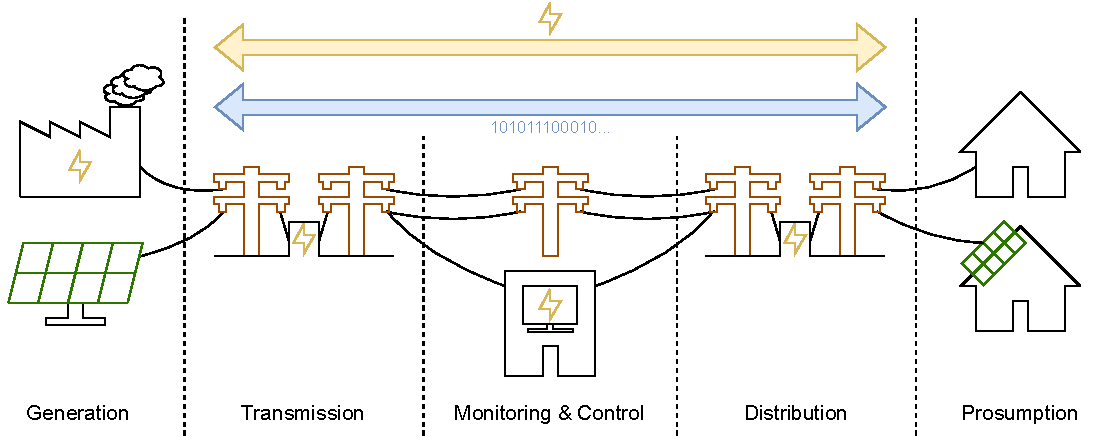
\includegraphics[width=.9\linewidth]{figures/smart_grid_overview_extended_color.drawio.pdf}
    \caption{Bidirectional power and data distribution in a smart electricity grid.}
    \label{fig:smart_grid_overview}
\end{figure}

The IEC 61850 series provides standards for the communication networks of digital energy systems~\cite{IEC61850P5}.
The goals of the IEC 61850 series are seamless communication and interoperability of systems in a smart energy grid.
Although standards for the communication of digital energy systems are provided by the IEC 61850, information security is not an objective of these standards.
To overcome this problem, the IEC 62351 standard series was created by the~\citeauthor{IEC62351P6}.
Part 6 of the IEC 62351 series provides standardized security means for communication compliant to IEC 61850~\cite{IEC62351P6}.
Moreover, Part 8 of the IEC 62351 series provides a role-based access control concept for power systems~\cite{IEC62351P8}.

The focus of this thesis is on the communication aspects of smart grids.
To enhance the communication security and overcome the limitations of existing standards, we propose an approach that can be integrated into smart electricity grids.
The field of application of the approach proposed in this thesis is known as a Substation Automation System (SAS).
A SAS represents the entirety of communication and control equipment of a substation~\cite{Padilla2015}.
A substation is a facility of a high-voltage electricity grid connecting power transmission and distribution lines that use different voltage levels~\cite{oshaSubstation}.
A substation and its SAS represent a specific type of ICS.
The tasks of a SAS are time-critical and have to be executed reliably, as the electricity sector and its substations are critical infrastructures.

\section{Objective}
\label{sec:introduction:objective}
Although standards regarding the communication networks of smart grid systems are widely accepted and utilized, information security continues to confront unresolved challenges.
Historical evidence indicates that economically or politically motivated adversaries pose a risk to OT systems, including energy-related systems.
The \citeauthor{canada2021} \cite{canada2021} published a list of 28 OT-related cybersecurity incidents between 2010 and 2020, including incidents in energy-related sectors.
These incidents comprise 13 state-sponsored incidents, 13 cybercrime incidents, and two incidents perpetrated by thrill-seeking individuals.
The state-sponsored incidents include the Stuxnet malware deployed in Iranian nuclear power and enrichment facilities in 2010 \cite{bbc2010}, the Shamoon malware used against Saudi Aramco in 2012 \cite{reuters2012}, the Blackenergy malware used to attack Ukrainian power distribution systems in 2015 \cite{cisa2021a}, the Industroyer/CrashOverride malware used to shut down remote terminal units of a Ukrainian power transmission facility in 2016 \cite{reuters2016,cisa2021b}, and the Triton/Trisis malware used to attack Triconex Safety Instrumented System (SIS) controllers in 2017 \cite{johnson2017}.
% ...and other incidents in 2013, 2014, 2015, 2017, 2018 as well as 2020 \cite{wsj2015,cisa2018a,bsi2014,hdn2017,vice2017,cisa2018b,toi2020,warrick2020}.

Despite the existence of standards for communication and information security including the IEC 61850 and 62351, there are remaining challenges in order to secure SAS communication.
This thesis focuses on these remaining challenges to enhance the information security of SAS communication.
As stated by \citeauthor{Ishchenko2018} \cite{Ishchenko2018}, these challenges include, among others, ensuring the integrity and authenticity of substation control and protection communication without compromising the time criticality.
For this purpose, cryptographic signature and verification approaches can be employed in the SAS environment.
According to \citeauthor{Elbez2019} \cite{Elbez2019}, the strict time constraints of the low latency communication in substations are key factors for the information security.
Accordingly, Public Key Cryptography (PKC), which was formerly specified by the IEC 62351 standards, seemed to be inappropriate due to computational complexity and latency.

% Based on this proposed approach, the following research questions are going to be answered in the course of this thesis:
Due to an increase in processing performance of IT and OT devices nowadays, this thesis examines the applicability of effective and efficient PKC in substations.
For this purpose, this thesis proposes new cryptographic and cybersecurity approaches for authentication, authorization, and access control.
Moreover, the thesis discusses the employment of speedup techniques to enable the usage of secure PKC in time-critical OT systems.
Therefore, the following research questions are going to be answered in the course of this thesis:
\begin{description}
    \item[RQ1] How can expressive and flexible yet computationally expensive access control approaches such as Attribute-Based Access Control (ABAC) be employed to enable prevention of unauthorized access, enable the Separation of Duties (SoD), and ensure the Principle of Least Privilege (PoLP) in a time-critical SAS environment?
    \item[RQ2] How can a secure and lightweight PKC approach be designed and implemented, that is able to ensure the authenticity, integrity, and non-repudiation of communication in a time-critical SAS environment?
    \item[RQ3] How can authentication, authorization, and access control be integrated into a malleable, scalable, and lightweight cryptosystem for time-critical SAS communication?
\end{description}

\section{Contribution}
\label{sec:introduction:contribution}
With the aim of providing means to enhance the information security in a SAS, we propose a \textbf{C}ertificateless \textbf{A}ttribute-Based \textbf{S}erver-Aided \textbf{C}ryptosystem for \textbf{S}ubstation \textbf{A}utomation \textbf{S}ystems (CASC-SAS).
The main objective of the proposed approach is to provide secure protocols, algorithms, and schemes for SAS communication.
The provided protocols, algorithms, and schemes aim to satisfy SAS security requirements such as integrity, authenticity, access control, and non-repudiation.
Furthermore, the approach takes the specific characteristics, risks, and priorities of OT, ICS, and SAS into account.
To address the aforementioned objectives and considerations, this thesis comprises the following contributions:
\begin{itemize}
    \item Identification of security, safety, availability, performance, and compatibility requirements of the proposed approach, and development of a system model, which represents the corresponding field of application.
    \item Design of a server-aided attribute-based authorization and access control approach, which relies on speedup techniques such as access decision caching and policy evaluation precomputation.
    \item Design of a certificateless attribute-based server-aided authentication approach, which provides algorithm-agnostic cryptographic protocols and services as well as an AB-PKC signature scheme.
    \item Design of a certificateless attribute-based server-aided cryptosystem for SAS, which integrates authentication, authorization, and access control into a dual-path four-layered system architecture.
    \item Implementation of the proposed approach using high-level programming languages, and deployment of the implementation to a test bed that mimics the behavior of an interconnected OT system.
    \item Security evaluation to prove the security characteristics of the approach.
    \item Performance evaluation to demonstrate the applicability of the approach in an OT environment with strict time and resource constraints.
    \item Compatibility evaluation to demonstrate the feasibility of the approach for the construction and retrofitting of a SAS.
\end{itemize}

\section{Structure}
\label{sec:introduction:structure}
The following section presents the structure of this thesis.
The structure consists of six chapters and is illustrated in \autoref{fig:thesis_structure}.

\Cref{ch:introduction} serves to motivate communication security in OT and SAS.
In addition, the chapter presents the research questions and outlines the objective and contributions of the proposed approach.

\Cref{ch:fundamentals} presents the fundamental concepts upon which this thesis and its proposed approach are based.
Among other concepts, it introduces the fundamentals of OT, ICS, information security, system safety, access control, and cryptography.

\Cref{ch:relatedwork} presents a review of the existing literature and offers a delineation between the literature and the proposed approach.

\Cref{ch:approach} defines the proposed SAS security approach, including its system model, requirements, potential adversarial attacks, security policies, security architecture, and realization.
Furthermore, this chapter elucidates the components, algorithms, schemes, and protocols of the proposed security approach.

\Cref{ch:evaluation} presents a comprehensive evaluation of the proposed approach, encompassing security, performance, and compatibility considerations.
Furthermore, the chapter discusses the results of the evaluation, contextualizes the approach within the existing literature by comparing it to related approaches, and describes the limitations and constraints inherent to the evaluation and proposed approach.

In conclusion, \cref{ch:conclusion} provides insight into prospective future research and presents a summary of the thesis.
\begin{figure}
    \centering
    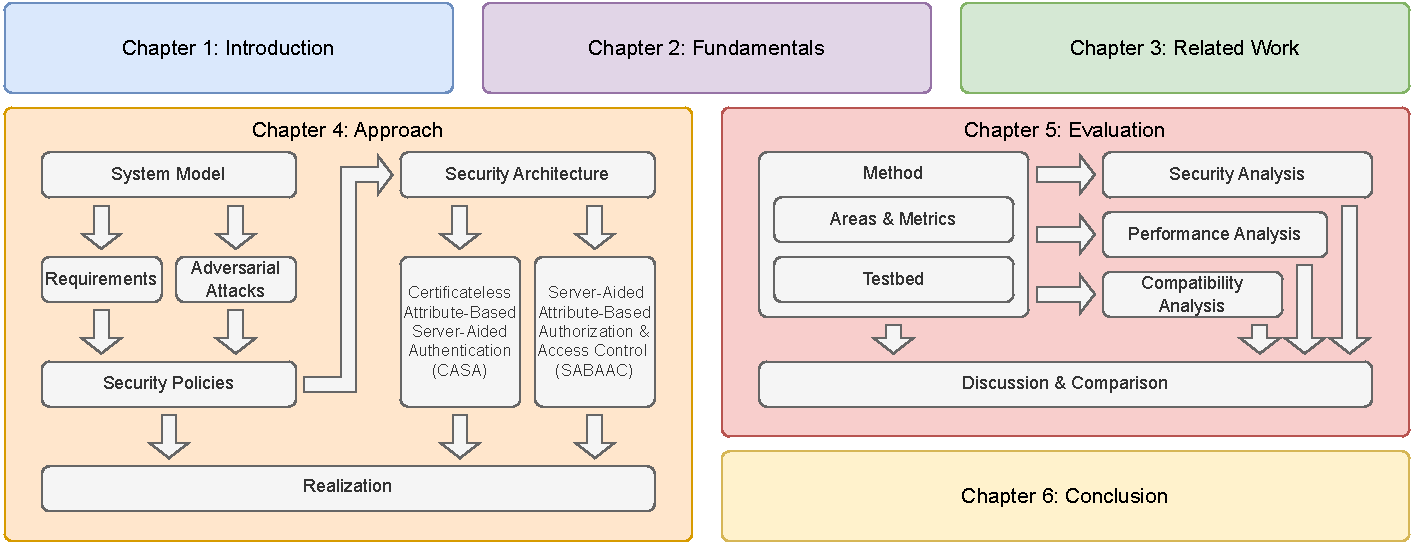
\includegraphics[width=1.\linewidth]{figures/thesis_structure.drawio.pdf}
    \caption{Structure of the thesis consisting of six interrelated chapters.}
    \label{fig:thesis_structure}
\end{figure}

\chapter{Fundamentals}
\label{ch:fundamentals}
The purpose of this chapter is to introduce, define, and describe the fundamental terms and concepts of this thesis proposal.
This chapter provides an introduction for access control in \autoref{sec:accesscontrol}.
Moreover, the relevant fundamentals of cryptography are discussed in \autoref{sec:fundamentals:cryptography}.

\section{Attribute-Based Access Control}
\label{sec:accesscontrol}
Access control is the process of granting and denying specific requests to logical or physical services and resources \cite{NIST2022}.
Based on the type of service or resource guarded by the access control, two types of access control can be distinguished.
Physical access control supervises access requests to physical facilities.
Logical access control supervises the access to information and information processing services.
Within the scope of the thesis proposal, the term access control will be used to describe logical access control for IT and OT systems.

Logical access control protects objects like data, services, executable applications, or network devices from unauthorized operations \cite{Hu2014}.
An operation is performed by a subject on a specific object.
To protect an object, its owners establish access control policies.
These policies describe which subjects may perform certain operations on a specific object.
The policies are enforced by a logical component referred to as Access Control Mechanism (ACM) \cite{Hu2014}.
The ACM receives the access request from a subject, decides whether the request should be granted or denied, and enforces the decision taken.
The ACM takes the decision based on a framework called access control model.
The access control model defines the functionalities and environment including subjects, objects, and rules for the ACM to take and enforce a decision.

Attribute-Based Access Control (ABAC) is an access control model enabling access decisions based on attributes associated with subjects, objects, actions, and the environment of a system \cite{JTF2020}.
In other words, in ABAC an access request of a subject to perform operations on an object is decided based on assigned attributes of the subject and object, environment conditions, and a set of policies \cite{Hu2014}.
Within the context of ABAC, an attribute is a characteristic containing information in the form of a name-value pair \cite{Hu2014}.
A subject attribute such as identity, clearance, or department describes the characteristics of a person or non-person entity.
An object attribute such as the object classification, type, or owner describes the resource for which the access is requested.
An operation or action attribute describes the function performed on an object by a subject.
The environment conditions or environment attributes describe the context of an access request.
Environment conditions include dynamic characteristics like time of the day, day of the week, and request location of the subject.

A policy represents a rule based on which an access decision is taken for specific attributes \cite{Hu2014}.
As a consequence, a policy can be seen as a relationship between subject, object, environment, and operation attributes describing under which circumstances the ACM grants or denies an access request.

Role-Based Access Control (RBAC) and Identity-Based Access Control (IBAC) represent special cases of ABAC regarding their attributes used \cite{Hu2014}.
An advantage of ABAC compared to other access control models is the higher flexibility regarding multifactor policy expression.
Moreover, ABAC can take access control decisions based on ad-hoc knowledge and knowledge from separate infrastructure.
This is possible due to ABAC taking decisions at request time by evaluating policies instead of static decision-making as found in IBAC and RBAC.

\section{Public Key Cryptography}
\label{sec:fundamentals:cryptography}
Cryptography is a scientific discipline concerned with the study of methodologies, algorithms, schemes, and protocols for the encryption and verification of information~\cite{Barker2016,Barker2020,CNSS2022}.
In other words, cryptography provides means to prevent unauthorized access and to enable the verification of information.
The objective of cryptography is to satisfy specific security goals, including the assurance of confidentiality, integrity, authenticity, and non-repudiation.

A cryptographic system or cryptosystem is a set of cryptographic algorithms~\cite{Menezes1996}.
A cryptosystem comprises sets of valid inputs and outputs as well as required cryptographic keys~\cite{Eckert2023}.
Two important principles for the design of cryptosystems were formulated by \citeauthor{Kerckhoffs1883} and \citeauthor{Shannon1949}.
As stated by \citeauthor{Kerckhoffs1883}, the cryptosystem must not require secrecy and must be able to be known by the adversary without inconvenience~\cite{Kerckhoffs1883}.
According to \citeauthor{Shannon1949}, it shall be assumed that the adversary knows the system being used~\cite{Shannon1949}.
The goal of a cryptosystem is to provide specific cryptographic services such as encryption or verification.
Verification describes the process of proving the integrity, authenticity, or non-repudiation of information~\cite{Boneh2023}.
The verification of information is based on a so-called tag or signature created by a signature algorithm.
Encryption describes the process of transforming plain information called plaintext into an unintelligible form called ciphertext to maintain its secrecy~\cite{Barker2016,Boneh2023}.
The inverse process of encryption is referred to as decryption.

Public Key Cryptography (PKC), also referred to as asymmetric cryptography, relies on algorithms which use a pair of two related keys for a cryptographic operation and its inverse operation~\cite{Barker2020,CNSS2022,Eckert2023}.
The pair of related keys in PKC consists of a private key, which must be kept secret, and a public key, which may be shared without consequences for security, as long as its authenticity and integrity is ensured.
In contrast to PKC, secret-key or symmetric cryptography uses the same key for a cryptographic operation and its inverse operation.

PKC offers the following advantages over symmetric cryptography~\cite{Barker2020,Eckert2023}:
Firstly, PKC does not require a secure channel or secure protocol to exchange keys.
Secondly, the overall number of required keys using PKC is lower.
Moreover, the number of keys scales linear with the number of communication entities.
For example in a network with $n$ entities, $n$ key pairs or $2n$ keys have to be established.
In the same network, pairwise symmetric cryptography would require $n(n-1)/2$ keys.

Nevertheless, symmetric cryptography has advantages in comparison with asymmetric cryptography~\cite{Barker2020}.
Firstly, symmetric-key algorithms are faster than asymmetric-key algorithms.
Secondly, for a given level of security, symmetric cryptographic keys are shorter.
This reduces the memory and bandwidth requirements for key storage and transmission.

\subsection{Certificateless Public Key Cryptography}
Certificateless Public Key Cryptography (CL-PKC) can be seen as an intermediate approach between Identity-Based Public Key Cryptography (ID-PKC) and certificate-based PKC approaches such as Public Key Infrastructure (PKI)~\cite{AlRiyami2003}.
CL-PKC approaches make use of a Trusted Third Party (TTP) called Key Generating Center (KGC) to generate partial private keys based on an entity's identity and a master key.
To obtain the private key, the entity combines the partial private key with a secret value.
Consequently, CL-PKC neither suffers from the key escrow problem nor requires a secure communication channel for the key distribution.
To obtain the public key, the entity generates it based on public parameters and the secret value.
Similar to ID-PKC, the public key is not derived from the private key and may therefore exist prior to it.
The only restriction is that the public key and the private key must use the same secret value.

\subsection{Attribute-Based Public Key Cryptography}
Attribute-Based Public Key Cryptography (AB-PKC) is a generalization of the ID-PKC concept~\cite{Sahai2005,Goyal2006,Hu2023}.
Attribute-Based Encryption (ABE) combines the principles of ABAC with the concept of PKC.
Therefor, attribute-based policies are integrated into cryptographic algorithms in the form of access structures and attributes.
ABE approaches are classified as either Key-Policy ABE (KP-ABE) or Ciphertext-Policy ABE (CP-ABE), depending on whether the access structure is associated with a key or a ciphertext~\cite{Goyal2006,Bethencourt2007,Hu2023}.
In KP-ABE a secret key is able to decrypt a ciphertext if the attributes of the ciphertext satisfy the key-associated access structure.
Consequently, a data owner cannot control who is able to access the data and has to trust a TTP to issue appropriate keys~\cite{Bethencourt2007}.
In CP-ABE a secret key is able to decrypt a ciphertext if the key-associated attributes satisfy the ciphertext's access structure.
Accordingly, each data owner manages the access control policies for its own data, which makes CP-ABE more flexible and scalable than KP-ABE.
Similar to the concept of ABE, Attribute-Based Signatures (ABS) enable the integration of attributes into signing and verification algorithms~\cite{Li2010,Maji2011}.

\chapter{Related Work}
\label{ch:relatedwork}
%%% Ishchenko2018 - Secure Communication of Intelligent Electronic Devices in Digital Substations
An authenticated communication approach for network packets between IEDs and merging units is presented by \citeauthor{Ishchenko2018} \cite{Ishchenko2018}.
They introduce a system and bump-in-the-wire device called security filter as an add-on device between IEDs and Ethernet-based communication busses using the Generic Object Oriented Substation Event (GOOSE) or Sampled Values (SV) protocol.
Security filter appends Message Authentication Code (MAC) tags to outgoing messages of the IEDs and verifies incoming MAC tags.
As a consequence, the communication busses are secured against unauthenticated messages achieving the security goals integrity and authenticity.
The authors showed that the security filter is able to meet the IEC 61850 performance requirements of GOOSE and SV \cite{IEC61850P5} using a HMAC and GMAC algorithm even on commodity of-the-shelf ARM hardware.

%%% Elbez2019 - Authentication of GOOSE Messages under Timing Constraints in IEC 61850 Substations (10.14236/ewic/icscsr19.17)
A review of IEC 62351 security recommendations with regard to message authentication and a comparison of viable authentication approaches for IEC 61850 substations is presented by \citeauthor{Elbez2019} \cite{Elbez2019}.
The authors implemented a digital signature authentication scheme and a keyed Hash Message Authentication Code (HMAC) scheme for GOOSE messages and compared the required computational times.
According to the authors, the computational times show that asymmetric cryptography solutions based on RSA and RSASSA-PSS are not suitable for the timing constraints of GOOSE messages.
In contrast, the authentication time of the HMAC approach is of the order of microseconds, making it a more viable approach for the substation domain.

%%% Rodriguez2021 - A Fixed-Latency Architecture to Secure GOOSE and Sampled Value Messages in Substation Systems
An authentication and encryption approach for substation communication using the protocols GOOSE and SV is presented by \citeauthor{Rodriguez2021} \cite{Rodriguez2021}.
The authors present a hardware architecture for the encryption and authentication of GOOSE and SV packets at wire-speed conforming to IEC 62351:2020~\cite{IEC62351P6}.
The hardware implementation is able to process GOOSE and SV packets with a fixed latency in the order of microseconds.
Consequently, the authors state that the presented hardware architecture is able to provide integrity and confidentiality without exceeding the maximum delivery time of three milliseconds introduced by IEC 61850 for GOOSE and SV packets~\cite{IEC61850P5}.

%%% Hong2019 - Cyber Attack Resilient Distance Protection and Circuit Breaker Control for Digital Substations
To protect substations against attacks, \citeauthor{Hong2019} \cite{Hong2019} present a domain-based collaborative mitigation approach.
According to the authors, the goal of the approach is to enable substation devices to collaboratively defend against attacks.
The authors present three attack scenarios that can be mitigated using the presented domain-based collaborative approach.
The presented attack scenarios are an accidental or malicious IED configuration change, false sensor data injection, and false device command injection.
Collaborating devices can block these attacks by validating sensor data and configuration changes based on measurements and metrics as well as predicting consequences of control actions.

%%% Ruland2018 - Firewall for Attribute-Based Access Control in Smart Grids (10.1109/SEGE.2018.8499306)
An access control approach driven by ABAC policies for smart grid systems including substations is presented by \citeauthor{Ruland2018} \cite{Ruland2018}.
The presented access control approach is realized in the form of an access control firewall.
The access control firewall splits the station bus into an inner and an outer region and connects these regions by processing access requests of connected devices.
The inner station bus connects IEDs and enables low-latency GOOSE or GSSE communication between them.
The access control firewall enforces access request decisions based on ABAC policies.

%%% Burmester2013 - T-ABAC: An attribute-based access control model for real-time availability in highly dynamic systems (10.1109/ISCC.2013.6754936)
A real-time capable ABAC approach is presented by \citeauthor{Burmester2013} \cite{Burmester2013}.
The authors propose an extended ABAC model that is based on time-dependent attributes to support availability within the strict time constraints of cyber-physical systems.
The availability of a time-dependent attribute can be expressed with an availability label that is dynamically determined based on user and system events as well as the context of the requested service.
The authors demonstrate the real-time ABAC approach for IP multicast in Trusted Computing (TC) compliant networks.

%%% Lee2015 - Role-based access control for substation automation systems using XACML (10.1016/j.is.2015.01.007)
An IEC 61850 and IEC 62351 compliant RBAC approach for substations is presented by \citeauthor{Lee2015} \cite{Lee2015}.
The approach focuses on session-based access control for TCP/IP communication on the station bus of substations.
The presented implementation relies on a role-based client-server architecture.
The implementation demonstrates the feasibility of RBAC for substations as specified by IEC 62351~\cite{IEC62351P8}.
Furthermore, the presented implementation is capable of processing and responding to MMS requests within the 500 millisecond time requirement for type 3 messages (low speed messages) specified by IEC 61850-5~\cite{IEC61850P5}.

%%% Ma2006 - Constraint-Enabled Distributed RBAC for Subscription-Based Remote Network Services (10.1109/CIT.2006.63)
A distributed RBAC approach for subscription-based remote network services is presented by \citeauthor{Ma2006} \cite{Ma2006a,Ma2006}.
The authors propose a distributed authentication and role-based authorization framework called Distributed Role-based Access Control (DRBAC).
The distributed authentication is realized by delegating the authentication of users to their subscribing institutions by issuing authentication delegation certificates.
The role-based authorization approach extends traditional RBAC by adding the concept of distributed roles shared by the service provider and service subscribers.
This enables access control policies associated with distributed roles rather than subject identities, which leads to an increase in scalability and manageability of access control.
Moreover, the authors state that their DRBAC approach supports temporal, contextual, or cardinality constraints to enhance the semantic expressiveness of access control and enable the definition of higher-level organizational policies.

%%% Alcaraz2016 - Policy enforcement system for secure interoperable control in distributed Smart Grid systems (10.1016/j.jnca.2015.05.023)
A rule-based RBAC policy enforcement approach for smart grid systems is presented by \citeauthor{Alcaraz2016} \cite{Alcaraz2016}.
The presented approach integrates into a smart grid system with supernode networking architecture.
Supernodes are servers at fixed locations responsible for handling data flows of a set of subscribers~\cite{Samuel2008}.
The policy enforcement approach presented by \citeauthor{Alcaraz2016} consists of three execution phases, namely authentication, authorization, and interoperability.
The approach is based on a rule-based expert system and a context manager for the analysis of the subject, target object, and context of a request.

\chapter{Approach}
\label{ch:approach}
In the following section, we introduce our proposed security approach for substation automation systems.
With the aim of securing the time-critical communication between resource-constrained devices in a time-variable environment, we propose a \textbf{C}ertificateless \textbf{A}ttribute-Based \textbf{S}erver-Aided \textbf{C}ryptosystem for \textbf{S}ubstation \textbf{A}utomation \textbf{S}ystems (CASC-SAS).
The CASC-SAS cryptography and cybersecurity approach is able to prevent and mitigate cyberattacks by providing security schemes and mechanisms, and enforcing mandatory communication policies.
The goal of the approach is the enhancement of SAS security by providing secure authentication, authorization, and attribute-based access control for time-critical SAS communication.

The CASC-SAS approach comprises two core concepts.
The first core concept of the approach is the \textbf{C}ertificateless \textbf{A}ttribute-Based \textbf{S}erver-Aided \textbf{A}uthentication (CASA).
This concept represents the foundation of the CASC-SAS approach.
The concept provides cryptographic algorithms and schemes for authentication, including a PKC signature scheme for key generation, signing, and verification.
Communicating SAS devices as well as more abstract cybersecurity services can rely on the provided communication integrity, authenticity, and non-repudiation.
The CASA concept is further discussed in \autoref{sec:approach:casa}.
The second core concept of the approach is the \textbf{S}erver-Aided \textbf{A}ttribute-\textbf{B}ased \textbf{A}uthorization and \textbf{A}ccess \textbf{C}ontrol (SABAAC).
This concept provides mechanisms to enable attribute-based authorization and ABAC for time-critical SAS communication.
Accordingly, this concept represents cybersecurity means to provide access control, PoLP, and SoD.
For this purpose, the concept relies on authentication services provided by CASA.
The SABAAC concept is further discussed in \autoref{sec:approach:sabaac}.

In the following sections, we introduce and discuss our proposed approach.
At the beginning of this chapter, in \autoref{sec:approach:system_model}, we discuss the field of application of the proposed approach by introducing a system model.
Based on the presented system model, we define the requirements of the proposed approach in \autoref{sec:approach:requirements}.
In \autoref{sec:approach:attacks} we address potential adversarial attacks, for which the approach must provide mitigation strategies.
To satisfy the aforementioned requirements and mitigate adversarial attacks, the CASC-SAS approach enforces security policies, which are discussed in \autoref{sec:approach:security_policies}.
Subsequently, in \autoref{sec:approach:casc:architecture}, the dual-path four-layered security architecture of CASC-SAS is defined.
The two main CASC-SAS concepts, its cryptography approach CASA and its authorization and access control approach SABAAC, are introduced in \autoref{sec:approach:casa} and \autoref{sec:approach:sabaac}.
Finally, in \autoref{sec:approach:realization}, we present the realization of the CASC-SAS approach.
% Subsequently, we present the proposed evaluation strategies and metrics of the approach in \autoref{sec:approach:evaluation}.
% Finally, in \autoref{sec:approach:limitations} we discuss limitations of the proposed approach.

\section{System Model}
\label{sec:approach:system_model}
In the following sections, we introduce the system model of the CASC-SAS approach.
The system model serves the purpose of delimiting the scope and area of application of the proposed approach.

The area of application of the proposed approach consists of ICSs in the power system domain.
More specifically, the proposed approach is tailored to the communication and control systems of substations in the electricity grid.
The communication and control equipment of an ICS is referred to as secondary equipment.
The entirety of secondary equipment of a substation is referred to as SAS \cite{Padilla2015}.
Although the proposed approach is tailored to the power system domain and substation environment, its main concepts may also be applied to other ICSs with similar requirements and constraints.

\subsection{Architecture}
The architecture of the presented system model is based on the IEC 61850 standards \cite{IEC61850P5}.
The presented system model architecture consists of four layers called network, station, bay, and process level.
The process, bay, and station level represent the internal layers of a SAS architecture.
The SAS architecture containing the three internal layers as well as the station and process bus is shown in \autoref{fig:substation_architecture}.
The shown busses are further discussed in \autoref{sec:approach:system_model:communication}.
The network level represents a SAS-external layer to integrate multiple SAS instances and supervisory controllers into a comprehensive power system.
Each of the four layers consists of different devices and provides different control and automation functions:
\begin{enumerate}
    \item Process Level: The process level provides functions to interact with the physical process via sensors and actuators.
    As a consequence, SAS devices located at the process level provide interfaces to the physical process.
    In other words, devices located at the process level transform analog measurements or control signals into digital values and vice versa.
    Devices restricted to the transformation and provision of measurement and control values are referred to as Merging Units (MU).
    Moreover, IEDs can be employed at the process level to combine MU functions with higher-level functions such as protection or communication tasks.

    \item Bay Level: The bay level provides common functions of so-called bays of a SAS.
    As stated by the \citeauthor{IEC61850P5} \cite{IEC61850P5}, a bay represents a closely connected subpart of a substation with common functionality.
    The devices at bay level supervise the operation of lower-level devices of a SAS bay.
    Consequently, a supervising bay level device is referred to as bay controller or bay protection.

    \item Station Level: The station level provides functions related to the substation as a whole.
    Therefore, the station level comprises devices required for on-site and remote monitoring and control of the substation.
    Devices at the station level include Human Machine Interfaces (HMI) for substation operators as well as Wide Area Network (WAN) gateways like SCADA RTUs.

    \item Network Level: The network level provides higher-level functions exceeding the scope of a single SAS.
    The network level devices include supervisory monitoring and control devices like SCADA MTUs.
\end{enumerate}
\begin{figure}
    \centering
    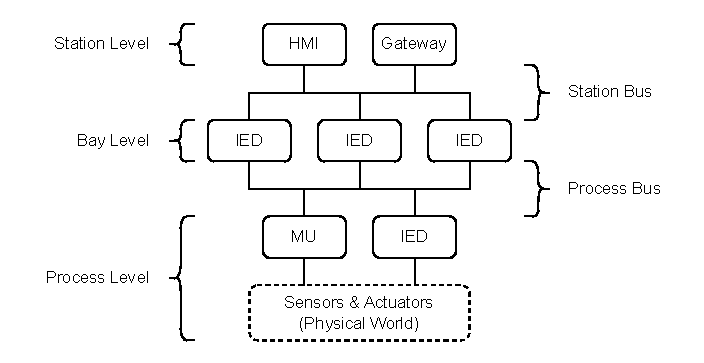
\includegraphics[width=1.0\linewidth]{figures/substation_architecture.drawio.pdf}
    % \caption{The internal SAS architecture consisting of three layers called system level, bay level, and process level which are connected via station bus and process bus.}
    \caption{Internal three-layered architecture of a SAS.}
    \label{fig:substation_architecture}
\end{figure}

\subsection{Communication}
\label{sec:approach:system_model:communication}
In the following, we discuss the communication between devices of the presented system model.
For this purpose, we identify different communication characteristics based on which communication relationships and messages can be classified.
Moreover, we define three messages types for time-critical ICS and SAS communication.
Furthermore, we discuss the bus-based device interactions occurring in the above-mentioned four layer system model.

\subsubsection{Classification Characteristics}
The communication relationships between devices within a SAS can be classified using different communication characteristics.
In the following sections, classifications based on topology, continuity, and latency are further discussed.

\paragraph{Topology-Based Classification}
Topological communication characteristics can be used to classify the device relationships based on their relative or absolute location within the system model.
Accordingly, communication can either occur between devices on the same layer or different layers of the system model.
Communication on the same layer of the system model is referred to as horizontal communication, whereas communication between devices on different layers is referred to as vertical communication.
Moreover, communication can occur between devices of the same or different subsystems.
Communication between devices of the same subsystem is classified as internal communication, whereas communication relationships including an external device are classified as external communication.
Furthermore, a communication relationship is not limited to a single receiver using unicast, but rather a group of devices via multicast or all devices via broadcast may receive a sender's message.

\paragraph{Continuity-Based Classification}
Besides the topology-based classification, communication relationships can be classified based on their continuity.
Continuous, session-oriented, or stateful communication requires an initial session establishment between the involved devices.
While the first message exchange requires additional initialization overhead, subsequent latencies may benefit from the established communication session.
Discontinuous, message-oriented, or stateless communication enables communication without initial overhead for the involved devices.
Consequently, discontinuous communication does not lead to latency emerging from session initialization and management.

\paragraph{Latency-Based Classification}
Since communication in ICS and SAS is time-critical, communication relationships can be classified based on their communication latency constraints.
Within the scope of the proposed approach, we define communication latency as sum of processing time and transmission time required to exchange information between involved devices.
As a consequence, the communication latency represents the time an individual message requires to be delivered from the sending buffer of a host to the receiving buffer of another host.

Transmission time is the time required to transmit a message over a network link with a specific throughput, whereas processing time represents the time required for a device to send, forward, or receive a message.
For intermediate network devices like routers and switches the processing time depends on queuing delay and forwarding delay.
For the sender and receiver of a message the processing time consists of enqueue and dequeue delays, cryptographic overhead, and message coding.

To support Ethernet-based SAS protocols such as GOOSE and SV, communication latency constraints for each individual data frame of the data link layer must be taken into account.
The composition of the end-to-end latency of Ethernet-based communication is visualized in \autoref{fig:frame_delivery_time_composition}.
In \autoref{fig:frame_delivery_time_composition:unverified}, the communication latency is composed of time for encoding ($t_{E}$), time for transmission to another host or intermediate system ($t_{T}$), time for switching in an intermediate system ($t_{S}$), and time for decoding ($t_{D}$).
In \autoref{fig:frame_delivery_time_composition:verified}, device-local data verification is employed, which leads to additional processing time required for signing ($t_{Sig}$) and verification ($t_{Ver}$).
\begin{figure}
    \centering
    \begin{subfigure}[t]{0.85\linewidth}
        \centering
        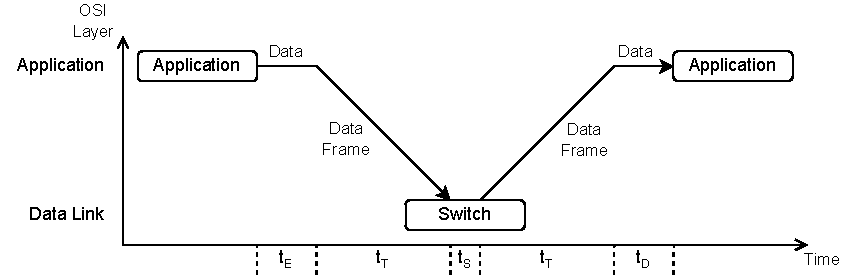
\includegraphics[width=\linewidth]{figures/frame_delivery_time_without_signature.drawio.pdf}
        \caption{No data verification.}
        \label{fig:frame_delivery_time_composition:unverified}
        \vspace{1.0\baselineskip}
    \end{subfigure}
    \begin{subfigure}[t]{0.85\linewidth}
        \centering
        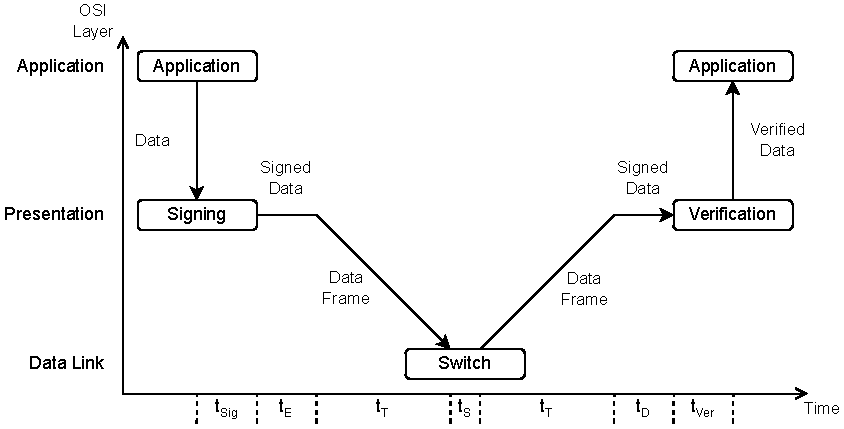
\includegraphics[width=\linewidth]{figures/frame_delivery_time_with_signature.drawio.pdf}
        \caption{Device-local data verification.}
        \label{fig:frame_delivery_time_composition:verified}
    \end{subfigure}
    \caption{Composition of the end-to-end latency using Ethernet-based communication.}
    \label{fig:frame_delivery_time_composition}
\end{figure}

\subsubsection{Message Types}
\label{sec:approach:system_model:communication:message_types}
The defined message types of the presented system model are based on the classification characteristics defined above.
Furthermore, the defined message types have been adapted from the message types and performance classes of the IEC 61850 standards \cite{IEC61850P5}.
The defined message types as well as their typical communication topology, continuity, and latency constraints are shown in \autoref{tab:message_types}.

The low latency message type corresponds to the IEC 61850 \cite{IEC61850P5} message types 1A and 4.
These messages are used for SAS-internal exchange of sampled values and state values.
In IEC-compliant substations, the sampled values are exchanged via multicast using the SV protocol between MUs and IEDs (vertical) or between MUs (horizontal).
Moreover, state values and state changes are exchanged between IEDs (horizontal) using the GOOSE protocol.

The medium latency message type corresponds to the IEC 61850 message types 1B and 2.
These messages are used for SAS-internal and SAS-external, as well as horizontal and vertical session-based client-server communication.
In IEC-compliant substations, IEDs use the MMS protocol to communicate with other IEDs and higher-level devices.

The high latency message type corresponds to the IEC 61850 message types 3 and 5.
This message type is used for HMI interactions as well as non-time-critical operations like file transfers.
In IEC-compliant substations, MMS as well as SCADA protocols are used for high latency communication.
\begin{table}
    \centering
    \small
    % \caption{Message types of the presented system model classified with regard to their topology, continuity, and latency constraints of the communication relationships.}
    \caption{Message types of the presented system model.}
    \label{tab:message_types}
    \begin{tabular}{l c c c c c}
    \toprule
    \multicolumn{1}{c}{Message Type} & \multicolumn{3}{c}{Topology} & Continuity & Latency\\
    \cmidrule(lr){2-4}
    & Externality & Verticality & Receiver & & Constraint\\
    \midrule
    Low Latency & Internal & Horiz./Vert. & Multicast & Message-Based & 3 ms\\
    Medium Latency & Int./Ext. & Horiz./Vert. & Unicast & Session-Based & 20-100 ms\\
    High Latency & Int./Ext. & Horiz./Vert. & Unicast & Session-Based & 500 ms\\
    \bottomrule
    \end{tabular}
\end{table}

\subsubsection{Communication Buses}
The presented system model uses a bus-based approach for message exchange within and between the system architecture layers.
The realization of SAS-internal buses is typically based on Ethernet, and on open or proprietary fieldbus technology.
The bus-based approach as well as the two specific buses introduced in the following are based on the IEC 61850 standards \cite{IEC61850P5}.

The first bus for SAS-internal message exchange is referred to as process bus.
The process bus is located between the bay level and the process level.
The process bus is used for time-critical message-based publisher-subscriber communication, i.e., multicast or broadcast communication.
GOOSE and SV are the protocols used for process bus communication.

The second bus for SAS-internal message exchange is referred to as station bus.
The station bus is located between the station level and the bay level.
The station bus connects IEDs at the bay level with each other as well as with gateways and interfaces at the station level.
The communication at the station bus is typically session-based unicast communication with less strict time requirements compared to the process bus.

SAS-external message exchange between devices on the station level and network level use WAN telecommunication technologies including Internet, satellite, cellular, and radio technology.
Secure tunneling approaches like Virtual Private Networks (VPN) can be used to enhance the security of SAS message exchange over an unsecure communication medium.

\section{Requirements}
\label{sec:approach:requirements}
In the following, we introduce the requirements of the presented approach.
Based on the identified requirements, functional and non-functional characteristics of the proposed approach are derived and evaluated.
Each requirement is associated with a requirement category.
We define five requirement categories for the introduced system requirements.
The requirement categories consist of security (RQ.SEC), safety (RQ.SAF), availability (RQ.AVA), performance (RQ.PER), and compatibility (RQ.COM).

\subsection{Security}
\begin{description}
    %\paragraph{RQ.SEC.1 Confidentiality}
    %The system prohibits unauthorized access to sensitive information stored on devices and payload of messages exchanged within the system and between systems \cite{Eckert2023}.
    \item[RQ.SEC.1] Data Frame Payload Integrity\\
    A SAS device detects unauthorized manipulation of data frames that are exchanged between itself and another device.
    \item[RQ.SEC.2] Data Frame Sender Authenticity\\
    Each SAS device can prove the authenticity and trustworthiness of a sender of a data frame.
    \item[RQ.SEC.3] Data Frame Authorship Non-Repudiation\\
    A SAS device cannot dispute its authorship of a data frame sent.
    \item[RQ.SEC.4] Access Control\\
    The system prohibits unauthorized access to sensitive information stored on devices.
    \item[RQ.SEC.5] Principle of Least Privilege  (PoLP)\\
    The system ensures that each subject has the least number of privileges necessary to perform its function \cite{JTF2020}.
    \item[RQ.SEC.6] Separation of Duties (SoD)\\
    The system ensures that no subject has enough privileges to be able to misuse the system without collusion \cite{JTF2020}.
    %\paragraph{RQ.SEC.7 Privacy Preservation}
    %\todo{TODO: Does this conflict with the idea of proving the origin of a request? In other words, is it possible to check if the subject who requested the access decision is still the same subject who used it in its request?}
\end{description}

\subsection{Safety}
\begin{description}
    \item[RQ.SAF.1] Safe Operation\\
    Under possible operating conditions, the system must not pose a threat to itself and its environment.
    \item[RQ.SAF.2] Fail-Safe\\
    In case of failure, the system terminates without causing harm to the system or system environment~\cite{rfc4949}.
    In other words, the system never transitions into an unsafe state.
\end{description}

\subsection{Availability}
\begin{description}
    \item[RQ.AVA.1] Continuing Operation\\
    Under possible operating conditions, the system must continue its operation as stated by the system requirements.
    \item[RQ.AVA.2] Fail-Operational\\
    In case of failure, the system aims to continue its operation by selectively terminating failing system functions.
    The selective termination of non-essential system functions in case of a failure is also referred to as fail-soft~\cite{rfc4949}.
\end{description}

\subsection{Performance}
\begin{description}
    \item[RQ.PER.1] Constrained Data Frame Delivery Time\\
    The latency constraints for network communication, as defined in \autoref{sec:approach:system_model:communication:message_types}, must be satisfied.
    To support Ethernet-based SAS protocols, the approach must be able to satisfy time constraints for each individual data frame of the data link layer.
    \item[RQ.PER.2] Constrained Computational Performance\\
    The limited performance of resource-constrained devices of an SAS must be taken into account.
    Consequently, computationally complex algorithms must be executed by performance-oriented TTPs.
    \item[RQ.PER.3] Constrained Energy \& Power\\
    The limited energy and power of resource-constrained devices of an SAS must be taken into account.
    Consequently, energy-intensive tasks, such as long-running computations, or power-intensive tasks, such as tasks leading to high CPU loads, must be executed by performance-oriented TTPs.
\end{description}

\subsection{Compatibility}
\begin{description}
    \item[RQ.COM.1] Interoperability\\
    The system components are capable of exchanging information and providing services, irrespective of whether they originate from a single vendor or multiple vendors~\cite{IEC61850P5}.
    \item[RQ.COM.2] Interchangeability\\
    The system's behavior and functionality may not be influenced by an exchange of devices with an equal range of functions from a single vendor or multiple vendors~\cite{IEC61850P5}.
\end{description}

\section{Adversarial Attacks}
\label{sec:approach:attacks}
In addition to the aforementioned requirements, this section introduces an adversary model and provides an enumeration and classification of cyberattacks.
While not being exclusively relevant to SAS, the presented adversaries and attacks pose a threat to the state and operation of systems that correspond to the system model defined in \autoref{sec:approach:system_model}.
A plethora of different threats, adversaries, and cyberattack classifications applicable to SCADA, SAS, ICS, or smart grid systems are discussed in the literature \cite{Nicholson2012,Aloul2012,Rizzetti2015,Youssef2016,Cai2016,Hussain2021}.
In the following paragraphs, these concepts are aggregated and transferred to the area of application of the CASC-SAS approach.

For the purpose of design, realization, and evaluation of the CASC-SAS approach, we assume an adversary corresponding to the Dolev-Yao model \cite{Dolev1983}.
The Dolev-Yao adversary is adapted to the SAS-specific network characteristics, including the usage of two separated buses for the exchange of messages.
Based on the adversary classification presented by \citeauthor{Hof2007} \cite{Hof2007} and \citeauthor{Ponikwar2016} \cite{Ponikwar2016}, the defined Dolev-Yao-like CASC-SAS adversary is a malicious, global, cooperative, dynamic, active, insider adversary.
Accordingly, a possible CASC-SAS adversary is characterized by five assumptions:
\begin{enumerate}
    \item The adversary has physical or remote access to at least one of the internal SAS networks, i.e., the process bus or the station bus.
    \item The adversary is able to initiate arbitrary message exchanges with any device on the networks.
    \item The adversary is able to receive messages from any device on the networks.
    \item The adversary is able to capture, alter, and drop messages exchanged on the networks.
    \item The adversary is unable to bypass or break cryptographic procedures without first obtaining the necessary key material.
\end{enumerate}

The types of cyberattacks that a CASC-SAS adversary can carry out are visualized in \autoref{fig:attack_classification}.
Each cyberattack is classified based on the security objective affected.
The objective of availability-focused attacks, as illustrated in \autoref{fig:attacks_availability}, is to disrupt system services in a manner that renders the continuation of operations impossible.
In contrast, integrity-focused attacks, as illustrated in \autoref{fig:attacks_integrity}, aim to disturb the system's integrity by transitioning the system into a state that is either invalid or beneficial for an adversary.
The authenticity-focused attacks shown in \autoref{fig:attacks_authenticity} enable an adversary to impersonate a legitimate subject of the system, thereby abusing the subject's granted privileges.
\begin{figure}
    \centering
    \begin{subfigure}[t]{0.38\linewidth}
        \centering
        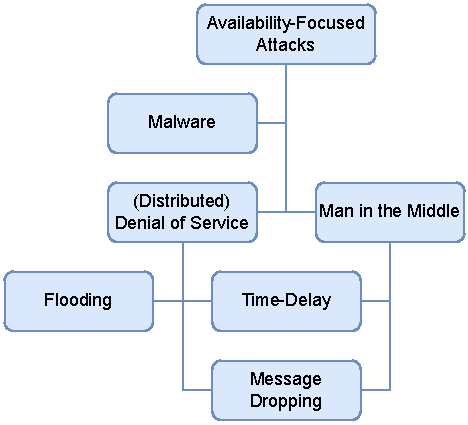
\includegraphics[width=\linewidth]{figures/attacks_availability.drawio.pdf}
        \caption{Availability-focused attacks.}
        \label{fig:attacks_availability}
    \end{subfigure}
    \hfill
    \begin{subfigure}[t]{0.295\linewidth}
        \centering
        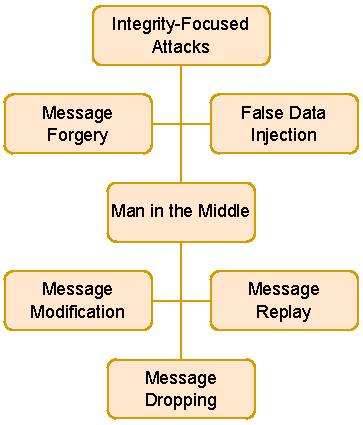
\includegraphics[width=\linewidth]{figures/attacks_integrity.drawio.pdf}
        \caption{Integrity-focused attacks.}
        \label{fig:attacks_integrity}
    \end{subfigure}
    \hfill
    \begin{subfigure}[t]{0.30\linewidth}
        \centering
        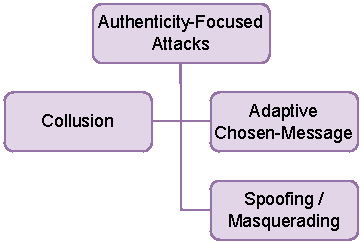
\includegraphics[width=\linewidth]{figures/attacks_authenticity.drawio.pdf}
        \caption{Authenticity-focused attacks.}
        \label{fig:attacks_authenticity}
    \end{subfigure}
    \caption{Classification of adversarial attacks based on security objectives.}
    \label{fig:attack_classification}
\end{figure}

In addition to the classification based on the affected security objective, we propose a classification of potential cyberattacks based on the adversary's objective.
These objectives are modeled as attack trees, as the objective of an adversary is typically unachievable by a single operation but rather requires a sequence of attacks to be achieved.
This modeling approach allows for a more comprehensive understanding of the adversary's strategy and the potential avenues for defense.
With regard to the CASC-SAS approach, two primary objectives of an adversary were identified.
The first objective is an attack against the SAS network communication, i.e., against the SAS protocols.
The second objective is an attack against SAS devices.
Accordingly, two independent attack trees are provided in \autoref{fig:attack_tree_communication} and \autoref{fig:attack_tree_device}.
The colors utilized for the visualization of attacks within the attack trees correspond to the colors utilized in \autoref{fig:attack_classification} and, thus, represent the affected security objective.

The first attack tree, as illustrated in \autoref{fig:attack_tree_communication}, represents an adversary with the objective of compromising the system by disrupting communication between two or more legitimate system subjects.
In order to achieve this objective by compromising the communication integrity, the adversary may either replay messages that have been captured on the network, or modify them.
While replaying only requires the adversary to be able to eavesdrop on communication, message modification additionally requires the adversary to masquerade as a legitimate subject.
This can be achieved by either breaking authenticity and integrity protection mechanisms, such as digital signatures, or colluding with other adversaries, such as infiltrated system devices.
Furthermore, an adversary may disrupt communication via (distributed) denial of service (DoS) attacks.
Examples of DoS attacks in a SAS include the intentional delay of time-critical messages, also known as time-delay attacks \cite{Bianchin2018}, and dropping of messages.
\begin{figure}
    \centering
    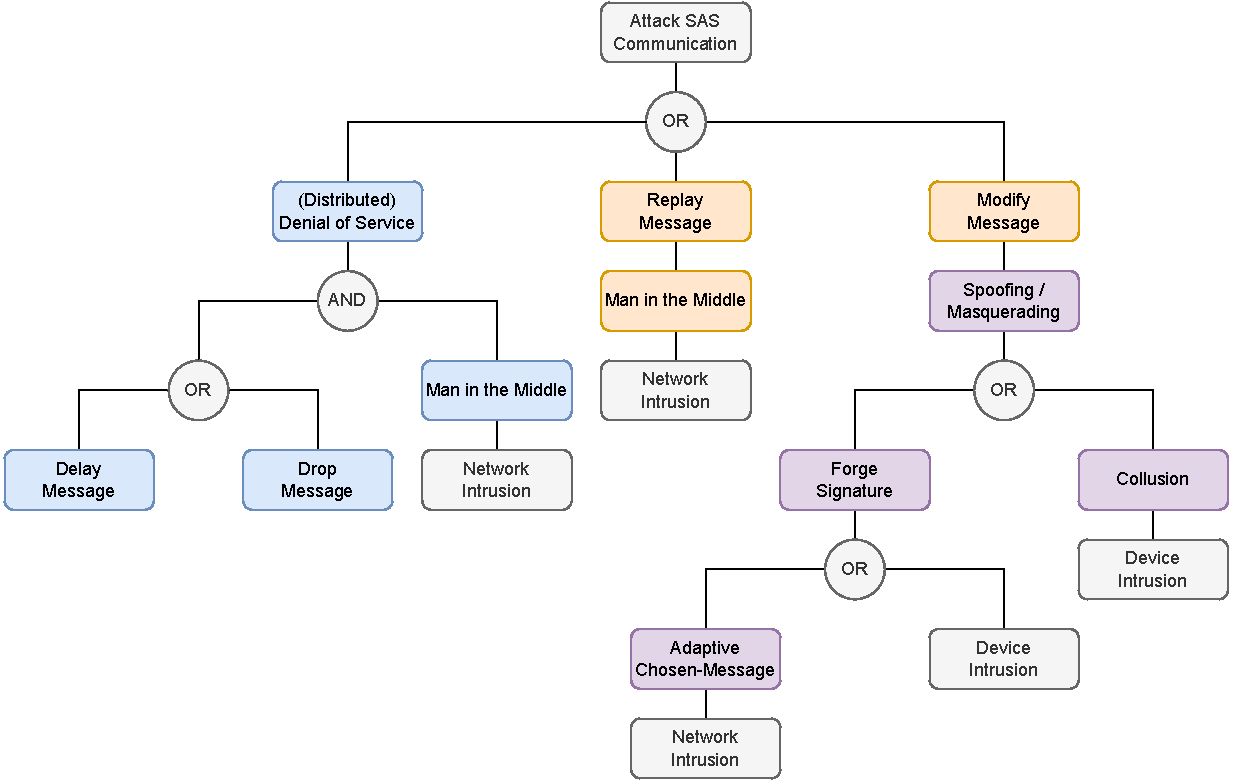
\includegraphics[width=1.0\linewidth]{figures/attack_tree_communication.drawio.pdf}
    \caption{Attack tree comprising cyberattacks that endanger SAS message exchange protocols.}
    \label{fig:attack_tree_communication}
\end{figure}

The second attack tree, as illustrated in \autoref{fig:attack_tree_device}, represents an adversary with the objective of compromising the system by directly attacking the system devices.
An adversary may seek to either disrupt the device's availability or compromise its integrity.
An adversary may achieve disruption of the device's availability via the deployment of malware or (distributed) DoS attacks, such as flooding attacks.
A device's integrity can be compromised by modifying its state using accessible service interfaces.
Consequently, an adversary may either create a legitimate request, in case of an unsecured service, or forge a request.
As discussed above with regard to message modification, request forgery might require an adversary to masquerade as a legitimate subject to circumvent authenticity and integrity protection mechanisms.
\begin{figure}
    \centering
    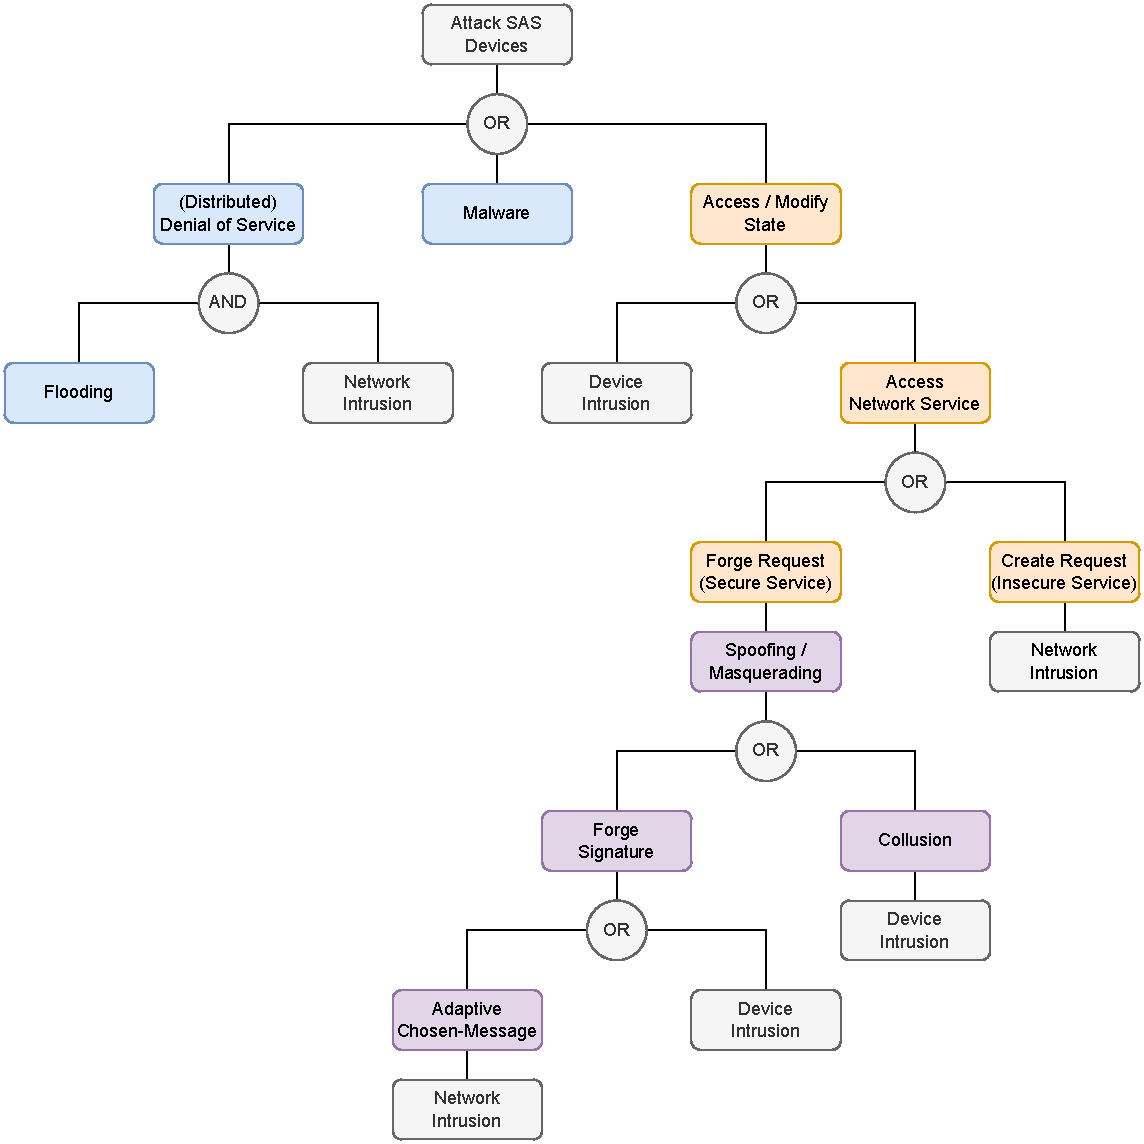
\includegraphics[width=1.0\linewidth]{figures/attack_tree_device.drawio.pdf}
    \caption{Attack tree comprising cyberattacks that endanger the functionality of SAS devices.}
    \label{fig:attack_tree_device}
\end{figure}

\section{Security Policies}
\label{sec:approach:security_policies}
The CASC-SAS approach enforces a set of security policies with the purpose of satisfying the aforementioned requirements and defending a SAS against cyberattacks.
The objective of these policies is not merely to safeguard the equipment of the CASC-SAS approach, but rather to ensure the continuous operation of SAS devices, including IEDs and MUs.
The security policies represent mandatory rules for the operation of a SAS secured by the CASC-SAS approach.
While the attack trees discussed in \autoref{sec:approach:attacks} provide insight into potential adversarial strategies, the proposed security policies represent mitigation strategies for potential cyberattacks.
The cyberattacks that can be mitigated by enforcing the security policies are shown in \autoref{tab:security_policies:attacks}.
The classification of the cyberattacks is based on the classifications illustrated in \autoref{fig:attack_classification}, \autoref{fig:attack_tree_communication}, and \autoref{fig:attack_tree_device}.
Moreover, the security requirements, as introduced in \autoref{sec:approach:requirements}, that can be satisfied by enforcing the security policies are shown in \autoref{tab:security_policies:requirements}.

\begin{description}
    \item[Policy I:] Data Frame Signing and Verification\\%SEC 1/2/3
    The authenticity, integrity, and non-repudiation of exchanged messages on SAS networks are safeguarded by employing cryptographic mechanisms for signing and verification, i.e., digital signatures if PKC is used or MAC if SKC is used.
    This security policy is enforced for each individual data frame of the data link layer to support Ethernet-based SAS protocols such as GOOSE and SV.
    The integration of signing and verification into the OSI protocol stack of two generic Ethernet-based SAS applications within a switched LAN is visualized in \autoref{fig:ethernet_app_protocol_stack}.
    In the shown protocol stack, signing and verification reside within the presentation layer directly below an Ethernet-based application, e.g., a GOOSE or SV application.
    \begin{figure}
        \centering
        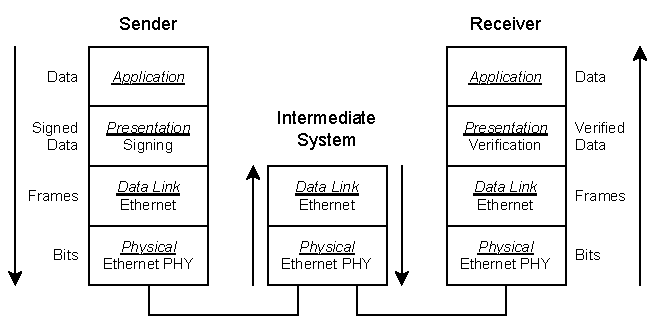
\includegraphics[width=0.7\linewidth]{figures/signed_ethernet_app_protocol_stack.drawio.pdf}
        \caption{Protocol stack of Ethernet-based SAS applications using data verification.}
        \label{fig:ethernet_app_protocol_stack}
    \end{figure}
    %
    \item[Policy II:] Data Frame Access Control\\%SEC 4
    Unauthorized access to service interfaces provided by SAS devices is prevented by employing access control.
    As discussed above, this security policy is enforced for each individual data frame of the data link layer to support Ethernet-based SAS protocols.
    In other words, CASC-SAS checks if a data frame is authorized before delivering it to a SAS application.
    %
    \item[Policy III:] Flow-Based Time-Dependent Authorization\\%SEC 5/6
    Authorization mechanisms are deployed to specify the privileges of communicating entities in a SAS and, thus, enable access control.
    Since a SAS environment is non-static with regard to its state, authorizations have to be time-dependent as well.
    Moreover, authorizations have to be fine-grained and flexible to satisfy the PoLP and SoD security requirements.
    Nevertheless, authorizations have to be network-traffic-flow-based, i.e., applicable to any sequence of data frames with common properties passing through the SAS network, to reduce evaluation overhead and management overhead.
    %
    \item[Policy IV:] Data Frame Sequencing\\%SEC 1, AVA 1/2
    Sequencing of exchanged messages is used to safeguard the system's integrity by mitigating intentional or accidental re-ordering, replaying, and delaying of messages.
    For this purpose, a timestamp is appended to each individual data frame sent.
    A receiver may utilize the timestamp for two distinct purposes.
    Firstly, the receiver interprets the timestamp as sequence number to reject re-ordered and replayed data frames of a network traffic flow.
    Secondly, the receiver may use the timestamp to calculate the average communication latency and its standard deviation to detect infrequent delaying of data frames.
    For the latter case, no time synchronization between sender and receiver is required, as only the deviation from the average is relevant for the classification of delayed data frames.
    %
    \item[Policy V:] Flow-Based Ingress Buffer Management\\%SEC 1, AVA 1/2
    Congestions of exchanged messages in network ingress buffers of SAS devices have to be avoided to mitigate intentional or accidental DoS due to message flooding.
    CASC-SAS employs flow-based buffer management to avoid message congestions.
    The flow-based buffer management limits the number of processed messages of a network traffic flow within a specific time interval.
    If the processing limit is reached, a receiver may either reject received data frames belonging to the network traffic flow or replace buffered data frames with received ones.
\end{description}
\begin{table}
    \centering
    \small
    \caption{Adversarial attacks mitigated by CASC-SAS security policies.}
    \label{tab:security_policies:attacks}
    \begin{tabular}{c c c | c c c c c}
    \toprule
    Adversarial Attack & \multicolumn{2}{c |}{Classification} & \multicolumn{5}{c}{Policy}\\
    & Security Objective & Adversarial Objective & I & II & III & IV & V\\
    \midrule
    % Availability
    Malware            & Availability & Device        &   & X & X &   &   \\
    Flooding           & Availability & Device        &   &   &   &   & X \\
    Time-Delay         & Availability & Communication &   &   &   & X &   \\
    % Integrity
    False Data Injection  & Integrity & Dev. / Comm.  & X & X & X &   &   \\
    Message Forgery       & Integrity & Device        & X &   &   &   &   \\
    Message Modification  & Integrity & Communication & X &   &   &   &   \\
    Message Replay        & Integrity & Communication &   &   &   & X &   \\
    % Authenticity
    Spoofing / Masquerading & Authenticity & Dev. / Comm. & X &   &   &   &   \\
    Adaptive Chosen-Message & Authenticity & Dev. / Comm. & X &   &   &   &   \\
    Collusion               & Authenticity & Dev. / Comm. & X &   &   &   &   \\
    \bottomrule
    \end{tabular}
\end{table}
\begin{table}
    \centering
    \small
    \caption{Security requirements satisfied by CASC-SAS security policies.}
    \label{tab:security_policies:requirements}
    \begin{tabular}{r l | c c c c c}
    \toprule
    \multicolumn{2}{c |}{Requirement} & \multicolumn{5}{c}{Policy}\\
    & & I & II & III & IV & V\\
    \midrule
    RQ.SEC.1: & Payload Integrity & X & & & X\textsuperscript{1} & X\textsuperscript{2} \\
    RQ.SEC.2: & Sender Authenticity & X & & & & \\
    RQ.SEC.3: & Authorship Non-Repudiation & X & & & & \\
    RQ.SEC.4: & Access Control & & X & & & \\
    RQ.SEC.5: & Principle of Least Privilege & & & X & & \\
    RQ.SEC.6: & Separation of Duties & & & X & & \\
    \bottomrule
    \end{tabular}\\
    \footnotesize
    \textsuperscript{1} Prevents re-ordering, replaying, and delaying of valid messages.\\
    \textsuperscript{2} Prevents loss of valid messages due to message flooding.
\end{table}

\section{Security Architecture}
\label{sec:approach:casc:architecture}
In the following, we present the security architecture of the proposed approach.
The CASC-SAS approach is based on a dual-path four-layered architecture.
The four layers of the architecture are presented in \autoref{sec:approach:casc:architecture:layers}.
Moreover, the two paths of the architecture are further discussed in \autoref{sec:approach:casc:architecture:paths}.

\subsection{Four-Layered Architecture}
\label{sec:approach:casc:architecture:layers}
The CASC-SAS architecture is non-strictly layered and consists of four open layers.
The goal of the layered architecture is the separation of different domains and levels of abstraction within the CASC-SAS approach.
An upper layer may use services provided by a lower layer but not vice versa.
Moreover, since the layering is non-strict, an upper layer is not restricted to the services provided by its direct predecessor, but may bypass lower layers.
The four layers of the CASC-SAS architecture and their provided services are defined in the following sections.

\subsubsection{Layer 3: Domain}
The domain layer is the uppermost layer of the architecture.
The domain layer represents the domain-specific applications and the exchange of domain-specific messages.
We assume that the domain layer does not provide means for secure message exchange between entities.
As a consequence, the domain layer relies on the secure message exchange provided by lower layers.
%Provides insecure domain-specific messages to be exchanged between two different SAS devices\dots

\subsubsection{Layer 2: Cybersecurity}
The cybersecurity layer encompasses algorithms and protocols used to satisfy the security requirements.
Additionally, security workflows and mechanisms for the enforcement of security policies are located at this layer.
Consequently, the cybersecurity layer provides secure message exchange services to the domain layer.
The SABAAC concept of CASC-SAS is part of this architectural layer.
SABAAC provides authorization and access control to satisfy the security requirements access control, PoLP, and SoD.
%Provides authorization and access control to satisfy access control, PoLP, and SoD.

\subsubsection{Layer 1: Cryptography}
The cryptography layer provides cryptographic algorithms and schemes to higher layers of the architecture.
The exchange of cryptographic control messages enables cryptographic workflows such as key generation, key distribution, key revocation, and server-aided cryptography.
The CASA core concept of CASC-SAS is located at the cryptography layer.
CASA provides authentication means via digital signatures to higher levels of the architecture.
Accordingly, CASA provides services that satisfy the security requirements integrity, authenticity, and non-repudiation.

\subsubsection{Layer 0: Message Exchange}
The lowermost layer of the CASC-SAS architecture is referred to as message exchange layer.
The message exchange layer provides reliable and unreliable message exchange between devices in a network to higher layers.
The message exchange layer represents an abstraction of the physical layer, data link layer, network layer, and transport layer of a conventional OSI network stack.
%Provides reliable and unreliable message exchange between devices in a network.

\subsubsection{Example: Domain-Specific Communication}
\begin{figure}
    \centering
    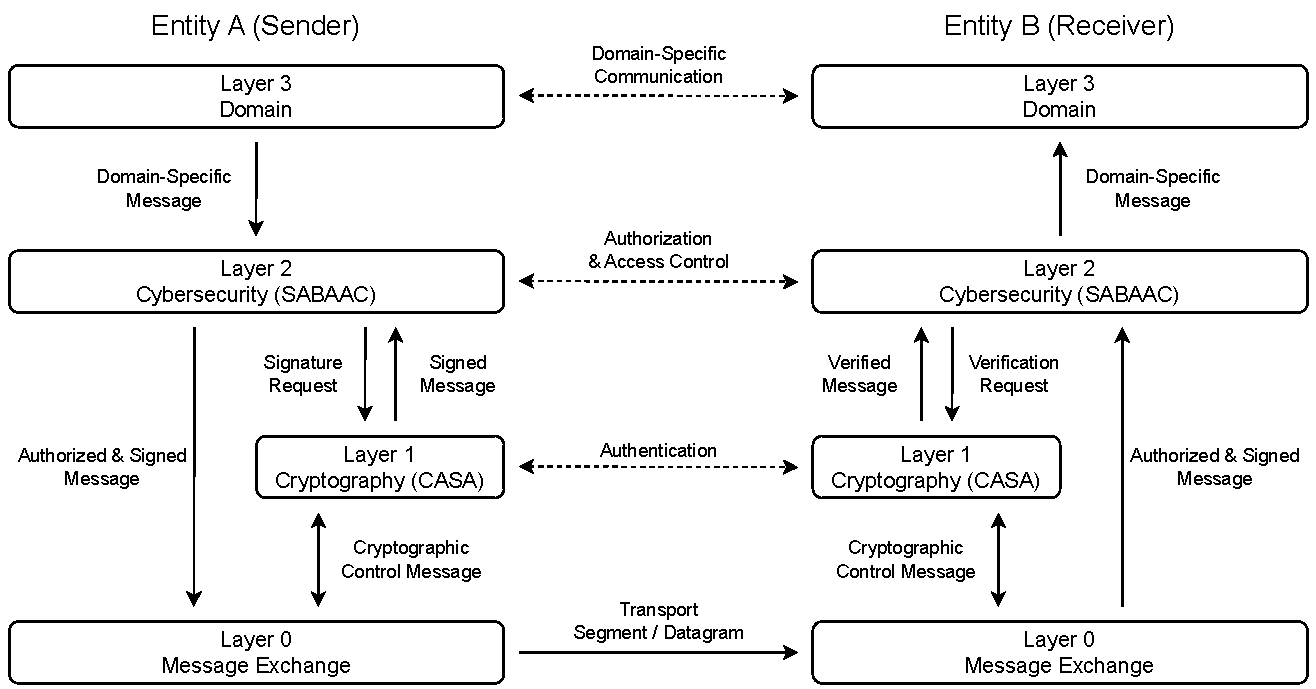
\includegraphics[width=1.0\linewidth]{figures/layers_request_example.drawio.pdf}
    % \caption{An exemplary domain-specific communication between a sending and receiving entity including the involved CASC-SAS layers and messages exchanged between the architectural layers.}
    \caption{Exemplary message exchange in four-layered CASC-SAS architecture.}
    \label{fig:layers_request_example}
\end{figure}
An exemplary domain-specific communication between a sending entity and receiving entity is shown in \autoref{fig:layers_request_example}.
The figure shows the four layers of the CASC-SAS architecture at the sender and receiver.
Moreover, the different messages exchanged between the layers are shown.
While the invocation of services is restricted to predecessor layers, message exchange resulting from an invocation may occur bidirectionally.
The presented domain-specific communication is initiated by entity A.
Therefor, an application at the domain layer of entity A creates a domain-specific message and delivers it to the cybersecurity layer.
The yet unsigned and non-authorized message is then authorized by SABAAC and forwarded to CASA at the cryptography layer for signing.
Subsequently, the signed and authorized message is forwarded to the receiver using the either reliable or unreliable network transport services provided by the message exchange layer.
Upon arrival at the receiver, the message exchange layer delivers the signed and authorized message to the cybersecurity layer.
The messages are then verified by the cybersecurity layer before forwarding them to the domain layer and application.
For the purpose of message verification, the cybersecurity layer enforces the CASC-SAS security policies.
The access control policy is enforced by verifying the message authorization.
Moreover, the message is forwarded to the cryptography layer for digital signature verification.

\subsection{Dual-Path Architecture}
\label{sec:approach:casc:architecture:paths}
%Data Path (Online, time-critical communication, Domain-Specific Messages) \& Control Path (Offline, Non-Time Critical communication, CASC-SAS Messages)\dots
In addition to the separation into different layers, the occurring message exchanges within the CASC-SAS architecture are logically divided into two communication paths.
The two paths are referred to as data path and control path.

The messages on the data path are directly related to the forwarding of domain-specific payload from a sending entity to a receiving entity.
Besides the domain-specific messages, control messages required for the message forwarding are transported on the data path.
This message-related communication includes server-aided signing and verification requests as well as access control.
As a consequence, the data path is used for traffic-intensive and time-critical message exchange.

The messages on the control path are used for the exchange of management information and do not carry payload that is directly related to domain-specific messages.
The components of the CASC-SAS approach use control path messages for layer-internal communication between different devices.
The cryptography layer uses control messages for key generation, distribution, and revocation.
The cybersecurity layer uses control messages for tasks such as policy management.
As a result, the communication occurring on the control path is less traffic-intensive and less time-critical.

\section{Certificateless Attribute-Based Server-Aided Authentication}
\label{sec:approach:casa}
In the following section, we present the \textbf{C}ertificateless \textbf{A}ttribute-Based \textbf{S}erver-Aided \textbf{A}uthentication (CASA) concept.
CASA is a CL-PKC approach.
Consequently, neither certificates nor key escrow are required~\cite{AlRiyami2003}.
The goal of CASA is to provide cryptographic protocols, algorithms, and schemes for key generation, distribution, and revocation as well as signing and verification.
Moreover, the goal of CASA is to enable and support more abstract cybersecurity mechanisms like authorization and access control of the CASC-SAS approach.
Therefore, CASA represents the foundation of the employed CASC-SAS cybersecurity mechanisms.

%Since CASA is a CL-PKC approach, neither certificates nor key escrow is required~\cite{AlRiyami2003}.
%Moreover, the CASA approach proposes a key generation that is not only based on subject identities but rather enables public keys and private keys based on arbitrary attributes of subjects or even groups of subjects.
%The key generation of the CASA approach is inspired by the alternative CL-PKC key generation technique proposed by \citeauthor{AlRiyami2003} \cite{AlRiyami2003}.
%The defining characteristics of the alternative key generation is the derivation of partial private keys from public keys and identities.
%As a consequence, an entity has to generate its public key before it can request a partial private key from the CAPP.
%This alternative key generation enables sending of partial private keys over unsecure channels and reduces the required trust in the CAPP.
%Furthermore, this technique allows only one public key to be created for a specific private key.

\subsection{Administration \& Processing Platform}
The CASA Administration and Processing Platform (CAPP) represents the central component of the CASA approach.
The main objective of the CAPP is the provisioning of services required for the realization of cryptographic protocols.
While CASA also provides its own signature scheme $\mathcal{S}_{CASA}$, which is further discussed in \autoref{sec:casa:scheme}, the CAPP and its protocols are algorithm-agnostic.
The use of an algorithm-agnostic central component in the CASA approach is based on the idea, that different cryptographic algorithms and schemes might be optimal solutions for different problems.
This idea is inspired by the cipher suites and cipher transitioning of the TLS protocol \cite{rfc8446}.
The support of different algorithms and schemes enables devices to choose the cryptographic approach, that fits their security requirements and performance constraints best.

\subsubsection{Server-Aided Cryptography}
As PKC mechanisms may consist of computationally complex algorithms and operations, a core task of the CAPP is to enable and support server-aided PKC.
By supporting server-aided PKC, CASA encourages the utilization of server-aided CL-PKC schemes for time-critical applications.
To make CASA server-aided, the CAPP supports devices by handling computationally expensive algorithms instead of executing them locally on resource-constrained devices.
To minimize the required trust, the CAPP may only handle certain computations, e.g., partially sign or verify a request of a device.
This server-aided approach enables resource-constrained devices to apply secure PKC algorithms and schemes in a time-critical OT environment.

In the following, we employ the concept of server-aided PKC for the verification process.
As stated by \citeauthor{Wu2008} \cite{Wu2008}, a server-aided verification process has to satisfy the property of being computation-saving.
A server-aided verification process $V_{Aided}$ is computation-saving if the computational costs for the verifier are strictly less than the costs of non-server-aided verification $V_{Conventional}$.
In other words, $V_{Aided}$ is computation-saving if the equation $Cost(V_{Aided}) < Cost(V_{Conventional})$ holds.

\subsubsection{Online \& Offline Cryptography}
Since CASA is tailored for time-critical communication, the approach aims to reduce the required time for cryptographic algorithms.
In addition to server-aided cryptography, this time reduction is achieved by precomputation.
For this purpose, each step of an algorithm is classified as either online or offline.
Online steps depend on the sender's public key, the digital signature, or the message.
Consequently, online steps cannot be precomputed.
Nevertheless, specific online steps can be accelerated via server-aided cryptography.
Offline steps depend on information that is available before any message exchange occurs.
Therefore, offline steps can be precomputed either at the CAPP or at client-side to reduce the required time for cryptographic operations.

\subsection{Algorithm-Agnostic Public-Key Exchange Protocol}
The Algorithm-agnostic PKC EXchange (APEX) protocol represents the primary protocol of CASA.
The main objective of the protocol is the exchange of information between the CAPP and other devices within a SAS.
An APEX message exchange is always initiated by sending a request to the CAPP.
Consequently, the protocol can be classified as a request-response client-server protocol.
Furthermore, the protocol is based on a stateless communication pattern that establishes no sessions at the CAPP.
In other words, a message exchange is completed as soon as the APEX reply is sent to the requestor.

The APEX protocol comprises five so-called transactions.
A transaction represents a request-response pair of the protocol.
The transactions of the protocol are defined as follows:
\begin{description}
    \item[Transaction I:] Registration\\
    A device within a SAS sends a registration request to establish its identity and its initial public key at the CAPP.
    For this purpose, the device encapsulates its public key and its identifying attributes in the registration request.
    \item[Transaction II:] Re-Registration\\
    The process of linking a new public key to existing attributes, or modifying an already registered public key is referred to as re-registration. 
    By issuing a re-registration, devices may register multiple public keys, e.g., for different cryptographic algorithms.
    A re-registration request has to be verifiable with one of the registered public keys of a device.
    If the re-registration request cannot be verified, it is rejected by the CAPP.
    \item[Transaction III:] Revocation\\
    The revocation transaction allows devices to revoke a registered public key by removing it from the CAPP.
    The revocation is referred to as deregistration, if it is used to revoke the last registered public key of a device.
    \item[Transaction IV:] Query\\
    The query transaction allows devices to retrieve a specific public key from the CAPP.
    To identify the requested public key, the sender of the request has to encapsulate the identifying attributes of the key owner.
    \item[Transaction V:] Computation\\
    A device may issue a computation request in order to make use of server-aided operations provided by the CAPP.
    Besides the operation-dependent parameters, the request must contain an identification of the requested operation.
\end{description}

\subsection{Signature Scheme $\mathcal{S}_{CASA}$}
\label{sec:casa:scheme}
The CASA signature scheme $\mathcal{S}_{CASA} = (I, G_{PPK}, G_{SK}, S_i, S_{AGG}, V_{SAV}, V_{ENT})$ is a seven-tuple of algorithms.
The algorithms comprise an initialization algorithm $I$, a partial private key generation algorithm $G_{PPK}$, a private key generation algorithm $G_{SK}$, a signing algorithm $S_i$, a signature aggregation algorithm $S_{AGG}$, a partial server verification algorithm $V_{SAV}$, and an entity verification algorithm $V_{ENT}$.
In the following sections, the specific algorithms are further discussed.

%The definition of the CASA signature scheme is based on the definition of digital signature schemes provided by \citeauthor{Boneh2023} \cite{Boneh2023}.
%Moreover, since CASA is a CL-PKC approach, the signature scheme has been adapted from the schemes and concepts presented by \citeauthor{AlRiyami2003} \cite{AlRiyami2003} and \citeauthor{Ramadan2023} \cite{Ramadan2023}.
%The proposed server-aided verification concept and algorithms are inspired by schemes proposed by \citeauthor{Ramadan2020} \cite{Ramadan2020}, \citeauthor{Girault2005} \cite{Girault2005} and \citeauthor{Wu2008} \cite{Wu2008}.

%\subsubsection{Security Model}
%The proposed signature scheme $\mathcal{S}_{CASA}$ is a secure signature scheme if it is existentially unforgeable under an adaptive chosen-message attack (EUF-CMA)~\cite{Boneh2023, Goldwasser1988}.
%To create an existential forgery, i.e., output a valid pair of message and signature for a new message, an adversary carrying out a CMA can request valid signatures from an entity for any message of his choice.
%While non-adaptive CMA restricts the adversary to a fixed set of messages chosen prior to the attack, adaptive CMA allows the adversary to request signatures of messages depending on previously obtained signatures.
% \citeauthor{Goldwasser1988} describe an adaptive CMA as most powerful attack possible for an enemy restricted to using the signature scheme.

\subsubsection{Initialization Algorithm $I$}
The initialization algorithm $(\rho, s) \leftarrow I(\lambda)$ takes the security parameter $\lambda$ as input and outputs the public system parameters $\rho$ and the master secret $s$.
The initialization algorithm is executed by the CAPP.
After the execution, $\rho$ is publicly available to all entities, whereas $s$ is only known to the CAPP.
The initialization algorithm consists of the following steps:
\begin{enumerate}
    \item Define the bilinear groups $G_1$, $G_2$, and $G_T$ of prime order $q$, generators $g_1 \in G_1$ and $g_2 \in G_2$, and a bilinear pairing $e$:
    \[
        e: G_1 \times G_2 \rightarrow G_T
    \]
    A map $e$ is a bilinear pairing if it fulfills the following properties:
    \begin{enumerate}
        \item Bilinearity: $e(P^a, Q^b) = e(P, Q)^{ab}$ for all $P \in G_1, Q \in G_2$ and $a, b \in \mathbb{Z}_q^*$.
        \item Non-Degeneracy: $e(P, Q) \neq 1$ for $P \in G_1, Q \in G_2$
        \item Computability: There is an efficient algorithm to compute $e(P, Q)$ for any $P \in G_1, Q \in G_2$
    \end{enumerate}
    \item Define the cryptographic hash functions $H_1$, $H_2$, and $H_3$:
    \[
        H_1: \{0,1\}^* \to G_1,
        \quad H_2: \{0,1\}^* \to \mathbb{Z}_q^*,
        \quad H_3: \mathbb{Z}_q^* \to G_2.
    \]
    \item Generate the master secret $s$ and compute the master public key $pk_m$:
    \[
        s \in \mathbb{Z}_q^*,
        \quad pk_m = g_2^{s}.
    \]
    \item Publish the public system parameters $\rho$:
    \[
        \rho = (G_1, G_2, G_T, q, e, g_1, g_2, pk_m, H_{1}, H_{2}, H_{3}).
    \]
\end{enumerate}

\subsubsection{Partial Private Key Generation Algorithm $G_{PPK}$}
The partial private key generation algorithm $ppk_i \leftarrow G_{PPK}(\rho, s, ID_i, ATT_i)$ takes the public system parameters $\rho$, the master secret of the CAPP $s$, the identifier $ID_i$ of entity $A_i$, and the attributes $ATT_i$ of entity $A_i$ as input.
The algorithm outputs the partial private key $ppk_i$ of entity $A_i$.
The partial private key generation is executed by the CAPP on request of entity $A_i$.
After the execution, the CAPP provides the partial private key to the corresponding entity.
The partial private key generation algorithm consists of the following steps:
\begin{enumerate}
    \item Compute the partial private key $ppk_i$ on request of entity $A_i$:
    \[
        ppk_i = H_1(ID_i || ATT_i)^{s}.
    \]
    \item Provide the partial private key $ppk_i$ to entity $A_i$.
\end{enumerate}

\subsubsection{Private Key Generation Algorithm $G_{SK}$}
The private key generation algorithm $sk_i \leftarrow G_{SK}(\rho, ppk_i)$ takes the public system parameters $\rho$, and the partial private key $ppk_i$ of entity $A_i$ as input.
The algorithm outputs the private signing key $sk_i$ of entity $A_i$.
The private key generation algorithm consists of the following steps:
\begin{enumerate}
    \item Generate a random secret value $\chi_i$:
    \[
        \chi_i \in \mathbb{Z}_q^*.
    \]
    \item Set the private signing key $sk_i$:
    \[
        sk_i = (ppk_i, \chi_i).
    \]
\end{enumerate}

\subsubsection{Signing Algorithm $S_i$}
The signing algorithm $\sigma_{i} \leftarrow S_i(\rho, sk_i, m, T)$ takes the public system parameters $\rho$, the private signing key $sk_i$ of entity $A_i$, a message $m$, and an access policy $T$ as input, and outputs the signature $\sigma_{i}$.
In other words, the signing algorithm $S_i$ is used by the sender $A_i$ of a message $m$ to generate a digital signature $\sigma_{i}$.
The generated digital signature $\sigma_{i}$ is associated with the message $m$, the sender's private signing key $sk_i$, and an access policy $T$.
The signing algorithm consists of the following steps:
\begin{enumerate}
    \item Check if the attributes $ATT_i$ of entity $A_i$ satisfy the policy $T$, and abort the process otherwise.
    \item Compute the hash $h$ of the message $m$:
    \[
        h = H_2(m || T).
    \]
    \item Compute the signature $\sigma_i$ using the private signing key $sk_i$:
    \[
        \sigma_i = ppk_i \cdot H_3(h)^{\chi_i}.
    \]
\end{enumerate}

\subsubsection{Signature Aggregation Algorithm $S_{AGG}$}
The signature aggregation algorithm $\sigma_{agg} \leftarrow S_{AGG}(\sigma_{1 \dots n})$ takes $n$ signatures $\{\sigma_i | 1 \leq i \leq n\}$ as input.
The algorithm outputs an aggregated signature $\sigma_{agg}$:
\[
    \sigma_{agg} = \prod_{i=1}^n \sigma_i.
\]

\subsubsection{Partial Server Verification Algorithm $V_{SAV}$}
The partial server verification algorithm $P_{CAPP} \leftarrow V_{SAV}(\rho, s, \sigma_{agg}, ID_{1 \dots n}, ATT_{1 \dots n})$ takes the public system parameters $\rho$, the master secret of the CAPP $s$, an aggregated signature $\sigma_{agg}$, the entity identifiers $\{ID_i | 1 \leq i \leq n\}$, and the entity attributes $\{ATT_i | 1 \leq i \leq n\}$ as input.
The algorithm outputs the partial verification $P_{CAPP}$.
The partial server verification algorithm consists of the following steps:
\begin{enumerate}
    \item Compute the aggregated public key $pk_{agg}$:
    \[
        pk_{agg} = \prod_{i=1}^n H_1(ID_i || ATT_i)^{s}.
    \]
    \item Compute the partial verification $P_{CAPP}$:
    \[
        P_{CAPP} = e(pk_{agg} \cdot \frac{\sigma_{agg}}{pk_{agg}}, g_2).
    \]
\end{enumerate}

\subsubsection{Entity Verification Algorithm $V_{ENT}$}
The entity verification algorithm $\delta \in \{accept, reject\} \leftarrow V_{ENT}(\rho, \sigma_{agg}, P_{CAPP})$ represents the final step of the verification process.
The algorithm takes the public system parameters $\rho$, the aggregated signature $\sigma_{agg}$, and the partial verification $P_{CAPP}$ as input.
The algorithm outputs the verification decision $\delta$ which is either $accept$ or $reject$.
In other words, the verification algorithm $V_{ENT}$ is used by a message receiver to verify a message $m$ sent by entity $A_i$ based on an appended signature $\sigma_{agg}$.
As $\sigma_{agg}$ is associated with the message $m$ and the sender's private signing key $sk_i$, it allows the receiver to verify the integrity and authenticity of the received message $m$.
The entity verification algorithm consists of the following steps:
\begin{enumerate}
    \item Compute the bilinear pairing $P_{Entity}$:
    \[
        P_{Entity} = e(\sigma_{agg}, g_2).
    \]
    \item Accept $m$ if the following equation holds and reject otherwise:
    \[
        P_{Entity} \overset{!}{=} P_{CAPP}
    \]
\end{enumerate}

\section{Server-Aided Attribute-Based Authorization \& Access Control}
\label{sec:approach:sabaac}
The second core concept of the CASC-SAS approach is the \textbf{S}erver-Aided \textbf{A}ttribute-\textbf{B}ased \textbf{A}uthorization and \textbf{A}ccess \textbf{C}ontrol (SABAAC).
The SABAAC approach enables the employment of attribute-based authorization and access control for time-critical SAS communication.
Therefore, the approach prevents unauthorized access and extraction of information.
The approach enables CASC-SAS to satisfy the access control, PoLP, and SoD security requirements.
Moreover, the expressive and flexible yet computationally expensive ABAC policies are handled in a server-aided manner to satisfy the strict time constraints of the SAS domain.

Our authorization and access control approach represents a security concept that is located on the cybersecurity layer of the CASC-SAS architecture.
Thus, it relies on secure authentication services provided by CASA.
As a consequence, the approach assumes that efficient and secure signing and verification algorithms are available.
In other words, CASA provides secure cryptographic algorithms and schemes that enable SABAAC to realize secure authorization and access control.

The proposed authorization and access control approach is based on a function-oriented component-based architecture.
The architecture and components are further discussed in \autoref{sec:approach:sabaac:architecture}.
Furthermore, the approach is divided into two central tasks.
The first task is referred to as delegated attribute-based authorization.
The delegated attribute-based authorization is responsible for the access control policy creation, management, storage, and distribution.
This task partially takes place prior to access requests and corresponding access decisions.
The delegated attribute-based authorization protocol is further discussed in \autoref{sec:approach:sabaac:authorization}.
The second central task is referred to as delegated ABAC.
The delegated ABAC is responsible for the policy decision exchange and policy enforcement.
This task takes place when an entity initiates the communication with another entity.
The delegated ABAC protocol is further discussed in \autoref{sec:approach:sabaac:accesscontrol}.
An overview of the SABAAC architecture, components, and protocols is shown in \autoref{fig:sabaac_protocols_overview}.
\begin{figure}
    \centering
    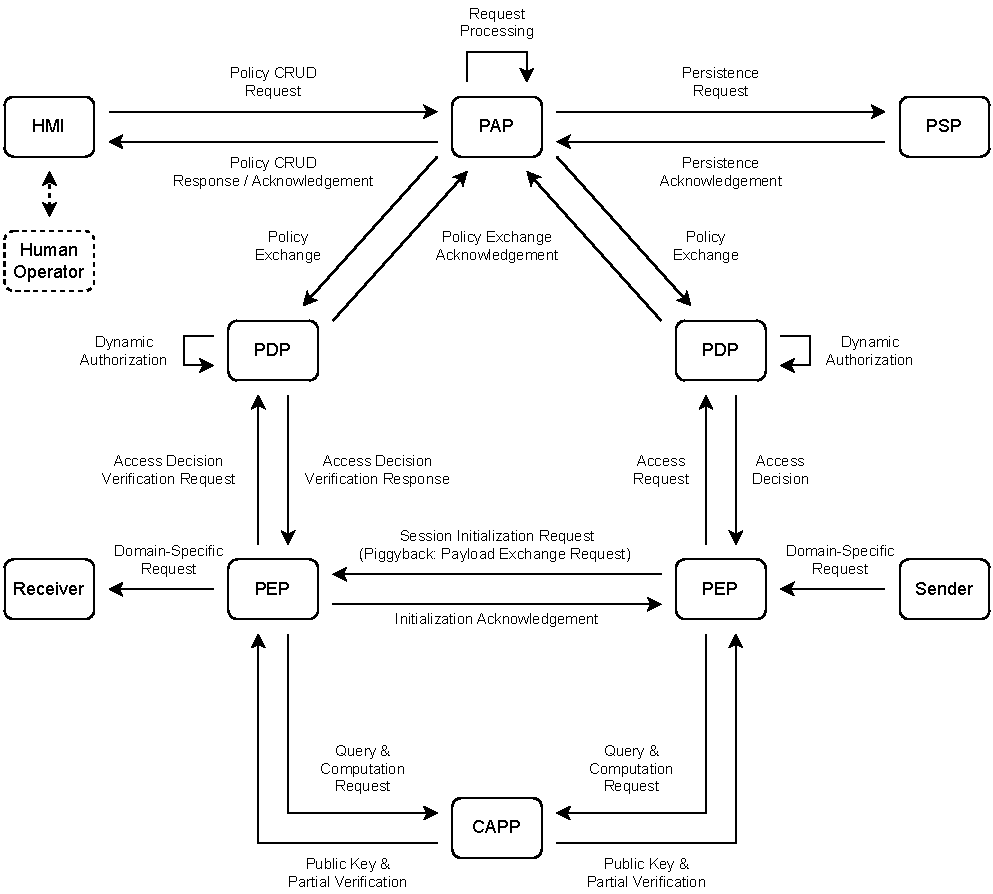
\includegraphics[width=1.0\linewidth]{figures/SABAAC_protocols_overview.drawio.pdf}
    % \caption{Component-based architecture and communication protocols of the SABAAC approach, including the four SABAAC components, their interrelationships, and the integration of CASA components and services into the authorization and access control workflow.}
    \caption{Function-oriented component-based architecture of the SABAAC approach.}
    \label{fig:sabaac_protocols_overview}
\end{figure}

\subsection{Authorization \& Access Control Architecture}
\label{sec:approach:sabaac:architecture}
The component-based architecture of our authorization and access control approach consists of four functional units.
These functional units have been adapted from the access control mechanism functional points presented by \citeauthor{Hu2014} \cite{Hu2014}.
Each functional unit is represented by a component that offers a set of services.
The components of the architecture are TTPs since the semantic validity of their provided services is not verifiable by the service consumers.
%We specify the components as semi-trusted for the access control problem due to the restriction to access control tasks and available mitigation approaches such as multiple instances of a single component.
Strategies to reduce the required trust in specific components, including the deployment of multiple instances of a single component, are discussed in the following sections.
The four components of the architecture are defined below:
\begin{description}
    \item[Policy Administration Point (PAP)] The PAP offers services for the policy creation, management, and distribution.
    The PAP is a component of the delegated attribute-based authorization process and executes the corresponding authorization protocols.
    Moreover, it provides interfaces for policy management services to human operators.
    The PAP accesses the PSP to persist policies and policy changes.
    \item[Policy Storage Point (PSP)] The PSP acts as a repository to make created policies and changes to policies persistent.
    For this purpose, the PSP offers Create, Read, Update, and Delete (CRUD) services to PAP instances.
    The physical PSP instance may be integrated with the PAP component to avoid network communication overhead.
    \item[Policy Decision Point (PDP)] The PDP takes access control decisions by evaluating policies.
    The PDP takes decision on request of a PEP and provides the access control decision to the requesting PEP.
    As a consequence, the PDP is part of the delegated ABAC task of SABAAC.
    Furthermore, in the SABAAC architecture the PDP incorporates the services provided by the context handler, which was introduced by \citeauthor{Hu2014} \cite{Hu2014}.
    Therefore, the PDP not only takes access control decisions on request but is responsible for the policy and attribute evaluation workflow.
    This workflow includes the retrieval of required attributes and speedup techniques such as access decision caching and policy evaluation precomputation.
    \item[Policy Enforcement Point (PEP)] The PEP enforces access control decisions by controlling access to protected objects.
    As a consequence, the PEP is part of the delegated ABAC task of SABAAC.
    The services provided by the PEP rely on access control decisions taken by the PDP.
    % To reduce the required trust in the PDP decision, the PEP can query multiple PDPs to validate the access control decision taken.
    Moreover, in the SABAAC architecture the PEP incorporates the services provided by the Policy Information Point (PIP), which was introduced by \citeauthor{Hu2014} \cite{Hu2014}.
    Accordingly, the SABAAC PEP provides attributes related to its protected objects to the PDP.
\end{description}

\subsection{Access Control Policy}
\label{sec:approach:sabaac:policy}
According to \citeauthor{Hu2014} \cite{Hu2014}, ABAC is an access control model that enables access decisions based on attributes associated with subjects, objects, actions, and the environment of a system.
An ABAC policy represents a set of rules that describe under which environmental conditions a certain subject is granted to perform certain actions on a specific protected object.
The SABAAC approach relies on the concept of attribute-based policies and access control due to the following benefit:
ABAC enables multifactor policy expression, while RBAC and IBAC limit the policy expressiveness by only relying on either roles or identities.
Consequently, the multifactor policy expression enables fine-grained and flexible access control.

\subsubsection{Policy Specification}
The SABAAC approach features a novel strategy for the representation and specification of access control policies.
In this section we introduce the structure of the policies and define the different types of attributes that are supported.
% Moreover, we introduce the SABAAC Policy Specification Language (SPSL) that is used by human operators to specify access control policies.
As defined by the second and third security policy of CASC-SAS in \autoref{sec:approach:security_policies}, the policies are enforced for data frame flows, i.e., sets of data frames with common properties passing through the SAS network.
Accordingly, the objective of an access control policy is twofold.
On the one hand, a policy has to contain information that specifies if the policy is applicable to a certain data frame flow.
On the other hand, a policy must specify which actions should be taken for a matching data frame flow.

\paragraph{Access Control Policy:} $\rho = (action_{\rho}, flow_{\rho}, auxiliary_{\rho})$.\\
A SABAAC policy $\rho$ is represented by a three-tuple, which contains the $action$ to be taken, the $flow$-specifying pattern, and a set of $auxiliary$ attributes specifying additional non-flow-related system characteristics.

\paragraph{Action:} $action \in \{GRANT, DENY\}$.\\
The action of a policy specifies whether a matching data frame flow should be granted or denied.
A data frame from a granted flow may be delivered to a SAS device, whereas a data frame from a denied flow is dropped by a PEP.
The default action of SABAAC is $DENY$ which leads to dropping of all data frames of non-explicitly granted flows.

\paragraph{Flow Pattern:} $flow = \{p_1, \dots, p_n\}$, $p_i(frame) \in \{TRUE, FALSE\}$.\\
The flow pattern of a policy specifies whether the policy is applicable to a specific data frame or not.
For this purpose, the flow pattern consists of a set of frame predicates $p_1, \dots, p_n$.
A frame predicate $p_i$ is a function that assigns a boolean value to an arbitrary data frame.
A predicate $p_i$ matches a frame $f$, if $p_i(f) = TRUE$.
A policy is applicable to a specific data frame if all frame predicates match the frame.
In other words, a policy $\rho = (action_{\rho}, flow_{\rho}, auxiliary_{\rho})$ is applicable to a frame $f$ if the following equation holds:
\[
    \forall p_i \in flow_{\rho}: p_i(f) = TRUE
\]

\paragraph{Auxiliary Attributes:} $auxiliary = \{a_1, \dots, a_n\}$, $a_i(system) \in \{TRUE, FALSE\}$.\\
The auxiliary attributes of a policy specify non-flow-related system attributes that have to be taken into account in order to apply an access control policy.
The auxiliary attributes are specified in the form of so-called system predicates $a_1, \dots, a_n$.
A system predicate $a_i$ is a function that assigns a boolean value to the current system state.
A policy $\rho = (action_{\rho}, flow_{\rho}, auxiliary_{\rho})$ is applicable in a system $s$ if all system predicates match the current system state, i.e., a policy is applicable if the following equation holds:
\[
    \forall a_i \in auxiliary_{\rho}: a_i(s) = TRUE
\]

\subsubsection{Policy Classification}
The utilization of ABAC can avoid explicit authorizations prior to a request \cite{Hu2014}.
In other words, an ABAC policy can be dynamically evaluated at the time of a request.
This dynamic evaluation allows the use of attributes from a time-variable environment.
As stated by \citeauthor{Burmester2013} \cite{Burmester2013}, a real-time attribute represents an attribute whose value is time-dependent.
Given an attribute evaluation function $E_{ATT}$ and a point of time $t$, the value $\lambda_a$ of a real-time attribute $a$ is defined by $E_{ATT}(a, t) = \lambda_a$.

Each SABAAC policy $\rho$ is related to a set of attributes $ATT_{\rho} = ATT_{flow_{\rho}} \cup ATT_{auxiliary_{\rho}}$.
The flow attributes $ATT_{flow_{\rho}}$ consist of all frame-related attributes required for the evaluation of the frame predicates $p_1, \dots, p_n$.
The auxiliary attributes $ATT_{auxiliary_{\rho}}$ consist of all non-flow-related system attributes required for the evaluation of the system predicates $a_1, \dots, a_n$.
To handle policies based on their degree of time-variability, the SABAAC approach classifies policies as follows:
\begin{description}
    \item[Dynamic Policy] A dynamic policy $\rho$ is an ABAC policy whose evaluation relies on at least one time-variable subject, object, environment, or action attribute.
    A policy $\rho$ is dynamic iff $\exists a \in ATT_{\rho}: \exists t_i \neq t_j: E_{ATT}(a,t_i) \neq E_{ATT}(a,t_j)$.
    Due to the time-variable evaluation of dynamic policies, access decisions must have a limited time of validity that corresponds to the change rate of the underlying attribute values.
    As a result, caching of access decisions that are based on dynamic policies should be avoided.
    A dynamic policy is also referred to as real-time policy.
    \item[Static Policy] A static policy $\rho$ is an ABAC policy whose evaluation does not rely on time-variable subject, object, environment, or action attributes.
    A policy $\rho$ is static iff $\forall a \in ATT_{\rho}: \forall t_i,t_j: E_{ATT}(a,t_i) = E_{ATT}(a,t_j)$.
    Since static policies do not rely on time-variable attributes, access decisions can be cached.
    Moreover, due to the non-frequent attribute retrieval and evaluation as well as access decision caching, static policies are a viable solution for low latency message exchange.
    A static policy is also referred to as non-real-time policy.
\end{description}

\subsubsection{Policy Evaluation}
The policy evaluation is the process of deriving an access control decision from an access control policy and enforcing the decision in the SAS.
While the access control policy may depend upon the current system state, the corresponding access control decision is static during a specified period of validity.
As a consequence, the process of evaluating a SABAAC policy can be divided into two related processes:
The PDP-driven dynamic authorization derives an access control decision from an access control policy for the current system state.
The PEP-driven decision enforcement utilizes the result of the dynamic authorization to enforce the SAS policies in a timely manner.

\paragraph{Access Control Decision:} $decision_{\rho} = \{flow_\rho, action_\rho, nexthop, validity\}$.\\
An access control decision or access decision consists of a $flow$-specifying pattern, an $action$ to be taken, a $nexthop$ set specifying the PEPs a matching data frame should be forwarded to, and a period of $validity$.
Accordingly, an access decision is valid for a specific data frame flow in a specific system during a specified period of time.

\paragraph{Dynamic Authorization:} $E_{POL}: Policy \times System \rightarrow Decision$.\\
In the SABAAC approach, the policy evaluation is server-aided and takes partially place at the PDP.
To derive an access decision from an access control policy at the PDP, the dynamic authorization function is used.
The dynamic authorization function of SABAAC is defined as follows:
\[
    E_{POL}(\rho, s_t) =
    \begin{cases}
        (flow_\rho, action_\rho, nexthop, validity) & \text{, if } \forall a_i \in auxiliary_{\rho}: a_i(s) = TRUE,\\
        (flow_\rho, DENY, \emptyset, validity) & \text{, otherwise.}
    \end{cases}
\]
Thus, if the system predicates $a_1, \dots, a_n$ of the policy match the current system state $s_t$, the policy is applicable to data frame flows in the system $s$.
To evaluate the system predicates, the PDP fetches the auxiliary attributes $ATT_{auxiliary_{\rho}} \subseteq s_t$ prior to the evaluation of $a_1, \dots, a_n$.
The validity of the resulting access decision at the point of time $t$ equals the minimal validity of the attribute values in $\{\lambda_k = E_{ATT}(k, t) | k \in ATT_{auxiliary_{\rho}} \subseteq s_t\}$.
Consequently, the validity of an access decision of a dynamic policy is determined by the attribute value that expires first.
The validity of an access decision of a static policy may be limited by specifying a non-attribute-related maximum time of validity, to avoid the utilization of invalid or outdated access decisions.

\paragraph{Decision Enforcement:} $E_{DEC}: Decision \times Frame \rightarrow (Action, Nexthop)$.\\
A PEP uses an access control decision $d_{\rho}$ taken by a PDP to enforce a policy $\rho$ in the SAS.
For this purpose, each data frame $f$ traversing a PEP is matched using $flow_\rho$ to identify the corresponding access decision.
The process of enforcing a policy based on a priorly taken access decision is referred to as decision enforcement.
At the PEPs the decision enforcement for a decision $d_{\rho} = \{flow_\rho, action_\rho, nexthop, validity\}$ and a frame $f$ is performed using the decision enforcement function $E_{DEC}$:
\[
    E_{DEC}(d_{\rho}, f) =
    \begin{cases}
        (action_\rho, nexthop) & \text{, if } \forall p_i \in flow_{\rho}: p_i(f) = TRUE\\
        & \quad \land validity.contains(time.now),\\
        (DENY, \emptyset) & \text{, otherwise.}
    \end{cases}
\]
Thus, if the flow predicates match a data frame, and the decision is still valid, the decision enforcement function returns the action to be taken and the PEPs the frame has to be forwarded to.
Two cases have to be distinguished, if $E_{DEC}(d_{\rho}, f) = (action_\rho, nexthop)$:
\begin{itemize}
    \item \textbf{Outgoing Data Frame:} An outgoing data frame $f$ is forwarded to each $PEP \in nexthop$, if $action_\rho = GRANT$.
    \item \textbf{Incoming Data Frame:} An incoming data frame $f$ is accepted by a receiving $PEP$, if $action_\rho = GRANT$ and $PEP \in nexthop$.
\end{itemize}
If multiple decisions match a data frame $f$ identified by flow attributes $ATT_{f}$, a PEP may choose the decision corresponding to the most specifically matching flow predicates.
When two flow patterns $flow_\gamma$ and $flow_\delta$ of the access control policies $\gamma$ and $\delta$ match a data frame $f \supseteq ATT_{f}$, $flow_\gamma$ is said to match $f$ more specifically than $flow_\delta$ if $ATT_{f} \supseteq ATT_{flow_{\gamma}} \supsetneq ATT_{flow_{\delta}}$.
In case of $(ATT_{flow_{\gamma}} \not \supseteq ATT_{flow_{\delta}}) \land (ATT_{flow_{\gamma}} \not \subseteq ATT_{flow_{\delta}})$, the matching flow patterns and their corresponding access control policies and decisions are said to be conflicting.
A PEP may use a so-called composite decision $d_C$ to resolve two or more conflicting access control decisions $d_1, \dots, d_n$:
\[
    d_C =
    \begin{cases}
        (\bigcup_{i=1}^{n}flow_i, GRANT, \bigcup_{i=1}^{n}nexthop_i, \min_{i=1}^{n}validity_i) & \text{, if } \forall d_i \in \{d_1, \dots, d_n\}:\\
        & \quad action_i = GRANT,\\
        (\bigcup_{i=1}^{n}flow_i, DENY, \emptyset, \min_{i=1}^{n}validity_i) & \text{, otherwise.}
    \end{cases}
\]

\paragraph{Evaluation Strategies:} A Priori, A Posteriori, \& Predicted Evaluation\\
To speed up the policy evaluation and increase the data frame throughput, PEP and PDP instances may rely upon different policy evaluation strategies.
The SABAAC approach distinguishes between three evaluation strategies shown in \autoref{fig:policy_evaluation_strategies} and defined below:
\begin{itemize}
    \item \textbf{A Priori:} The a priori or precomputed evaluation aims to maximize the policy evaluation speed.
    A finite-state machine representing the a priori evaluation strategy at a PDP and PEP is shown in \autoref{fig:apriori_policy_evaluation_strategy}.
    At the PDP, the strategy is applied via precomputation of the dynamic authorization function $E_{POL}$ for all available access control policies of the SAS.
    Accordingly, a PDP refreshes and caches each access decision periodically, and provides it to PEPs if requested.
    At the PEP, a priori evaluation can be achieved by requesting access decisions before data frames are matched and forwarded, i.e., before $E_{DEC}$ is evaluated.
    For this purpose, a PEP requests all relevant access decisions at startup and re-request them from a PDP before the period of validity ends.
    The precomputation strategy results in an increased policy evaluation speed, increased data frame throughput, and decreased network jitter sensitivity.
    The a priori strategy is particularly suitable for periodic message exchanges, such as messages exchanges of the SV protocol.
    However, precomputation and caching of access decisions leads to increased memory utilization.
    Furthermore, periodic refreshing of unused or rarely used access decisions results in non-optimal power efficiency.
    
    \item \textbf{A Posteriori:} The a posteriori or ad-hoc evaluation aims to minimize the memory utilization.
    A finite-state machine representing the a posteriori evaluation strategy at a PDP and PEP is shown in \autoref{fig:aposteriori_policy_evaluation_strategy}.
    In contrast to the a priori strategy, neither the PDP-driven dynamic authorization nor the PEP-driven access decision requests are precomputed or cached.
    As a consequence, for each traversing data frame a PEP requests an access decision from a PDP.
    The PDP evaluates $E_{POL}$ on request and provides the result to the PEP.
    As no access decisions are cached at the PDP and PEP, the a posteriori strategy minimizes the memory utilization.
    The strategy is particularly suitable for non-recurring and non-periodic message exchanges without message fragmentation.
    However, for periodic message exchanges and frequently matching flow patterns the strategy results in non-optimal power efficiency and decreased data frame throughput, as access policies are repeatedly evaluated even if the corresponding access decisions are still valid.

    \item \textbf{Predicted:} The predicted, conditional, or hybrid evaluation aims to optimize data frame throughput, memory utilization, and power efficiency.
    A finite-state machine representing the predicted evaluation strategy at a PDP and PEP is shown in \autoref{fig:predicted_policy_evaluation_strategy}.
    This strategy is inspired by the branch prediction used in microprocessor architectures.
    Instead of relying exclusively upon a priori or a posteriori evaluation, the hybrid evaluation uses a predictor to decide whether an access decision should be refreshed and cached.
    By predicting whether an access decision is required in the next prediction period, PDPs and PEPs are able to avoid unnecessary computation, requesting, and caching of non-required access decisions.
    As for branch predictors in microprocessor architectures, the primary objective of an access decision predictor is the avoidance of cache misses, while optimizing the memory utilization and power efficiency. 
\end{itemize}
\begin{figure}
    \centering
    \begin{subfigure}[t]{0.40\linewidth}
        \centering
        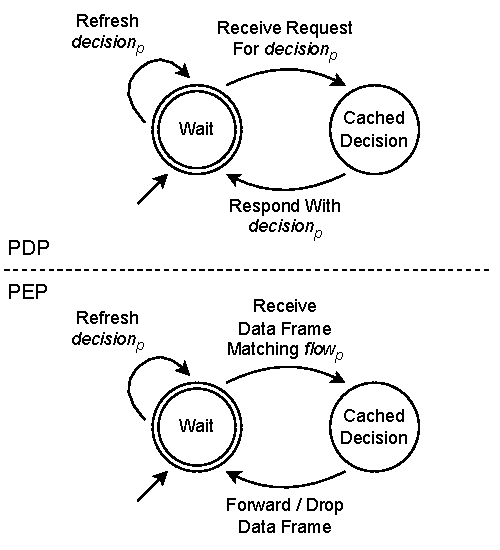
\includegraphics[width=\linewidth]{figures/apriori_evaluation_strategy.drawio.pdf}
        \caption{A priori policy evaluation.}
        \label{fig:apriori_policy_evaluation_strategy}
    \end{subfigure}
    \hfill
    \begin{subfigure}[t]{0.55\linewidth}
        \centering
        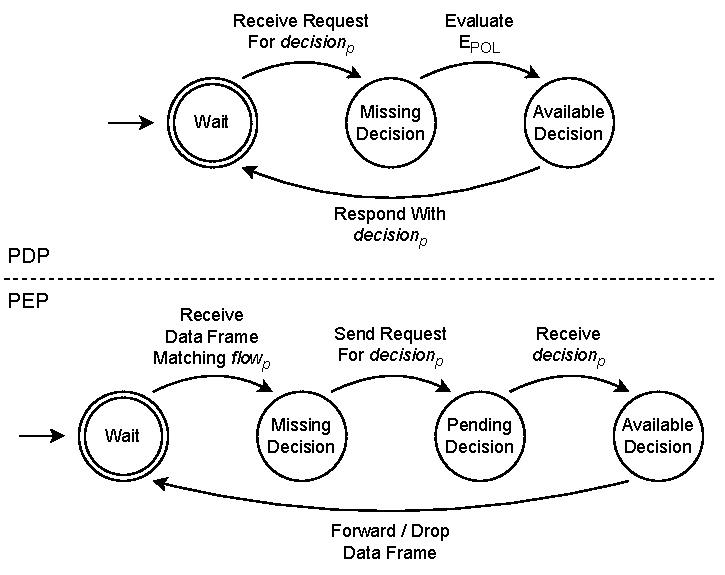
\includegraphics[width=\linewidth]{figures/aposteriori_evaluation_strategy.drawio.pdf}
        \caption{A posteriori policy evaluation.}
        \label{fig:aposteriori_policy_evaluation_strategy}
        \vspace{1.0\baselineskip}
    \end{subfigure}
    \begin{subfigure}[t]{1.\linewidth}
        \centering
        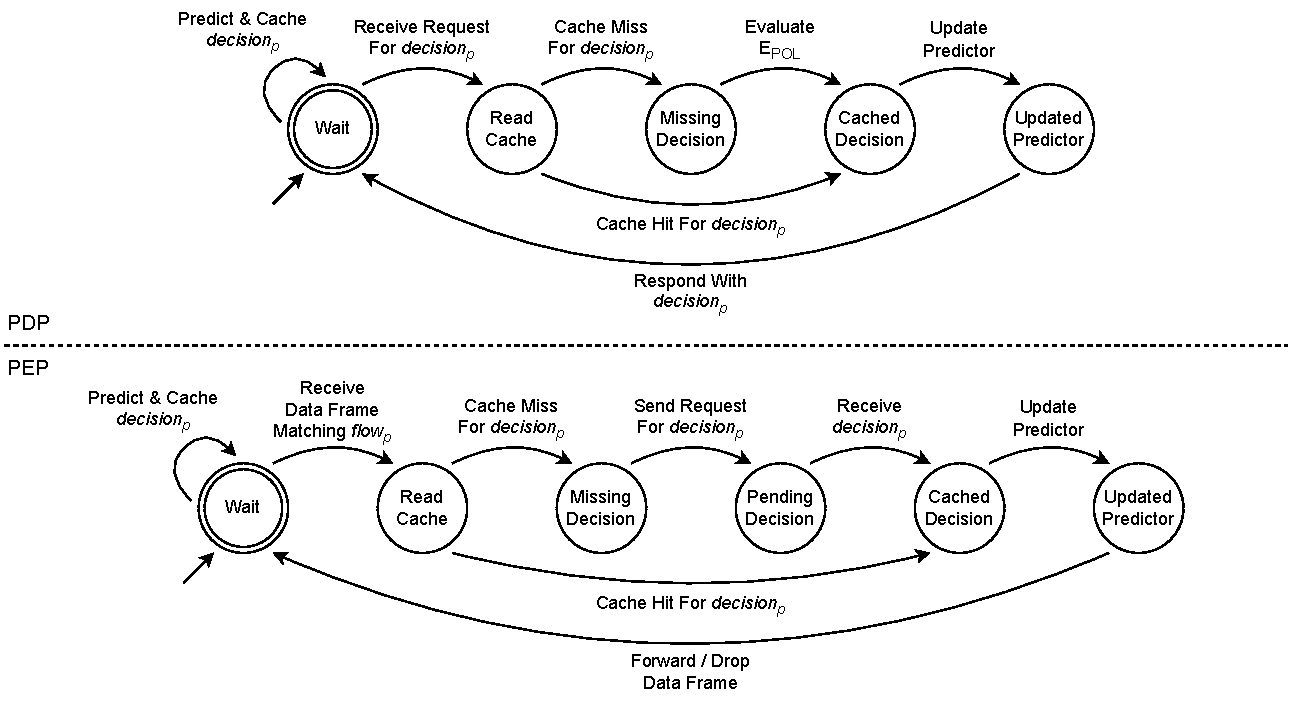
\includegraphics[width=\linewidth]{figures/predicted_evaluation_strategy.drawio.pdf}
        \caption{Predicted policy evaluation.}
        \label{fig:predicted_policy_evaluation_strategy}
    \end{subfigure}
    \caption{Finite-state machines of the SABAAC policy evaluation strategies at the PDP and PEP.}
    \label{fig:policy_evaluation_strategies}
\end{figure}

\subsection{Delegated Attribute-Based Authorization Protocol}
\label{sec:approach:sabaac:authorization}
In the following, we discuss the delegated attribute-based authorization protocol of the SABAAC approach.
Authorization is the process of assigning access privileges for protected objects to subjects \cite{Eckert2023}.
A subject is said to be authorized for a specific request if it has the required access privileges for the request.
We propose an authorization protocol that is responsible for the policy creation, modification, storage, and distribution.
For this purpose, the authorization protocol provides policy management services at the PAP.
Moreover, the authorization protocol provides services for the exchange of policies between the PAP, PSP, and PDP.
The authorization protocol is part of the control path of CASC-SAS, as neither policy management nor policy exchange are directly related to domain-specific messages.

The delegated attribute-based authorization protocol offers reliable services to entities involved in the policy management process, including human operators or intrusion detection and prevention systems. 
It uses signing and verification services provided by CASA to safeguard the integrity and authenticity of messages.
The exchanged messages of the protocol are sequenced, as defined by security policy IV in \autoref{sec:approach:security_policies}, to protect the protocol against intentional or accidental re-ordering, replaying, and delaying of messages.
To guarantee the delivery of messages, the protocol relies on an Automatic Repeat Query (ARQ) approach.
Accordingly, positive acknowledgements and timeout-based retransmissions are used to achieve reliable message transmission over an unreliable communication channel.

As discussed in \autoref{sec:approach:sabaac:policy}, access control policies are classified as either static or dynamic.
Consequently, the authorization protocol has to take the time-variability of access control policies into account.
For this purpose, the authorization protocol consists of three parts or sub-protocols:
\begin{description}
    \item[Static Authorization] The static authorization process is responsible for handling CRUD requests for access control policies.
    The process, the involved components, and the occurring message exchanges are visualized in \autoref{fig:sabaac_authorization_static}.
    The static authorization is initiated by a human operator or an external system responsible for the management of policies.
    When a policy CRUD request arrives at a PAP, it is processed by the PAP according to the requested action.
    In case of a read request, the PAP fetches the requested access control policy from its PSP and returns it to the requestor.
    Create, update, and delete requests are processed by computing a set of changes to be made to the persistent set of access control policies.
    These changes are sent to the PSP via persistence requests.
    As soon as all changes are made to the access control policies, the PSP sends a persistence acknowledgement to the PAP and the PAP acknowledges the initial policy CRUD request.
    \begin{figure}
        \centering
        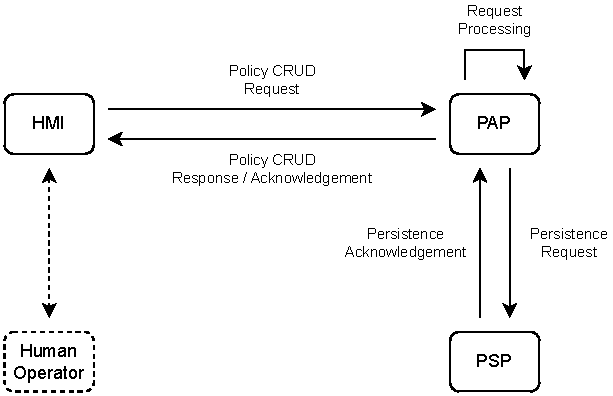
\includegraphics[width=0.75\linewidth]{figures/SABAAC_protocols_authorization_static.drawio.pdf}
        \caption{Exchanged messages of the static authorization process.
        % The process is initiated by a policy modification request of a human operator at a HMI. The involved PAP instance relies on a PSP to persist static authorizations or SABAAC policies. Requests to persist changes to static authorizations are communicated in the form of CRUD requests between the PAP and PSP.
        }
        \label{fig:sabaac_authorization_static}
    \end{figure}
    \item[Policy Exchange] After a policy is created, modified, or deleted during static authorization, it is shared with the PDPs via policy exchange.
    The policy exchange is an interaction between a PAP and a PDP.
    The interaction is either initiated by a PAP as a result of a static authorization, or on request of a PDP.

    If a static authorization triggers the policy exchange, the PAP sends a policy exchange message to a PDP.
    This type of policy exchange is referred to as incremental policy exchange., i.e., only newly created, modified, or removed policies are exchanged.
    The incremental policy exchange is shown in \autoref{fig:sabaac_authorization_dynamic_policyexchange_incremental}.

    A policy exchange containing all relevant policies can be initiated by a PDP by sending a policy exchange request to a PAP.
    This type of policy exchange is referred to as complete policy exchange.
    The complete policy exchange is shown in \autoref{fig:sabaac_authorization_dynamic_policyexchange_complete}.
    \begin{figure}
        \centering
        \begin{subfigure}[t]{0.48\linewidth}
            \centering
            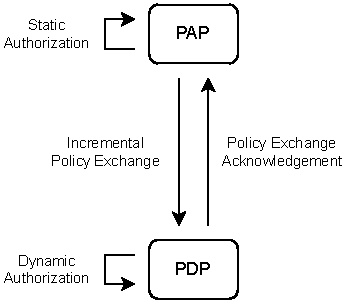
\includegraphics[width=\linewidth]{figures/SABAAC_protocols_authorization_dynamic_policyexchange_incremental.drawio.pdf}
            \caption{Incremental policy exchange procedure initiated by the static authorization of a PAP.}
            \label{fig:sabaac_authorization_dynamic_policyexchange_incremental}
        \end{subfigure}
        \hfill
        \begin{subfigure}[t]{0.48\linewidth}
            \centering
            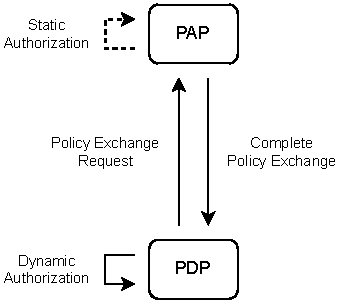
\includegraphics[width=\linewidth]{figures/SABAAC_protocols_authorization_dynamic_policyexchange_complete.drawio.pdf}
            \caption{Complete policy exchange procedure initiated by a policy exchange request of a PDP.}
            \label{fig:sabaac_authorization_dynamic_policyexchange_complete}
        \end{subfigure}
        \caption{Exchanged messages of the policy exchange procedures.
        %The static authorization is a prerequisite for both policy exchange procedures. The policy exchange is an interaction between a PAP and a PDP either initiated by a static authorization or on request of the involved PDP. The policy exchange is a prerequisite for dynamic authorization at a PDP. A repeatedly executed dynamic authorization process may be initially triggered by a policy exchange.
        }
        \label{fig:sabaac_authorization_dynamic_policyexchange}
    \end{figure}
    \item[Dynamic Authorization] The dynamic authorization process is responsible for deriving an access decision from an access control policy at the PDP.
    The process, the involved components, and the occurring message exchanges are visualized in \autoref{fig:sabaac_authorization_dynamic}.
    \Cref{alg:dynamic_authorization} shows the steps of the dynamic authorization process executed by a PDP, i.e., the process of deriving an access control decision in a given system for each access control policy available to the PDP.
    Depending on the evaluation strategy used, the dynamic authorization might either be triggered automatically prior to an access request of a PEP, or be triggered by an access request.
    As discussed in \autoref{sec:approach:sabaac:policy}, the dynamic authorization process is based on the dynamic authorization function $E_{POL}: Policy \times System \rightarrow Decision$.
    Prior to the evaluation of the dynamic authorization function for a policy, the PDP fetches the auxiliary attributes from other system entities via attribute request messages.
    These entities respond to the attribute requests with attribute resolution messages.
    As soon as the auxiliary attributes of a policy are available at the PDP, the dynamic authorization function $E_{POL}$ is evaluated.
    \begin{algorithm}
        \caption{Dynamic authorization process of a PDP deriving an access control decision for each access control policy in a given system.}
        \label{alg:dynamic_authorization}
        \begin{algorithmic}
        \Function{DynamicAuthorization}{$Policies$, $System$}
            \Let{$Decisions$}{$\left\{\,\right\}$} \Comment{Initialize an empty set of access decisions}
            \Let{$ATT_{System}$}{$\left\{\,\right\}$} \Comment{Initialize an empty system state}
            \\
            \ForIn{$\rho = (action_{\rho}, flow_{\rho}, auxiliary_{\rho})$}{$Policies$}
                \Let{$ATT_{auxiliary_{\rho}}$}{$\left\{\,\right\}$} \Comment{Initialize the auxiliary attributes of policy $\rho$}
                \ForIn{$a_i$}{$auxiliary_{\rho}$}
                    \LineComment{Request the attribute values for $a_i \in auxiliary_{\rho}$ from the system}
                    \Let{$ATT_{a_i}$}{\Call{ResolveAttributes}{$a_i, System$}}
                    \Let{$ATT_{auxiliary_{\rho}}$}{$ATT_{auxiliary_{\rho}} \cup ATT_{a_i}$}
                \EndFor
                \\
                \LineComment{Add the auxiliary attributes of policy $\rho$ to the current system state $ATT_{System}$}
                \Let{$ATT_{System}$}{$ATT_{System} \cup ATT_{auxiliary_{\rho}}$}
                \\
                \LineComment{Derive an access decision from policy $\rho$ \& the current system state $ATT_{System}$}
                \Let{$Decisions$}{$Decisions \cup E_{POL}(\rho, ATT_{System})$}
            \EndFor
            \State \Return $Decisions$
        \EndFunction
        \end{algorithmic}
    \end{algorithm}
    \begin{figure}
        \centering
        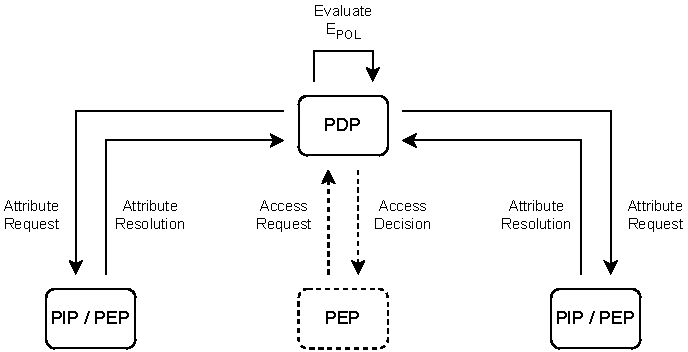
\includegraphics[width=0.9\linewidth]{figures/SABAAC_protocols_authorization_dynamic.drawio.pdf}
        \caption{Exchanged messages of the dynamic authorization process.
        }
        \label{fig:sabaac_authorization_dynamic}
    \end{figure}
\end{description}

\subsection{Delegated Attribute-Based Access Control Protocol}
\label{sec:approach:sabaac:accesscontrol}
In the following section, we discuss the delegated attribute-based access control protocol of the SABAAC approach.
The goal of the access control protocol is the request, exchange, and enforcement of access control decisions.
The devices of a SAS, including IEDs and MUs, neither request nor enforce the access control decisions but delegate these tasks to trusted PEP instances.
The access control decisions result from the dynamic authorization process discussed in \autoref{sec:approach:sabaac:authorization}.
Since the PDP instances execute the dynamic authorization, the provisioning of access control decisions is delegated to the PDP instances as well.

The delegated attribute-based access control protocol comprises reliable and unreliable services.
These services are provided by PDPs and used by PEPs.
Since the services provided by the protocol are directly related to domain-specific messages, the protocol is part of the CASC-SAS data path.
Accordingly, the occurring message exchanges are time-critical and traffic-intensive.
As with the delegated attribute-based authorization protocol, the access control protocol uses signing and verification services provided by CASA to safeguard the integrity and authenticity of messages.
Furthermore, messages of the protocol are sequenced, as defined by security policy IV in \autoref{sec:approach:security_policies}, to protect the protocol against intentional or accidental re-ordering, replaying, and delaying of messages.
The parts of the protocol that guarantee the delivery of messages, use an ARQ approach with positive acknowledgements and timeout-based retransmissions to achieve reliable message exchange.
As the message exchanges of the protocol are time-critical, negative acknowledgements are used in addition to timeout-based retransmissions to indicate errors and trigger retransmissions.

% The access control protocol of the SABAAC approach uses digitally signed and partially acknowledged message exchange.
% As with the authorization protocol, it uses digital signatures and verification provided by CASA to verify the integrity and authenticity of messages.
% To exchange messages on the control path, the access control protocol relies on reliable transport services provided by the message exchange layer.
% Data path message exchange of the access control protocol relies on either reliable or unreliable transport services depending on requirements such as message integrity and congestion tolerance.
% Moreover, the protocol is based on discontinuous message-based communication as well as continuous session-based communication at the cybersecurity layer.
% The access control sessions are initialized at the sending and receiving entities prior to the exchange of domain-specific messages.

% The security of the access control protocol is vulnerable to three distinct threats.
% Due to its communication architecture the protocol is vulnerable to replay, Denial-of-Service (DoS), and collusion attacks.
% Replay of messages represents a threat for session-based and message-based communication.
% Session-based communication of the protocol uses session identifiers and sequence numbers to provide replay protection.
% Message-based communication employs timestamp-based replay protection, similar to the discontinuous communication used by the authorization protocol.
% DoS attacks represent a threat for session-based communication due its stateful concept including session initialization and management.
% To mitigate malicious DoS attacks and DoS due to configuration and system errors, the access control uses a soft-state session-based message exchange.
% Accordingly, the session states used by the communicating entities have to be refreshed periodically and unused or invalid states are deleted.
% As a consequence, devices may not make assumptions about the current state of other devices.
% Moreover, a device has to handle session state exceptions via reinitialization of access control sessions.
% The third type of security threat is the collusion of malicious PDP and PEP instances.
% A collusion attack occurs if a PDP forges an access decision that is used by a PEP to access a protected object in an unauthorized manner.
% To mitigate collusion and reduce the trust in a PDP, a PEP can use server-aided access decision verification.
% Therefor, a PEP can request the verification of a PDP access decision from another PDP.

The workflow of the access control protocol is divided into three mandatory phases and an optional verification phase.
The phases of the access control protocol are defined as follows:
\begin{description}
    \item[Access Request] The access request represents the initial phase of the access control procedure.
    The goal of this phase is the exchange of an access decision between a PDP and PEP.
    The access request phase is initiated by a PEP on behalf of a domain subject.
    Depending on the evaluation strategy used, the PEP either sends an access request to a PDP before or after a domain-specific request arrives at the PEP.
    On receipt of an access request, the PDP verifies the request, fetches the requested access decision from its cache or derives it via dynamic authorization, and returns the access decision to the requesting PEP.

    To identify the requested access decision and the corresponding access control policy at the PDP, the PEP appends a set of flow attributes $ATT_{f} \subseteq f$ of a data frame flow $f$ to the access request.
    The PDP uses these flow attributes to evaluate the flow patterns of the available access control policies.
    Consequently, the flow attributes are used by the PDP to identify all applicable policies.
    The PDP returns the access decision of the applicable access control policy with the most specific flow pattern match.
    As discussed in \autoref{sec:approach:sabaac:policy}, if multiple conflicting access control policies are applicable, the composite decision of the corresponding access decisions can be used to resolve the conflict.
    If no access control policy is applicable, the PDP returns a default access decision $d_{Default}$ that matches the flow attributes $ATT_{f}$ exactly.
    Since the default action of SABAAC is $DENY$, the default access decision is $d_{SABAAC} = \{flow_{ATT_{f}}, DENY, \emptyset, validity_{Default}\}$.

    \item[Session Initialization] The session initialization is executed by a PEP that is granted access during the access request phase.
    To initialize an access control session, a PEP sends a session initialization request to another PEP.
    The request has to contain a PDP-signed granted access decision.
    The PEP may send the initialization request along with domain-specific data by piggybacking a payload exchange request.
    A more detailed examination of the piggybacking approach is provided below.
    On receipt of an initialization request, a PEP may optionally use server-aided access decision verification that is further discussed in the following section.
    If a received initialization request is valid, the PEP initializes a session state by adding the encapsulated access decision to an internal set of access decisions for incoming messages.
    Furthermore, the PEP sends a positive initialization acknowledgement and starts processing piggybacked domain-specific requests.
    If the request is invalid, the PEP sends a negative initialization acknowledgement and discards the piggybacked domain-specific request.

    A successful session initialization between two PEPs is shown in \autoref{fig:sabaac_accesscontrol_initialization}.
    Besides the session initialization procedure, the figure shows a preceding access request and a server-aided access decision verification at the receiving PEP.
    Additionally, the shown SABAAC components rely on computation requests for server-aided cryptography provided by the APEX protocol of CASA.
    \begin{figure}
        \centering
        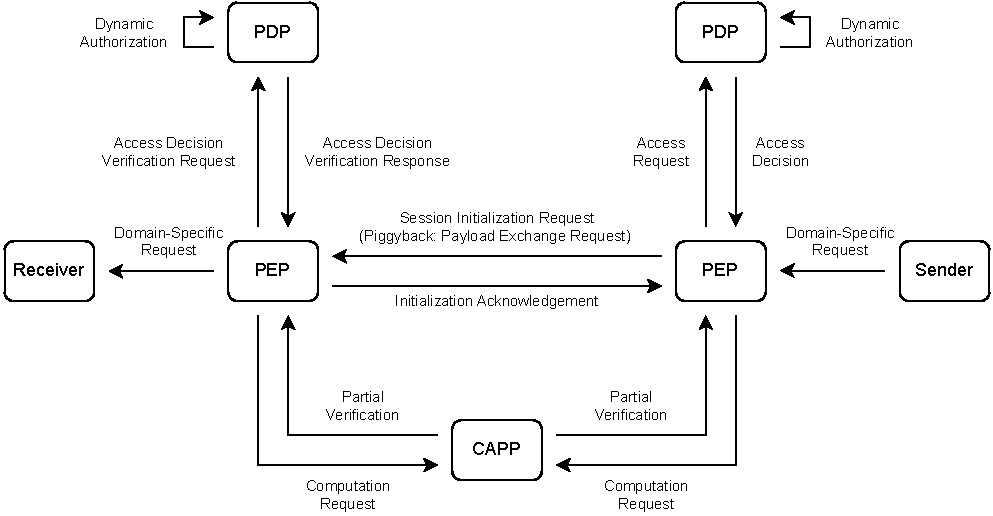
\includegraphics[width=1.0\linewidth]{figures/SABAAC_protocols_accesscontrol_initialization.drawio.pdf}
        \caption{Exchanged messages of an access request with unidirectional session initialization and access decision verification.
        % The access request procedure relies on an interaction between a PDP and a PEP and is a prerequisite for the session initialization. The session initialization relies on an interaction between two PEP instances. The receiver's PEP uses a server-aided access decision verification provided by a PDP to reduce the trust in another PDP. The shown SABAAC components, especially resource-constrained PEP instances, rely on the services provided by a CASA CAPP for SAV.
        }
        \label{fig:sabaac_accesscontrol_initialization}
    \end{figure}
    \item[Access Decision Verification] The optional server-aided access decision verification enables a PEP to verify received access decisions.
    This optional step is used to reduce the trust in a single PDP instance.
    To initiate the verification process, a PEP appends a PDP-signed access decision to an access decision verification request, and sends the request to another PDP.
    The PDP verifies the access decision and sends a positive or negative access decision verification response back to the PEP.
    \item[Payload Exchange] The payload exchange phase is the final phase of the access control protocol.
    The goal of the payload exchange phase is to securely exchange domain-specific requests or data between a sending and a receiving domain entity, i.e., between two SAS devices, such as IEDs or MUs.
    As the payload exchange is time-critical and traffic-intensive, delivery of messages cannot be guaranteed via positive acknowledgements and timeout-based retransmissions.
    Consequently, the service provided by the payload exchange phase is unreliable with regard to dropping of messages.
    However, the payload exchange phase relies on a Negative Acknowledgement (NACK) concept.
    A NACK is sent in case of an exception, thus acknowledgement implosions in multicast and broadcast communication scenarios are avoided.
    A received NACK may trigger a session re-initialization workflow at a PEP.

    The payload exchange is initiated by a domain entity via delivery of a domain-specific data frame to its PEP.
    On receipt of a domain-specific data frame $f$, the sender's PEP identifies all matching access control decisions $d_1, \dots, d_n$ by evaluating their flow patterns for data frame $f$.
    As in the access request phase and as discussed in \autoref{sec:approach:sabaac:policy}, the PEP uses the access decision of the applicable access control policy with the most specific flow pattern match, or a composite decision in case of a conflict.
    If no matching access decision is available, the PEP initiates an access request and session initialization procedure.
    As soon as the access decision is available, the PEP executes the decision enforcement function $E_{DEC}: Decision \times Frame \rightarrow (Action, Nexthop)$.
    If the access decision is granting, the PEP encapsulates the data frame in a payload exchange request, and forwards the request to each $PEP \in nexthop$.
    On receipt of the payload exchange request, the receiving PEP fetches the most specific access decision and evaluates $E_{DEC}$.
    If the access decision is granting and the receiving PEP is part of the $nexthop$ set, the encapsulated data frame is forwarded to the receiving domain entity.
    Otherwise, the payload exchange request is discarded.
    A successful unidirectional payload exchange between a sender and receiver is shown in \autoref{fig:sabaac_accesscontrol_payloadexchange}.
    The shown procedure relies solely on the interaction of PEP instances, with the exception of a computation request for server-aided cryptography on message receipt.
    \begin{figure}
        \centering
        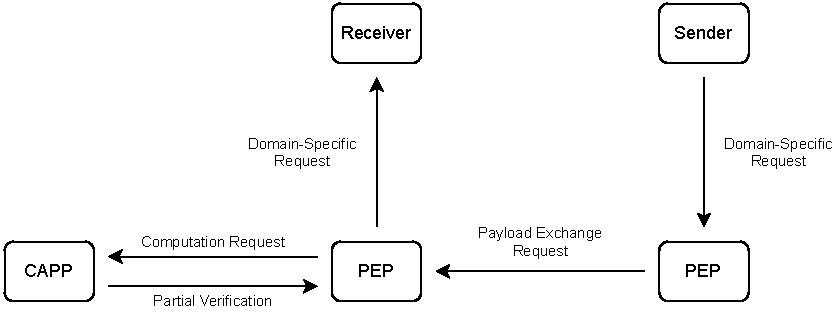
\includegraphics[width=0.9\linewidth]{figures/SABAAC_protocols_accesscontrol_payloadexchange.drawio.pdf}
        \caption{Exchanged messages of a unidirectional payload exchange procedure.
        % The procedure relies solely on the interaction of PEP instances, with the exception of a single server-aided CASA verification on message receipt.
        }
        \label{fig:sabaac_accesscontrol_payloadexchange}
    \end{figure}
    
    \item[Piggybacked Payload Exchange] Domain-specific communication is unidirectionally handled by the access control protocol of SABAAC.
    Consequently, a response to a domain-specific request is handled as independent message exchange by the PEPs.
    To reduce the overhead of session initialization handshaking, the requesting PEP may send the session initialization request along with a domain-specific data frame by piggybacking a payload exchange request.
    The processing of piggybacked payload exchange requests starts as soon as the corresponding initialization request is processed.
    The usage of piggybacking decreases the required time until a domain-specific request arrives at a PEP.
    Since session initialization requires at least one RTT for handshaking, a non-piggybacked domain-specific request is delayed by at least one RTT.
    As session initialization is handled unidirectionally, the handshaking leads to a delay of at least two RTTs for bidirectional domain-specific communication.

    A simplified session initialization procedure between two PEPs is shown in \autoref{fig:sabaac_accesscontrol_initialization_rtt}.
    A session initialization procedure without piggybacking is shown in \autoref{fig:sabaac_accesscontrol_initialization_rtt_nopiggyback}, whereas \autoref{fig:sabaac_accesscontrol_initialization_rtt_piggyback} shows the same payload exchanges using piggybacked requests.
    Three RTTs are the minimum time until a response to a domain-specific request can be received if no piggybacking is used.
    This three RTT delay consists of one RTT for forward session initialization, a half RTT for the forward payload exchange request, one RTT for backward session initialization, and a half RTT for the backward payload exchange request.
    The use of piggybacking reduces the minimum time required to deliver the first payload exchange request from one and a half RTTs to a half RTT under the assumption of symmetric transmission times.
    The minimum time until a response is delivered for the initial payload exchange request is reduced from three RTTs to a single RTT.
    After the bidirectional initialization of sessions, the minimum time required for a bidirectional payload exchange equals one RTT in both scenarios.
    \begin{figure}
        \centering
        \begin{subfigure}[t]{0.48\linewidth}
            \centering
            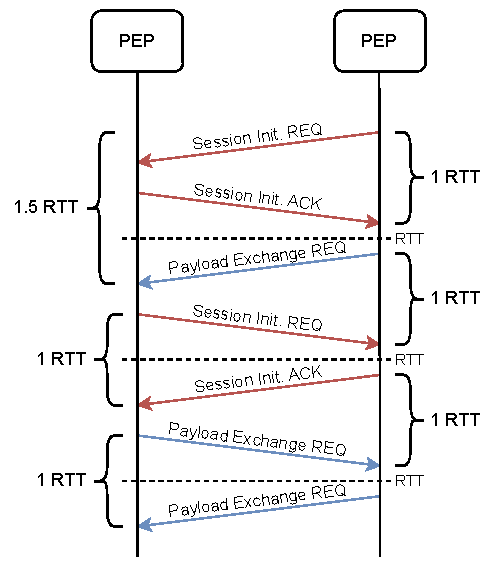
\includegraphics[width=\linewidth]{figures/SABAAC_protocols_accesscontrol_initialization_rtt_nopiggyback.drawio.pdf}
            \caption{Bidirectional session initialization and payload exchange without piggybacking.}
            \label{fig:sabaac_accesscontrol_initialization_rtt_nopiggyback}
        \end{subfigure}
        \hfill
        \begin{subfigure}[t]{0.48\linewidth}
            \centering
            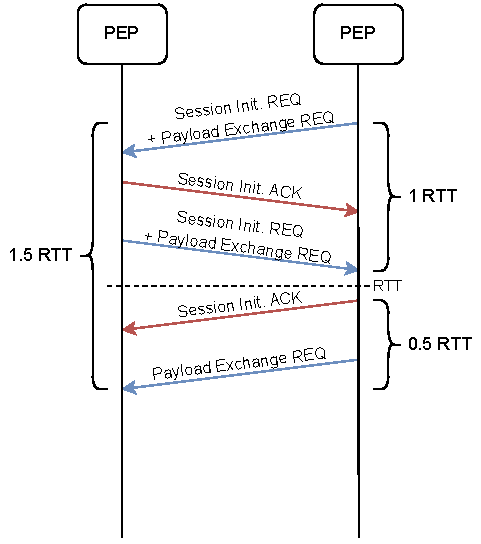
\includegraphics[width=\linewidth]{figures/SABAAC_protocols_accesscontrol_initialization_rtt_piggyback.drawio.pdf}
            \caption{Bidirectional session initialization and payload exchange with piggybacking.}
            \label{fig:sabaac_accesscontrol_initialization_rtt_piggyback}
        \end{subfigure}
        \caption{Protocol sequence diagrams of bidirectional session initialization and message exchange.
        % Protocol sequence diagrams showing a simplified piggybacking and non-piggybacking initialization of sessions for bidirectional message exchange and payload exchange between two PEP instances. For RTT comparison purposes, the semantically identical session initialization handshakes and message exchanges are shown without and with piggybacking of payload exchange requests. The use of piggybacking reduces the minimum time required to deliver the first payload exchange request from two RTTs to a half RTT under the assumption of symmetric transmission times. The minimum time until a response is delivered for the initial payload exchange request is reduced from three RTTs to a single RTT. After the bidirectional initialization of sessions, the minimum time required for a bidirectional payload exchange equals one RTT for both scenarios.
        }
        \label{fig:sabaac_accesscontrol_initialization_rtt}
    \end{figure}
\end{description}

\section{Realization}
\label{sec:approach:realization}
In the following section, we discuss the realization of the CASC-SAS approach and its two core concepts CASA and SABAAC.
The approach and its two core concepts introduce components that are defined and discussed in \autoref{sec:approach:casa} and \autoref{sec:approach:sabaac}.
To employ the CASC-SAS approach in a SAS, these components have to be integrated into the system architecture of a newly constructed or retrofitted SAS.
The three-layered architecture of a SAS, as introduced in the IEC 61850 standards \cite{IEC61850P8}, is shown in \autoref{fig:substation_architecture}.
Our adaptation of the layered SAS architecture integrating the introduced components of the CASC-SAS approach is shown in \autoref{fig:casc_architecture}.
Any non-intermediate SAS devices that participate in a communication relationship must either support the CASC-SAS protocols or use the services provided by a PEP to secure occurring message exchanges according to the CASC-SAS security policies introduced in \autoref{sec:approach:security_policies}.
The components depicted in blue represent devices of a typical SAS, whereas the components depicted in red are introduced by the CASC-SAS approach.
The components with a color gradient represent SAS devices that have been adapted to support CASC-SAS concepts.

The employed components of CASA and SABAAC provide different types of services, and have to be deployed differently to correspond to the presented protocols.
Since the delegated attribute-based authorization protocol is part of the time-critical and traffic-intensive data path of CASC-SAS, the PEPs and PDPs have to be present locally in every adapted SAS.
Furthermore, at least one CAPP instance has to be present locally in a SAS to support query and computation transactions in a timely manner, i.e., to take the strict time constraints of SAS-internal low latency message exchanges into account.
The PAP and PSP may be centrally deployed, as the delegated attribute-based authorization protocol of SABAAC is part of the non-time-critical control path communication.
Consequently, while some components may be deployed centrally, other components have to be distributed to individual substations.
This leads to differing hardware requirements for the deployed components.
With the exception of PEP instances, the components provide their services by using a client-server pattern.
The PEP instances partially use a client-server pattern and partially provide their services in the form of a Bump-In-The-Wire (BITW) solution.
The services of the delegated attribute-based access control protocol at the PEPs are provided via BITW pattern.
Therefore, these services are invisible to the corresponding service consumers, i.e., to the SAS devices secured by the PEPs.
The BITW pattern is inspired by the security filter approach presented by \citeauthor{Ishchenko2018} \cite{Ishchenko2018}.
Taking the differing provision patterns and deployment structures into account, we propose the usage of performance-oriented server hardware for the PAP, PSP, PDP, and CAPP to avoid bottlenecks and mitigate the risk of accidental or malicious DoS.
For the highly distributed PEP instances, we propose the usage of inexpensive off-the-shelf hardware.
To reduce the trust in single component instances and achieve a fault-tolerant and scalable system, components can be deployed redundantly, as discussed for access decision verification in \autoref{sec:approach:sabaac:accesscontrol}.
\begin{figure}
    \centering
    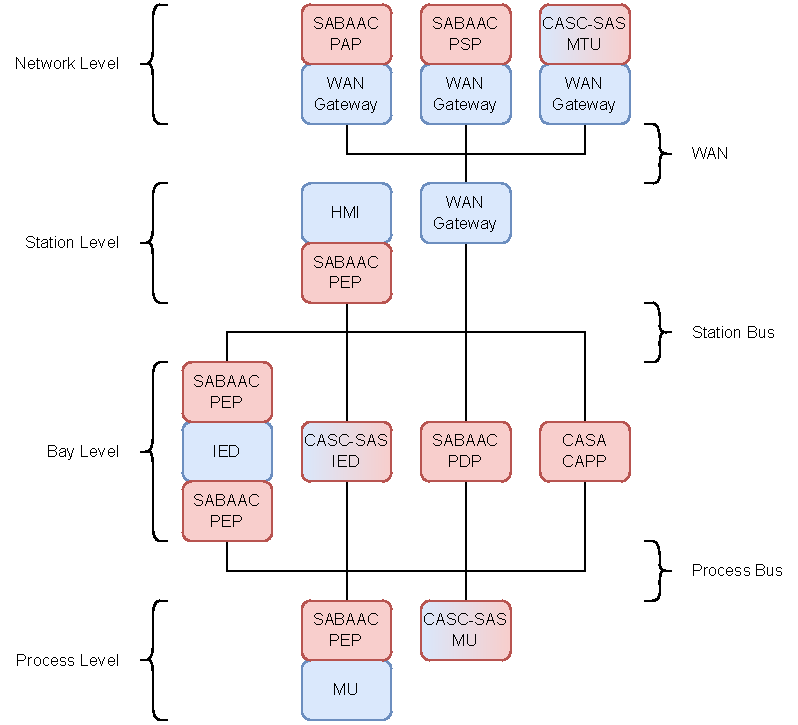
\includegraphics[width=1.0\linewidth]{figures/casc_architecture_color.drawio.pdf}
    \caption{Adaptation of the layered SAS architecture to the CASC-SAS approach.
    % The adaptation of the layered SAS architecture to the CASC-SAS approach entails a modification of the architecture to accommodate the additional components provided by CASC-SAS. The components depicted in blue represent elements of the SAS architecture, whereas the components depicted in red are introduced by the CASC-SAS approach. The components with a color gradient represent elements of the SAS architecture that have been adapted to support CASC-SAS concepts.
    }
    \label{fig:casc_architecture}
\end{figure}

\chapter{Evaluation}
\label{ch:evaluation}
In this section, we analyze and evaluate the CASC-SAS approach and discuss the findings of the evaluation.
The goal of the evaluation is to derive quantitative and qualitative characteristics of the approach.
These characteristics are used to verify the applicability of the approach in the presented field of application, i.e., the employment of the approach in newly constructed or retrofitted substations.
Furthermore, the characteristics are used to identify limitations and future directions of the approach.

\section{Method}
The evaluation is performed theoretically as well as experimentally.
For the theoretical parts of the evaluation, we employ proofs to demonstrate and guarantee certain characteristics of our approach.
The experimentally performed parts of the evaluation are based on a testbed implementation of our approach and the concepts discussed in \autoref{sec:approach:realization}.
The areas and metrics covered by the different parts of the evaluation are discussed in the following section.

\subsection{Evaluation Areas \& Metrics}
The evaluation of our approach is based on the goal-question-metric (GQM) approach \cite{Basili84,Basili92}.
The GQM approach aims to analyze whether an overall goal was achieved by answering a set of questions that represent the different areas of interest of the evaluation.
These questions are answered by deriving and evaluating quantitative and qualitative metrics.
The evaluation of the CASC-SAS approach covers three areas of interest.
The three areas of interest, i.e., questions to be answered, and their corresponding metrics are defined below:
\begin{description}
    \item[Goal:] Protect the time-constrained and traffic-intensive communication of a newly constructed or retrofitted SAS against domain-typical adversaries and attacks.
    \begin{description}
        \item[Question: Security] Does CASC-SAS provide security against typical SAS adversaries and attacks?
        \begin{description}
            \item[Metric:] Which security, safety, and availability requirements can be satisfied by deploying the approach in a SAS?
            \item[Metric:] Which adversary and system characteristics are assumed?
            \item[Metric:] Which attacks can be mitigated, and how can these attacks be mitigated with regard to their corresponding mitigation strategy?
            \item[Metric:] How does the attack surface of the SAS change?
        \end{description}
        \item[Question: Performance] Is CASC-SAS capable of securing time-constrained and traffic-intensive communication of an SAS in an efficient and scalable manner?
        \begin{description}
            \item[Metric:] Which performance requirements can be satisfied by deploying the approach in a SAS?
            \item[Metric:] Which communication characteristics are assumed?
            \item[Metric:] Which message types are supported?
            % \item Resistance against network exceptions including congestion, delay, jitter, duplicated packets, lost packets, and out-of-order packet delivery
        \end{description}
        \item[Question: Compatibility] Is CASC-SAS a viable solution to enhance the security of newly constructed or retrofitted substations?
        \begin{description}
            \item[Metric:] Which compatibility requirements can be satisfied by deploying the approach in a SAS?
            \item[Metric:] Which device requirements are assumed?
            \item[Metric:] What are the additional costs for SAS construction and retrofitting?
            \item[Metric:] Is the approach feasible with regard to SAS retrofitting?
            % \item Cost-benefit efficiency compared to alternative approaches
        \end{description}
    \end{description}
\end{description}

\subsection{Testbed}
To analyze and evaluate the integration of our approach into the SAS architecture, as discussed in \autoref{sec:approach:realization}, we implemented the approach in hardware and software as a testbed.
The software is implemented component-wise using object-oriented high-level programming languages.
The components are primarily implemented using the programming languages Java and Kotlin.
The software implementation of our approach is published open source on GitHub \cite{gitcasc} under the European Union Public Licence (EUPL) \cite{eupl}.
The implementation is divided into three main packages.
These packages, their sub-packages, and the package interrelationships are shown in \autoref{fig:casc_package_structure}.
The common package contains functionalities that are required by all other parts of the implementation.
Among others, the common package contains classes and interfaces related to message ingress and egress, message serialization, concurrency, and cryptography.
The second package and its sub-packages are dedicated to the CASA components and protocols.
The third package and its sub-packages are dedicated to the SABAAC components and protocols.
To avoid circular dependencies between the packages and achieve loose coupling of components, we employ the dependency inversion principle by using interfaces.
\begin{figure}
    \centering
    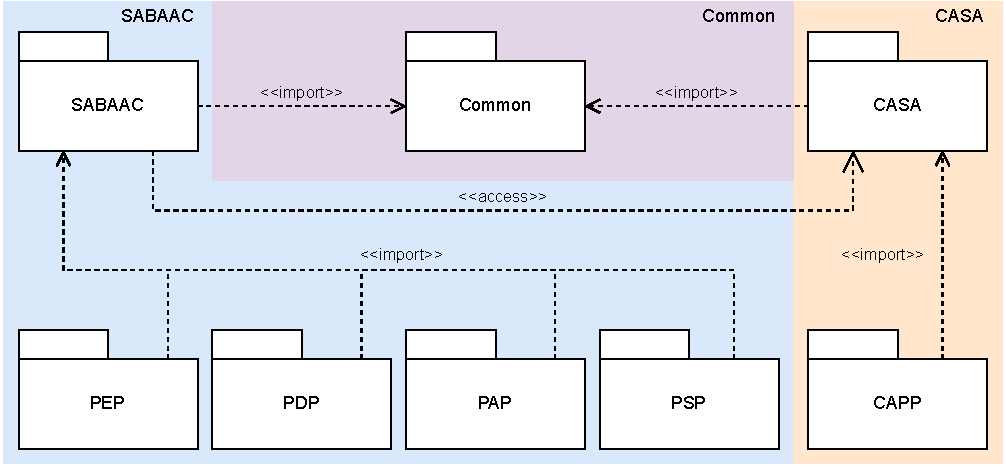
\includegraphics[width=0.9\linewidth]{figures/package_structure.drawio.pdf}
    \caption{Structural package diagram of the CASC-SAS testbed implementation.}
    \label{fig:casc_package_structure}
\end{figure}

To be able to conduct experiments while taking the behavior of physical network communication into account, we transformed the software implementation into a physical system by deploying the SABAAC and CASA components to hardware.
In contrast to deterministic software-based analysis, the testbed evaluation results are practice-oriented and transferable to the SAS domain.
The conceptual topology of our testbed network is visualized in \autoref{fig:evaluation_test_bed}.
The components depicted in blue represent domain-specific devices of an SAS, including IEDs and MUs.
%and computers that mimic the behavior of domain-specific devices of an SAS
The components depicted in yellow represent intermediate network devices for frame and datagram forwarding on the data link layer and network layer.
The components depicted in red are part of the CASC-SAS approach.
The specific hardware used for the experiments is discussed for each experiment individually in the following sections.
\begin{figure}
    \centering
    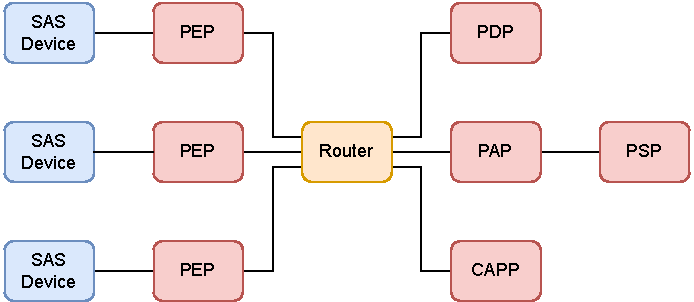
\includegraphics[width=0.8\linewidth]{figures/network_testbed_color.drawio.pdf}
    \caption{Conceptual network topology of the CASC-SAS testbed.}
    \label{fig:evaluation_test_bed}
\end{figure}
%The specific hardware used for the experiments is shown in \autoref{tab:testbed_hardware}.
%We conducted the experiments using a single TTP server that provided the PDP, PAP, PSP, and CAPP services.
%For experiments without real SAS devices, we deployed the PEPs as well as machines that mimic the behavior of domain-specific SAS devices to individual off-the-shelf Raspberry Pi 5 computers.
%For experiments with real IEDs and MUs, only the PEPs were deployed to Raspberry Pi 5 computers.
%
%The simulation and testbed strategy have differing advantages and disadvantages.
%On the one hand, the simulation strategy has the advantage of repeatability and reproducibility due to deterministic behavior, whereas the behavior of the testbed is non-deterministic.

\section{Security Analysis}
In this section, we conduct an analysis of the security of the CASC-SAS approach and its core concepts CASA and SABAAC.
The primary objective of the security analysis is to demonstrate and guarantee certain security-related characteristics of the approach.
As the security analysis is performed theoretically, proofs will be provided demonstrating that the approach is able to mitigate adversarial attacks that endanger these security-related characteristics.
\begin{description}
    \item[Definition.] Unforgeability.\\
    Unforgeability ensures that no adversary can create a valid signature for a message under a policy unless their set of attributes satisfies the policy.
    Unforgeability is defined by using a game between a challenger and an adversary $\mathcal{A}$:
    \begin{itemize}
        \item Setup: The challenger runs the \texttt{Setup} algorithm to generate the public parameters $PK$ and the master secret key $MSK$.
        The public parameters are given to $\mathcal{A}$, while the $MSK$ is kept secret.

        \item KeyGen: $\mathcal{A}$ can query the \texttt{KeyGen} oracle to obtain private keys for sets of attributes of its choice.
        The challenger responds with the corresponding private keys.

        \item SignQueries: $\mathcal{A}$ can request signatures for messages and policies from the \texttt{Sign} oracle.
        The oracle returns valid signatures if the queried attributes satisfy the signing policy.

        \item Forgery: $\mathcal{A}$ outputs a forged signature $(M^*, T^*, \sigma^*)$ for a message $M^*$ and policy $T^*$.
        $\mathcal{A}$ wins if the following conditions hold:
        \begin{itemize}
            \item $\mathcal{A}$ did not request a signature on $(M^*, T^*)$ from the \texttt{Sign} oracle.
            \item $\mathcal{A}$ does not possess a private key whose attributes satisfy the policy $T^*$.
            \item The verification algorithm accepts $\sigma^*$ as a valid signature under $T^*$.
        \end{itemize}
    \end{itemize}

    \item[Definition.] Existential Unforgeability under Chosen-Message Attacks (EU-CMA).\\
    An adversary $\mathcal{A}$ is given access to public parameters, hash oracles, and a signing oracle.
    A scheme is secure if $\mathcal{A}$ cannot forge a valid signature $\sigma^*$ for a new message $M^*$ without knowing the signer's full private key.
    In other words, to create an existential forgery, i.e., create a valid pair of message and signature for a new message, an adversary carrying out a CMA can request valid signatures for any message of his choice \cite{Goldwasser1988}.
    The adversary's advantage in this game is its probability of generating a valid forgery.
    We say the ABS scheme is \textit{existentially unforgeable} if the adversary's advantage is negligible.

    \item[Theorem.] $\mathcal{S}_{CASA}$ is EU-CMA secure under the Computational Diffie-Hellman (CDH) assumption in the random oracle model.\\
    \textit{Proof.} After querying the signing oracle, assume $\mathcal{A}$ forges a signature $\sigma^*$ for $M^*$.
    The challenger interacts with $\mathcal{A}$ as follows:
    \begin{itemize}
        \item \textit{Setup}: The challenger generates the public system parameters $\rho$ and the hash oracles \( H_1, H_2, H_3 \) for \( \mathcal{A} \).
        The challenger also programs the random oracles \( H_1, H_2, H_3 \) to embed a CDH instance \( g_1^a \) and \( g_1^b \), where \( a, b \) are random exponents.
        \item \textit{HashQueries}: The challenger responds to \( H_1, H_2, H_3 \) queries with random values, ensuring consistency.
        \item \textit{SignQueries}: When $\mathcal{A}$ requests a signature on a message \( M \) under an access policy \( T \), the challenger computes the signature as:
        \[
            \sigma_i = ppk_i \cdot H_3(h)^{\chi_i},
        \]
        where $h = H_2(M || T)$.
        \item \textit{Forgery}: Eventually, the adversary outputs a forged signature $\sigma^*$ on a message $M^*$ under an access policy $T^*$.
        The challenger extracts the solution to the CDH problem $g_1^{ab}$ from the forged signature by exploiting the structure of the random oracle responses.
    \end{itemize}
    $\mathcal{A}$'s success in forging a signature implies the ability to solve the CDH problem.
    Since the CDH problem is assumed to be hard, $\mathcal{A}$'s advantage in breaking the scheme is negligible.
    Thus, the $\mathcal{S}_{CASA}$ scheme is secure under the EU-CMA model and under the assumption of the hardness of the CDH problem in the random oracle model.

    \item[Definition.] Collusion Attack.\\
    An adversary $\mathcal{A}$ colludes with a TTP and corrupted signers to derive private keys or forge valid signatures.
    The scheme is secure if such a collusion does not compromise honest signers and does not allow forgery.

    \item[Theorem.] $\mathcal{S}_{CASA}$ resists collusion attacks under the Discrete Logarithm Problem (DLP).\\
    \textit{Proof.} Suppose $\mathcal{A}$ colludes with the CAPP to derive $sk_i = (ppk_i, \chi_i)$, then the following steps are performed:
    \begin{itemize}
        \item The CAPP knows $ppk_i = H_1(ID_i || ATT_i)^{s}$.
        \item The signer independently chooses $\chi_i$ and the DLP ensures $\mathcal{A}$ cannot derive $\chi_i$.
        \item Without $\chi_i$, $\mathcal{A}$ cannot compute:
        \[
            \sigma_i = ppk_i \cdot H_3(h)^{\chi_i}.
        \]
    \end{itemize}
    Thus, collusion cannot compromise security.
    The $\mathcal{S}_{CASA}$ scheme is secure against collusion attacks.

    \item[Definition.] Message Replay.\\
    To perform a message replay, an adversary captures and repeats the messages exchanged between two or more network devices.
    The adversary aims to inject false data into the system, or disrupt the operation of the network devices.

    \item[Theorem.] CASC-SAS protects SAS devices against message replay attacks.\\
    \textit{Proof.} Suppose two SAS devices, $Alice$ and $Bob$, exchange messages over a network.
    We assume that an adversary $\mathcal{A}$, as introduced in \autoref{sec:approach:attacks}, is able to eavesdrop and replay the messages sent from $Alice$ to $Bob$, and vice versa.
    For the exchange of a message $m$ between $Alice$ and $Bob$, as shown in \autoref{fig:attack_message_replay}, the following steps are performed:
    \begin{itemize}
        \item $Alice$ sends the message $m$ to $Bob$ via $PEP_{Alice}$.
        \item To satisfy the security policies I and IV of CASC-SAS, $PEP_{Alice}$ encapsulates $m$ and a sequence number $seq_m$ in a packet $m' = (Alice, Bob, m, seq_m)$ and signs $m'$ to get $m'' = (m', \sigma_{m'})$.
        \item $PEP_{Alice}$ sends $m''$ to $PEP_{Bob}$ using the network. $PEP_{Bob}$ receives $m''$ from $PEP_{Alice}$, verifies the signature $\sigma_{m'}$, sets the last sequence number received from $PEP_{Alice}$ to $seq_m$, and delivers $m$ to $Bob$.
        \item $\mathcal{A}$ eavesdrops the message exchange, receives $m''$ at the same time as $PEP_{Bob}$, and replays $m''$ to $PEP_{Bob}$.
        \item $PEP_{Bob}$ receives $m''$ from $\mathcal{A}$. As $PEP_{Bob}$ already processed a packet from $PEP_{Alice}$ with sequence number $seq_m$, $m''$ is discarded.
    \end{itemize}
    $\mathcal{A}$ gains no advantage by replaying $m''$, as neither false data is injected into $Alice$ or $Bob$, nor is the operation of $Alice$ or $Bob$ disrupted.
    Thus, SAS devices are protected against message replay attacks.
    \begin{figure}
        \centering
        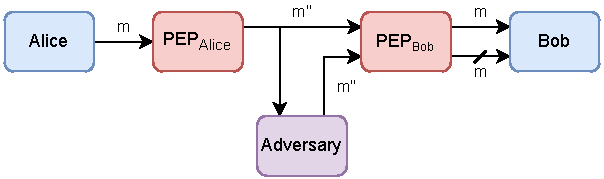
\includegraphics[width=0.75\linewidth]{figures/attack_message_replay.drawio.pdf}
        \caption{Malicious replay of a message exchanged between two PEP-protected SAS devices.}
        \label{fig:attack_message_replay}
    \end{figure}

    \item[Definition.] Message Forgery.\\
    To perform a message forgery, an adversary masquerades as a legitimate device to send malicious messages to other devices.
    By using message forgery, the adversary injects false data into the system, or disrupts the operation of devices.

    \item[Theorem.] CASC-SAS protects SAS devices against message forgery attacks.\\
    \textit{Proof.} Suppose two SAS devices, $Alice$ and $Bob$, exchange messages over a network.
    We assume that only the two devices have the necessary key material to sign and verify exchanged messages.
    As defined in \autoref{sec:approach:attacks}, we assume that an adversary $\mathcal{A}$ is able to initiate arbitrary message exchanges but is unable to bypass or break cryptographic procedures.
    To send a malicious message $m*$ from $\mathcal{A}$ to $Bob$, as shown in \autoref{fig:attack_message_forgery}, $\mathcal{A}$ has to perform the following steps:
    \begin{itemize}
        \item $\mathcal{A}$ creates a message $f$ of its choice.
        \item $\mathcal{A}$ encapsulates $f$ in a packet $m^* = ((Alice, Bob, f, seq_{m^*}), \sigma_{m^*})$, to masquerade as $PEP_{Alice}$.
        \item $\mathcal{A}$ sends $m^*$ to $PEP_{Bob}$.
        \item $PEP_{Bob}$ discards $m^*$ and does not deliver $f$ to $Bob$, as the signature $\sigma_{m^*}$ is not created by $PEP_{Alice}$.
    \end{itemize}
    Since only $PEP_{Alice}$ has the necessary key material to sign messages from $Alice$, $\mathcal{A}$ is unable to masquerade as $Alice$.
    Thus, SAS devices are protected against message forgery attacks.
    \begin{figure}
        \centering
        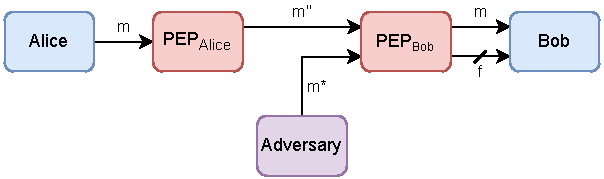
\includegraphics[width=0.75\linewidth]{figures/attack_message_forgery.drawio.pdf}
        \caption{Forgery of a message by masquerading as a PEP-protected SAS device.}
        \label{fig:attack_message_forgery}
    \end{figure}

    \item[Definition.] Message Modification.\\
    To perform a message modification, an adversary captures and alters messages exchanged between two or more network devices.
    Accordingly, message modification is a special type of message forgery that derives a malicious message from a captured message.

    \item[Theorem.] CASC-SAS protects SAS devices against message modification attacks.\\
    \textit{Proof.} Suppose two SAS devices, $Alice$ and $Bob$, exchange messages over a network.
    As with message forgery, we assume that only $Alice$ and $Bob$ have the necessary key material to sign and verify exchanged messages, and that an adversary $\mathcal{A}$ is unable to bypass or break cryptographic procedures.
    We assume that $\mathcal{A}$ performs the attack using a man in the middle approach, i.e., $Alice$ and $Bob$ are not directly connected and the exchanged messages traverse $\mathcal{A}$.
    The modification of a message $m$ from $Alice$ to $Bob$ using a man in the middle approach is shown in \autoref{fig:attack_message_modification}.
    To carry out a message modification attack, $\mathcal{A}$ has to perform the following steps:
    \begin{itemize}
        \item $Alice$ sends the message $m$ to $PEP_{Alice}$.
        \item To satisfy the security policies I and IV of CASC-SAS, $PEP_{Alice}$ encapsulates $m$ and a sequence number $seq_m$ in a packet $m' = (Alice, Bob, m, seq_m)$ and signs $m'$ to get $m'' = (m', \sigma_{m'})$.
        \item $PEP_{Alice}$ sends $m''$ unintentionally to $\mathcal{A}$ using the network.
        \item $\mathcal{A}$ modifies $m$ and encapsulates the modified message $f$ in a packet $m^* = ((Alice, Bob, f, seq_{m}), \sigma_{m})$.
        \item $\mathcal{A}$ sends $m^*$ to $PEP_{Bob}$.
        \item $PEP_{Bob}$ discards $m^*$ and does not deliver $f$ to $Bob$, as the signature $\sigma_{m'}$ does not match the content of $m^*$.
    \end{itemize}
    Since only $PEP_{Alice}$ has the necessary key material to sign messages from $Alice$, $\mathcal{A}$ is unable to renew the signature after modifying the encapsulated message.
    Thus, SAS devices are protected against message modification attacks.
    \begin{figure}
        \centering
        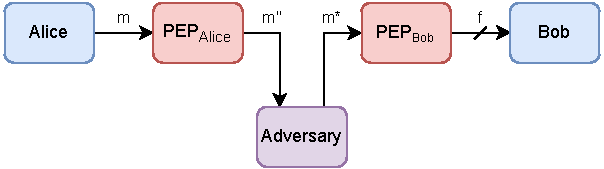
\includegraphics[width=0.75\linewidth]{figures/attack_message_modification.drawio.pdf}
        \caption{Malicious modification of a message exchanged between two PEP-protected SAS devices.}
        \label{fig:attack_message_modification}
    \end{figure}

    \item[Definition.] Time-Delay Attack.\\
    A time-delay attack is the intentional delaying of time-critical messages in a network.
    To perform a time-delay attack, a man in the middle adversary captures a message sent by a network device, and waits a certain time before forwarding it to the message receiver.
    By maliciously delaying exchanged messages, the adversary may either inject outdated data into the system or disrupt the operation of devices.

    \item[Theorem.] CASC-SAS protects SAS devices against time-delay attacks.\\
    \textit{Proof.} Suppose two SAS devices, $Alice$ and $Bob$, exchange messages over a network in the presence of an adversary $\mathcal{A}$, which performs a time-delay attack using a man in the middle approach.
    The performed time-delay attack is shown in \autoref{fig:attack_time_delay}.
    To carry out a message modification attack, $\mathcal{A}$ has to perform the following steps:
    \begin{itemize}
        \item $Alice$ sends the message $m$ to $PEP_{Alice}$.
        \item To satisfy the security policies I and IV of CASC-SAS, $PEP_{Alice}$ encapsulates $m$ with a timestamp-based sequence number $seq_m$ in a packet $m' = (Alice,\allowbreak Bob,\allowbreak m,\allowbreak seq_m)$ and signs $m'$ to get $m'' = (m', \sigma_{m'})$.
        \item $PEP_{Alice}$ sends $m''$ unintentionally to $\mathcal{A}$ using the network.
        \item $\mathcal{A}$ receives $m''$ and waits a certain time before sending it to $PEP_{Bob}$.
        \item $PEP_{Bob}$ discards $m''$ and does not deliver $m$ to $Bob$, as the sequence number $seq_m$ indicates that the packet was maliciously or accidentally delayed.
    \end{itemize}
    The delay of $m''$ would only be unnoticeable if $\mathcal{A}$ was able to update the sequence number.
    However, as only $PEP_{Alice}$ has the necessary key material to sign messages from $Alice$, $\mathcal{A}$ is unable to update the sequence number.
    Thus, SAS devices are protected against time-delay attacks.
    \begin{figure}
        \centering
        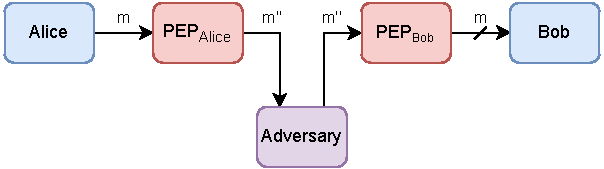
\includegraphics[width=0.75\linewidth]{figures/attack_time_delay.drawio.pdf}
        \caption{Malicious delaying of a message exchanged between two PEP-protected SAS devices.}
        \label{fig:attack_time_delay}
    \end{figure}
    %\item[Theorem.] CASC-SAS protects SAS devices against flooding attacks.\\
    %\textit{Proof.}
\end{description}

\section{Performance Analysis}
In this section, we conduct an analysis of the performance aspects of our approaches CASA and SABAAC.
The objective of the performance analysis is to demonstrate that our approaches are viable solutions to secure message exchanges, taking the strict time and resource constraints of a SAS into account.
For this purpose, we conducted an experimental estimation of message exchange latencies using our testbed implementation and off-the-shelf hardware.
In \autoref{sec:evaluation:performance:setup} the setup of the experiment is discussed in detail.
In \autoref{sec:evaluation:performance:procedure} we describe the procedure and results of the experiment.

\subsection{Experimental Setup}
\label{sec:evaluation:performance:setup}
The testbed of the performance analysis consists of eight devices.
The hardware devices used for the experiment are listed in \autoref{tab:performance_analysis_hardware}.
Two Raspberry Pi 5 were deployed to mimic domain entities that communicate with each other.
Another two Raspberry Pi 5 were used as PEPs protecting the domain entities.
A ThinkPad T480 provided the services of the PAP, PSP, PDP, and CAPP.
\begin{table}
    \centering
    \small
    \caption{Hardware used for the performance analysis testbed.}
    \label{tab:performance_analysis_hardware}
    \begin{tabular}{c c c c}
    \toprule
    Manufacturer & Device & Task & Amount\\
    \midrule
    % SAS Devices
    TP-Link & Omada ER605 & Gigabit Router & 1\\
    % CASA & SABAAC
    Raspberry Pi Ltd & Raspberry Pi 5 8GB & PEP \& Domain Entity & 4\\
    Lenovo & ThinkPad T480 & PDP/PAP/PSP/CAPP & 1\\
    Bechtle & ARTICONA Adapter & USB-A to RJ45 Adapter & 2\\
    \bottomrule
    \end{tabular}
\end{table}

The network topology of the devices used for the performance analysis is shown in \autoref{fig:performance_analysis_topology}.
The PAP, PSP, PDP, CAPP, and PEPs were connected to an industrial grade TP-Link Omada router using Ethernet over twisted-pair.
Each domain entity was connected to its corresponding PEP using Ethernet over twisted-pair, i.e., by using the on-board RJ45 Ethernet connector of the Raspberry Pi 5 domain entity.
However, since the Raspberry Pi 5 only possesses a single on-board RJ45 Ethernet connector, an additional USB-A to RJ45 Ethernet adapter had to be used for both PEPs in order to connect them to the router and to the domain entities.
\begin{figure}
    \centering
    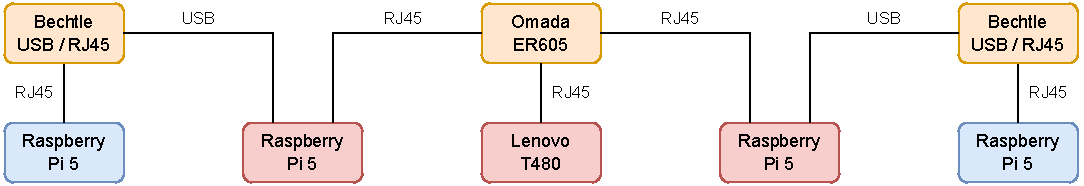
\includegraphics[width=1.0\linewidth]{figures/performance_evaluation_topology.drawio.pdf}
    \caption{Network topology of the performance analysis testbed.}
    \label{fig:performance_analysis_topology}
\end{figure}

\subsection{Procedure \& Results}
\label{sec:evaluation:performance:procedure}
To demonstrate the viability of our approach with regard to securing time critical message exchanges, we aimed to evaluate the extent to which our approach was capable of handling different message types.
For this purpose, we conducted an experiment to estimate the end-to-end communication latency of a message exchange between two domain entities.
The three message types that were considered for the evaluation are discussed in \autoref{sec:approach:system_model:communication:message_types} and listed in \autoref{tab:message_types}.

We realized the message exchange latency estimation by implementing a benchmark program and deploying it to the domain entities.
The benchmark program was implemented in Python.
The program is published open source on GitHub \cite{gitcasc} alongside the implementation of our approach.
The program estimated the end-to-end latency between the two domain entities based on the RTT of a bidirectional message exchange.
We chose UDP as a message exchange protocol for the experiment in order to avoid external latency influences, such as the flow control and congestion control of the Transmission Control Protocol (TCP).
To measure the RTT, the so-called active benchmark entity sent a timestamp to the passive benchmark entity.
The passive entity replied to the message with the received timestamp.
Thus, after receiving the response from the passive entity, the active entity was able to calculate the RTT by subtracting the received timestamp from the current timestamp.
As a consequence, no time synchronization was required between the domain entities.
Furthermore, under the assumption of symmetric transmission times, the accuracy of the RTT measurements only depended on the accuracy of the active entity's system clock.
To avoid RTT fluctuations or an offset caused by the router's buffering and forwarding strategy, messages were sent sequentially, i.e., the active entity waited for the arrival of a response before sending another timestamp message.

The procedure of the experimental latency estimation consisted of ten key events.
The sequence of events and the corresponding messages exchanged between the devices are shown in \autoref{fig:performance_analysis_latency_steps}.
To improve the readability of the shown message exchanges, the USB-A to RJ45 Ethernet adapters were omitted from the figure.
The steps of the experiment procedure are defined in the following:
\begin{description}
    \item[Step 1: Send Request]~\\
    At the initial state of the experiment, no domain-specific messages were exchanged between the devices.
    The necessary key material for signing and verification was already exchanged prior to the experiment.
    The PDP used the precomputed evaluation strategy for access policies, i.e., the access decisions were periodically refreshed and cached.
    The PEPs used a hybrid access decision evaluation strategy, i.e., access decisions were requested and cached as soon as they were needed.
    To initiate the end-to-end latency estimation, the active domain entity sent a UDP packet with its current system clock timestamp to the passive domain entity.

    \item[Step 2: Request Access]~\\
    As the active entity was protected by a PEP, the outgoing UDP packet was captured by the active entity's PEP.
    The PEP checked if an applicable and valid access decision for the packet-related data frames was available in its cache.
    If no applicable or valid access decision was available, the PEP sent an access request to the PDP.

    \item[Step 3: Exchange Request Payload]~\\
    As soon as an applicable and valid access decision was available, the active entity's PEP processed the UDP packet as discussed in \autoref{sec:approach:sabaac:accesscontrol} and sent a payload exchange request to the passive entity's PEP.

    \item[Step 4: Forward Request]~\\
    On receipt of a payload exchange request, the passive entity's PEP verified the request.
    After the request verification, the contained UDP packet was forwarded to the passive domain entity.

    \item[Step 5: Send Response]~\\
    On receipt of the UDP packet, the benchmark program of the passive domain entity extracted the timestamp, created a new UDP packet containing the same timestamp, and sent the new UDP packet to the active domain entity.

    \item[Step 6: Request Access]~\\
    As the passive entity was protected by a PEP, the outgoing UDP packet was captured by the passive entity's PEP.
    The PEP requested and enforced the access decision for the packet as discussed in the second step.

    \item[Step 7: Exchange Response Payload]~\\
    As soon as an applicable and valid access decision was available, the passive entity's PEP processed the UDP response packet and sent a payload exchange request to the active entity's PEP.

    \item[Step 8: Forward Response]~\\
    On receipt of a payload exchange request, the active entity's PEP verified the request and forwarded the contained UDP response packet to the active entity.

    \item[Step 9: Estimate RTT]~\\
    The benchmark program of the active domain entity extracted the timestamp from the response packet and calculated the RTT of the packet by subtracting the received timestamp from the current system clock timestamp.
    To compensate for fluctuations in the RTT measurements and to increase the confidence in the RTT estimation, the active entity repeated the RTT measurement procedure.
\end{description}
\begin{figure}
    \centering
    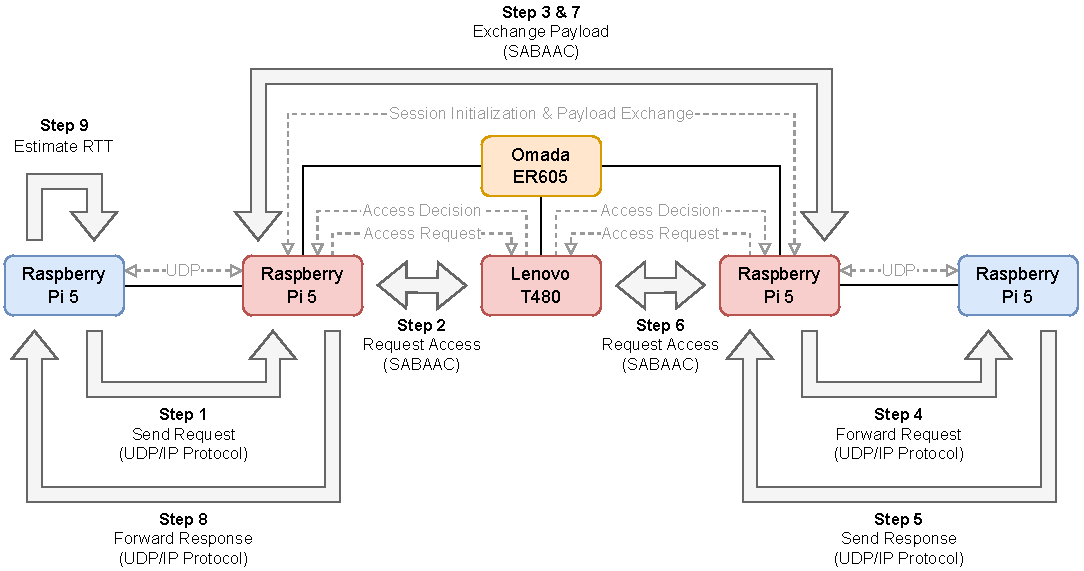
\includegraphics[width=1.0\linewidth]{figures/performance_evaluation_steps.drawio.pdf}
    \caption{Sequence of events of the experimental message exchange latency estimation.}
    \label{fig:performance_analysis_latency_steps}
\end{figure}

The results of the latency estimation experiment are shown in \autoref{tab:rtt_metrics} and \autoref{tab:rtt_share}.
The results are published open source on GitHub \cite{gitcasc} alongside the implementation of our approach.
Since CASA is an algorithm-agnostic approach, we conducted the message exchange latency estimation procedure for six different authentication algorithms.
For each of the authentication algorithms, the benchmark program sent 1000 sequential packets to estimate the RTT.
Based on the measurements, we calculated the arithmetic mean, median, standard deviation, and extrema-related values for each experiment.
Furthermore, we calculated the throughput of the PEPs in Packets Per Second (PPS), and the cumulative share of the 1000 packets in the three message types listed in \autoref{tab:message_types}.

To measure the latency offset caused by packet capturing and forwarding, we performed the initial latency estimation without authorizations, i.e., neither access control nor authentication were used.
From this data, we can see that a bidirectional message exchange between two domain entities requires 1.809 ms on average, which leads to a PEP throughput of 528.2 sequential PPS.
Without authentication, authorization, and access control in place, the measured RTTs are consistent, and each bidirectional message exchange was finished in less than 6 ms RTT, which is required to support the low latency message type.

To measure the influence of the authorization and access control, we performed a latency estimation with authorization and access control but without authentication.
For this purpose, we implemented a so-called no-operation authenticator, which processed the packets without signing or verifying them.
The measurements of the RTTs with the no-operation authenticator show that the authorization and access control workflow of SABAAC leads to an RTT increase of 1.1 ms on average.
Moreover, the increased range of minimum and maximum time indicates that SABAAC leads to an increase in RTT fluctuation.

In order to evaluate the performance of our approach in combination with symmetric cryptography, we performed a latency estimation for HMAC authentication based on SHA-512.
The results show that 99.8 \% of the message exchanges were finished in less than 6 ms RTT.
The remaining two packets or 0.2 \% of the 1000 packets satisfied the 20 ms time constraint of the medium latency message type.
By employing HMAC authentication, CASA and SABAAC achieved a throughput of 289.1 PPS at the PEPs.

To evaluate the performance of our approach in combination with PKC, we conducted latency estimations for three PKC algorithms.
For the latency estimations we chose the Ed25519 algorithm, which is an elliptic-curve digital signature algorithm, RSA-2048, and our $S_{CASA}$ signature scheme.
All three PKC approaches did not satisfy the time constraint of the low latency message type.
Ed25519 and RSA satisfied the time constraint of the medium latency message type.
$S_{CASA}$ was able to finish 99.8 \% of the message exchanges within the time constraints of the high latency message type, i.e., in less than 500 ms.
The data indicates that the RTTs of the PKC approaches are subject to fluctuations with higher magnitude compared to the fluctuations caused by SABAAC and symmetric cryptography.
Furthermore, the throughput of the PEPs was reduced by more than 70 \% compared to the HMAC authentication.
\begin{table}
    \centering
    \small
    \caption{Results of the RTT estimation based on 1000 measurements per authentication algorithm.}
    \label{tab:rtt_metrics}
    \begin{tabular}{c c c c c c c c}
    \toprule
    Authentication & Mean & Median & Deviation & \multicolumn{4}{c}{Extrema}\\
    \cmidrule(lr){5-8}
    & $\bar{x}$ & $\widetilde{x}$ & $\sigma$ & Min & Max & Range & Mid-Range\\
    \midrule
    Unauthorized    & 1.809 & 1.799 & 0.067 & 1.704 & 2.400 & 0.696 & 2.052 \\
    Unauthenticated & 2.937 & 2.924 & 0.146 & 2.808 & 4.213 & 1.405 & 3.511 \\
    HMAC            & 3.342 & 3.279 & 0.507 & 2.779 & 6.695 & 3.915 & 4.736 \\
    Ed25519        & 11.096 & 11.224& 1.591 & 9.537 & 31.971& 22.434 & 20.754 \\
    RSA-2048       & 12.703 & 12.034& 1.179 & 11.741& 16.804& 5.063 & 14.273 \\
    $S_{CASA}$    & 119.851 &113.127&28.534 &111.385&509.392&398.007&310.389\\
    \bottomrule
    \end{tabular}
\end{table}
\begin{table}
    \centering
    \small
    \caption{Throughput and cumulative message type share of the analyzed authentication algorithms.}
    \label{tab:rtt_share}
    \begin{tabular}{c c c c c}
    \toprule
    Authentication & Throughput & \multicolumn{3}{c}{Cumulative Share in Message Types}\\
    \cmidrule(lr){3-5}
     & & Low Latency & Medium Latency & High Latency\\
     & & $\leq 6~ms$ & $\leq 20~ms$ & $\leq 500~ms$\\
    \midrule
    Unauthorized    & 528.2 PPS & 1000 (100 \%) & 1000 (100 \%) & 1000 (100 \%) \\
    Unauthenticated & 328.2 PPS & 1000 (100 \%) & 1000 (100 \%) & 1000 (100 \%) \\
    HMAC            & 289.1 PPS &  998 (99.8 \%)& 1000 (100 \%) & 1000 (100 \%) \\
    Ed25519         &  88.9 PPS &    0 (0 \%)   &  998 (99.8 \%)& 1000 (100 \%) \\
    RSA-2048        &  77.4 PPS &    0 (0 \%)   & 1000 (100 \%) & 1000 (100 \%)\\
    $S_{CASA}$      &   8.2 PPS &    0 (0 \%)   &    0 (0 \%)   &  998 (99.8 \%)\\
    \bottomrule
    \end{tabular}
\end{table}

\section{Compatibility Analysis}
In this section, we conduct an analysis of the compatibility aspects of our approaches CASA and SABAAC.
The objective of the compatibility analysis is to demonstrate that our approach is a viable solution to enhance the communication security in a newly constructed or retrofitted substation.
Accordingly, the compatibility analysis serves the purpose of demonstrating that the SAS behavior and functionality is not influenced by our approach, and that SAS devices protected by CASA and SABAAC are able to provide their services and exchange information.
For this purpose, we conducted a laboratory-based experimental demonstration of applicability with industrial SAS devices.
In \autoref{sec:evaluation:compatibility:setup} the setup of the experiment is discussed.
In \autoref{sec:evaluation:compatibility:procedure} we describe the procedure and results of the experiment.

\subsection{Experimental Setup}
\label{sec:evaluation:compatibility:setup}
In total twelve devices were used to set up the experiment.
The hardware devices used for the experiment are listed in \autoref{tab:lab_hardware}.
Four of these devices were industrial SAS devices, including a MU from General Electric, an IED from ABB, an I/O box from Siemens, and a circuit breaker.
Additionally, a relay test device from Omicron was used to generate three-phase electric power, which was measured by the MU to generate SV frames.
Besides these five SAS-related devices, two Raspberry Pi 5 were used as PEPs.
A ThinkPad T480 provided the services of the PAP, PSP, PDP, and CAPP.
\begin{table}
    \centering
    \small
    \caption{Hardware used for the laboratory-based experimental demonstration of applicability.}
    \label{tab:lab_hardware}
    \begin{tabular}{c c c c c c}
    \toprule
    Manufacturer & Device & Task & SAS & CASC-SAS\\
    \midrule
    % SAS Devices
    General Electric & Reason MU320 & Process Bus Merging Unit & X & \\
    ABB & REL670 & Intelligent Electronic Device & X & \\
    Siemens & SIPROTEC 5 6MD84 & Input/Output Box & X & \\
    Hirschmann & MACH & Managed Ethernet Switch & X & \\
    Hirschmann & RSP35 & Managed Ethernet Switch & X & \\
    OMICRON & CMC 356 & Universal Relay Test Set & X & \\
    / & Circuit Breaker & Electrical Grid Switch & X & \\
    % CASA & SABAAC
    Raspberry Pi Ltd & Raspberry Pi 5 8GB & PEP & & X \\
    Lenovo & ThinkPad T480 & PDP/PAP/PSP/CAPP & & X \\
    Bechtle & ARTICONA Adapter & USB-A to RJ45 Adapter & & X \\
    \bottomrule
    \end{tabular}
\end{table}

The network topology of the devices used for the experiment is shown in \autoref{fig:lab_topology}.
In accordance with the layered SAS architecture shown in \autoref{fig:substation_architecture}, we introduced a layering of devices for the setup of the experiment.
The PAP, PSP, PDP, and CAPP were located at the bay level together with the PEP-protected IED.
As the IED only supported fiber optic network connections, we employed a Hirschmann RSP35 switch as a protocol converter.
With the protocol converter in place, the IED was connected to its PEP using Ethernet over twisted-pair.
The PEP was then connected to a Hirschmann MACH switch representing the process bus switch.
Since the Raspberry Pi 5 only possesses a single on-board RJ45 Ethernet connector, a USB-A to RJ45 Ethernet adapter had to be used for both PEPs.

At the process level of the experiment's network topology the MU was located.
The MU was connected to the relay test device using an analog connection, and was connected to the process bus switch using a fiber optic connection.
Consequently, the MU was not PEP-protected.
In addition to the MU, the PEP-protected I/O box was located at the process level, and was connected to the circuit breaker via an analog connection.
\begin{figure}
    \centering
    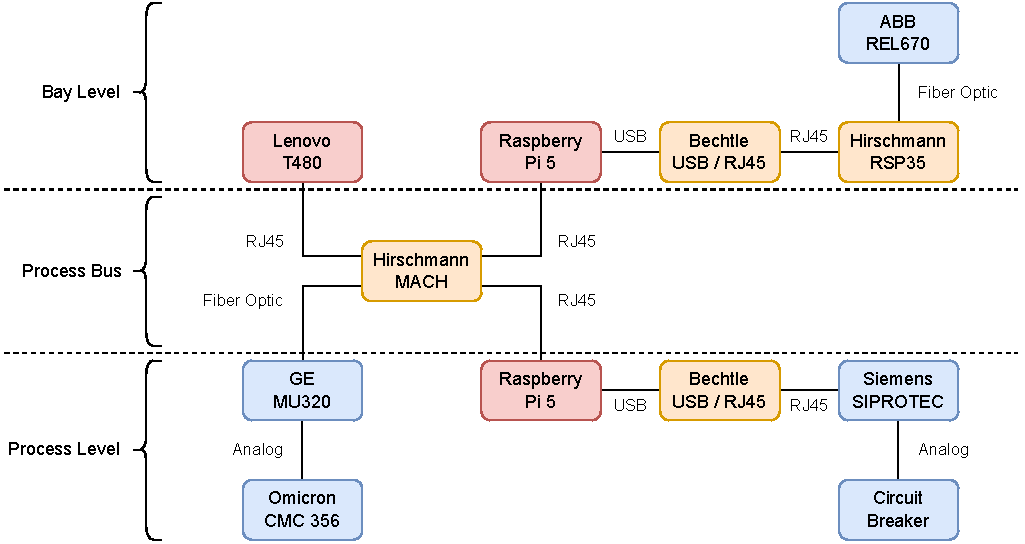
\includegraphics[width=1.0\linewidth]{figures/lab_evaluation_topology.drawio.pdf}
    \caption{Network topology of the laboratory-based experimental demonstration of applicability.}
    \label{fig:lab_topology}
\end{figure}

\subsection{Procedure \& Results}
\label{sec:evaluation:compatibility:procedure}
The procedure of the experiment comprised four key events.
The sequence of events and the corresponding messages exchanged between the devices are shown in \autoref{fig:lab_steps} and are discussed in the following:
\begin{description}
    \item[Step 1: Generate Overcurrent]~\\
    At the initial state of the experiment, the voltages and currents of all three phases generated by the Omicron CMC 356 were within certain boundaries to be detected as normal grid situation.
    Accordingly, the circuit breaker connected to the IED was closed and allowed power to flow through the grid.
    To start the experiment, we manually adjusted the generated three-phase electric power.
    The current was set to a higher level to simulate an overcurrent situation in the grid.
    This situation was communicated to the MU via a direct analog connection, i.e., the MU was measuring the voltages and currents of the three phases.

    \item[Step 2: Send Sampled Values]~\\
    The MU sampled the voltage and current values provided by the relay test device.
    The sampled values were sent to the IED using the SV protocol.
    As the MU was not protected by a PEP, we bypassed the SV frames at the IED's PEP.
    For this purpose, we programmed a static bypass rule into the IED's PEP that analyzed Ethernet frames to detect and forward SV frames sent by the MU.

    \item[Step 3: Send Trip Signal]~\\
    The IED received and processed the SV frames, and detected the overcurrent situation.
    To resolve the overcurrent situation, the IED sent a GOOSE frame to the I/O box to open the circuit breaker.
    As the IED was protected by a PEP, the outgoing GOOSE frame was captured by the PEP and processed as discussed in \autoref{sec:approach:sabaac:accesscontrol}.
    The authenticated and authorized payload exchange message, which contained the GOOSE frame, was then forwarded to the PEP of the I/O box.
    The PEP verified the incoming payload exchange message, extracted the encapsulated GOOSE frame, and forwarded the GOOSE frame to the I/O box.

    \item[Step 4: Trigger Circuit Breaker]~\\
    The I/O box received the original GOOSE frame, which was sent by the IED.
    As the GOOSE frame signalled to the I/O box to open the circuit breaker, the I/O box used an analog signal to open the circuit breaker.
    At the end of the experiment, we were able to visually verify that the circuit breaker had opened successfully.
\end{description}
\begin{figure}
    \centering
    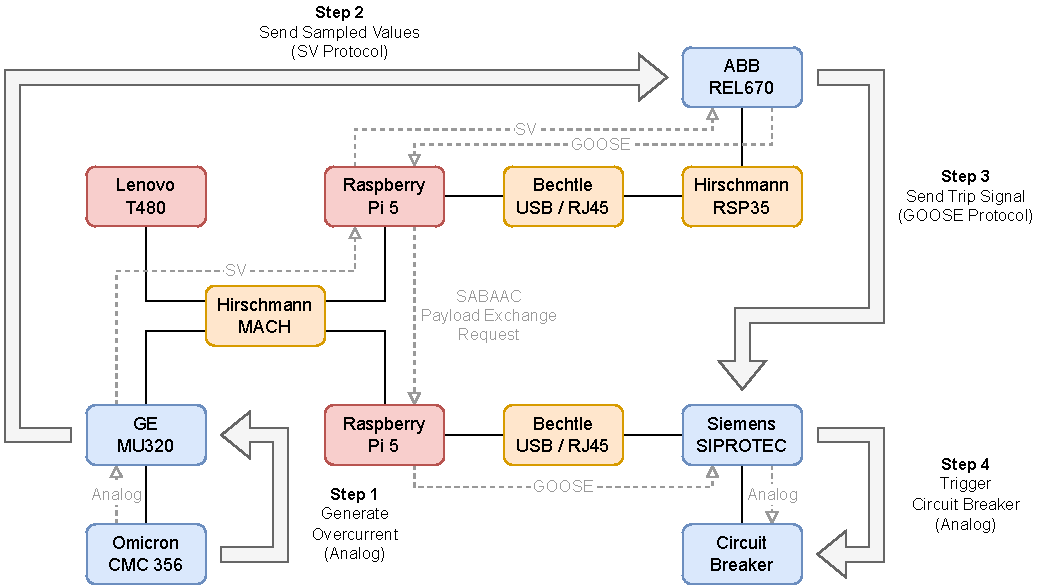
\includegraphics[width=1.0\linewidth]{figures/lab_evaluation_steps.drawio.pdf}
    \caption{Sequence of events of the laboratory-based experimental demonstration of applicability.}
    \label{fig:lab_steps}
\end{figure}

The simulated exception in the grid was successfully propagated through the SAS network during the experiment.
Consequently, the experiment demonstrated that the operation of the MU, IED, and I/O box was not disrupted by the employment of CASA and SABAAC.
Since we deployed the security-related components to inexpensive off-the-shelf hardware, we were able to demonstrate that our approach is a feasible solution for SAS environments not only security-wise and performance-wise but also cost-wise.
Due to the BITW concept of our approach, no adaptations had to be made to the SAS devices.
This indicates that our approach is a viable solution for the retrofitting of existing substations.
Furthermore, the usage of a static bypass rule in one of the PEPs suggests that incompatible or legacy devices could continue their operation in a retrofitted SAS.
Thus, the interoperability and interchangeability requirements of an IEC 61850 substation remain satisfied, while the communication security is increased by the enforcement of the CASC-SAS security policies.

\section{Discussion \& Comparison}
In this section we provide a summary of the findings of the evaluation, we contextualize our approach within the existing literature, and we describe the limitations and constraints inherent to the evaluation and our approach.
The conducted evaluation covered security, performance, and compatibility aspects of CASC-SAS, CASA, and SABAAC.
By performing a theoretical analysis of the security aspects of CASA and SABAAC, we demonstrated that our approaches are able to mitigate a set of adversarial attacks.
We proved that our signature scheme $S_{CASA}$ is existentially unforgeable under chosen-message attacks and that it resists collusion attacks under the DLP.
Furthermore, we provided definitions for message replay, forgery, modification, and time-delay attacks, and demonstrated how CASA and SABAAC interact to mitigate these attacks.
Our findings indicate that SAS devices benefit from being PEP-protected, as domain-typical DoS and false data injection attacks can be mitigated by the employment of our approach.
However, by employing CASA and SABAAC the attack surface of an SAS changes.
While IEDs, MUs, and other SAS devices benefit from being protected by using our BITW approach, the increased total number of devices in the SAS and their communication relations lead to an increased risk of DoS attacks.
In particular, the dependence on certain centralized components, such as the PDP, PAP, PSP, and CAPP, introduces new attack vectors for SAS adversaries.
Furthermore, as we conducted the security analysis theoretically, our findings might not be transferable to real SAS environments, and the behavior of CASA and SABAAC components under attack may be different from what we discussed theoretically.

In contrast to the security analysis, the performance and compatibility evaluations of our approach were conducted experimentally.
The results of both experimental evaluations suggest that CASA and SABAAC are able to secure time-critical communication in a SAS.
As we conducted the experiments using inexpensive off-the-shelf-hardware to deploy the CASC-SAS components, we demonstrated that our approach is lightweight and efficient with regard to its hardware requirements and corresponding deployment costs.
Nevertheless, the results of the performance evaluation indicate that computational performance is the primary challenge for the deployment of information security approaches in a SAS.
The findings demonstrate that lightweight yet inflexible symmetric cryptography approaches seem to be the only viable solution to secure low latency message exchanges.
However, the performance evaluation also revealed that the attribute-based authorization and access control workflows of SABAAC have only a limited impact on the overall message exchange latency.
Accordingly, the results emphasize the appropriateness of expressive and flexible yet computationally expensive access control approaches, such as ABAC, even in time and resource constrained environments.

Furthermore, the findings of the security, performance, and compatibility analysis indicate that authentication, authorization, and access control benefit from the consolidation of competencies.
Related approaches that we discussed in \autoref{ch:relatedwork}, focus on either secure communication or access control in substations.
While existing approaches for the security of SAS communication, including the BITW security filter by \citeauthor{Ishchenko2018} \cite{Ishchenko2018}, and the FPGA-based GOOSE and SV hardware encryption by \citeauthor{Rodriguez2021} \cite{Rodriguez2021}, are optimal solutions under certain circumstances, we emphasize the advantages of malleable security systems.
By integrating CASA and SABAAC into a cybersecurity and cryptography architecture for SAS, our approach enables adaption to future requirements, while it maintains a well-defined set of provided services.
In particular, our algorithm-agnostic CASA approach demonstrated the advantages of a malleable cryptography platform by supporting the employment of different algorithms for different use cases within a single SAS.

\chapter{Conclusion}
\label{ch:conclusion}
%In this last chapter, we conclude the thesis by presenting the potential future work of the proposed approach.
%The potential future work is discussed in \autoref{sec:conclusion:future_work}.
%Furthermore, in \autoref{sec:conclusion:summary}, we present a summary of the contributions and findings of the thesis.
This concluding chapter presents a summary and potential future directions of our approach.
The potential future directions are discussed in detail in \autoref{sec:conclusion:future_work}.
In \autoref{sec:conclusion:summary} we provide a summary of the contributions and findings of the thesis.

\section{Future Directions}
\label{sec:conclusion:future_work}
% AB-PKC - Pure Cryptography
Our findings indicate that the CASC-SAS approach, its cryptographic approach CASA, and its authorization and access control approach SABAAC serve to enhance the communication security of a SAS.
Further research could be conducted to determine, whether this enhancement of security is also achievable by employing a purely cryptographic approach.
To answer this question, we propose the design and realization of an AB-PKC approach that satisfies the requirements of the SAS domain.
In contrast to cryptography-dependent but scheme-agnostic ABAC, as we proposed it in CASC-SAS, the AB-PKC approach could allow the accomplishment of additional security objectives, including privacy and anonymity.

% Encryption \& Decryption
In addition to the changes in the approach paradigm, further research might investigate whether the CASA approach could be expanded to encompass encryption and decryption in conjunction with its signing and verification operations.
While confidentiality for power systems via encryption is explicitly non-recommended for time-critical communication in the IEC standards \cite{IEC62351P6}, further research might elucidate how confidentiality can be achieved even in such time-critical systems.

% Hardware Cryptography Accelerators
With regard to the cryptographic services provided by CASA, further studies could be carried out to evaluate the advantages and disadvantages of hardware-based cryptography acceleration.
It is anticipated that the required computation time will decrease, leading to an increase in message throughput through the utilization of hardware accelerators for cryptographic algorithms.
However, factors such as algorithm compatibility, costs per acceleration unit, and computation time consistency may result in a less beneficial influence on the system than currently expected.

% NTP/PTP/ARP Support \& Time Consistency
The evaluation demonstrated that CASC-SAS is capable of securing application protocols of a SAS, as well as multipurpose transport protocols.
However, network time protocols, such as the Network Time Protocol (NTP) and the Precision Time Protocol (PTP), were bypassed by the PEP entities, as the operation of these protocols is susceptible to temporal inconsistencies resulting from authentication and access control.
Further research could investigate how network time protocols could benefit from being processed by a PEP and what additional requirements and constraints have to be satisfied with regard to computation performance and time consistency.
Moreover, lower-layer network management protocols, such as the Address Resolution Protocol (ARP), were bypassed since these protocols provide services not only to SAS devices but also to auxiliary intermediate devices, including network switches and routers.
Future studies could evaluate the feasibility of CASC-SAS to process these network management protocols and mitigate attacks related to them.

% Redundancy Protocols
Furthermore, future studies could investigate the impact of redundancy protocols in time-critical networks on the operation of our approach.
To this end, CASC-SAS could be deployed and assessed in systems utilizing the Parallel Redundancy Protocol (PRP) or Media Redundancy Protocol (MRP).

% Implementation of CASC-SAS in Switch/SDN Controller
To simplify the architectural complexity of CASC-SAS, reduce the overall costs of deployment, and enable processing of the above-mentioned network protocols, we propose the integration of CASC-SAS into network switches as an alternative realization approach.
For this purpose, further research could investigate the potential benefits of realizing CASC-SAS through the use of Software-Defined Networking (SDN) solutions.
This SDN-based CASC-SAS could aggregate the tasks of multiple PEPs by deploying a virtual PEP for each port of a network switch.
Furthermore, distributed SDN controllers might provide the PAP, PSP, PDP, and CAPP services.

% AI for Policy Management
While the proposed PAP entities provide policy management services for human operators, future research could investigate how CASC-SAS might benefit from the utilization of artificial intelligence (AI).
The integration of AI-based intrusion detection could facilitate the creation and modification of security policies that are enforced within a SAS, thereby enabling our approach to mitigate a wider range of cyberattacks in a timelier manner.

% Deployment of CASC-SAS in Time-Critical Non-SAS Enviroments
In addition to the deployment in a SAS, further research is required to evaluate the applicability of CASC-SAS for other time-critical systems.
Therefore, we propose the evaluation of our approach in time-critical systems that have similar requirements as a SAS.
Systems that might potentially benefit from the enhanced communication security provided by our approach include industry 4.0, robotics, avionics, and medical systems.

\section{Summary}
\label{sec:conclusion:summary}
To address the increasing relevance of cybersecurity for smart grid systems and to overcome the limitations of existing standards like IEC 61850 and IEC 62351, we presented CASC-SAS, a novel cryptography and cybersecurity approach for the enhancement of SAS security.
The two attribute-based and server-aided approaches CASA and SABAAC represent the central parts of the four-layered dual-path CASC-SAS security architecture.

CASA provides algorithm-agnostic cryptographic protocols and services that serve as a foundation for the employment of other cryptography and cybersecurity mechanisms in a SAS.
The main objective of CASA is to enable and support secure authentication procedures that safeguard the integrity, authenticity, and non-repudiation of SAS communication.
As a central component of the CASA approach we presented the CAPP, an algorithm-agnostic administration and processing platform that provides key generation, key distribution, key revocation, and server-aided computation services via our APEX protocol to resource-constrained devices of a SAS.
Furthermore, in order to take the time-criticality of communication in a SAS into account, we discussed the importance and advantages of precomputation and server-aided computation for cryptographic procedures.
We demonstrated the viability of these computation techniques by presenting our server-aided AB-PKC signature scheme $S_{CASA}$.

SABAAC enables the administration and enforcement of ABAC policies for time-critical and time-variable environments.
We introduced the concept of time-dependency for attributes and ABAC policies, and discussed methods to manage, distribute, and enforce such expressive and flexible yet computationally expensive access control policies.
With regard to the management and evaluation of access control policies, we proposed a delegated attribute-based authorization protocol responsible for the policy creation, management, storage, and distribution.
With regard to the enforcement of policies, we introduced a delegated attribute-based access control protocol.
To facilitate the enforcement of policies in time-critical systems, we presented novel policy enforcement strategies, which combine server-side precomputation and client-side caching of access decisions.

We implemented CASA and SABAAC in software and deployed it to a hardware testbed.
The software is implemented component-wise using primarily the object-oriented high-level programming languages Java and Kotlin.
The software implementation of our approach is published open source on GitHub \cite{gitcasc} under the European Union Public Licence (EUPL) \cite{eupl}.
To assess the applicability of our approach for SAS environments, we conducted a theoretical and experimental evaluation.
%The experiments and evaluation results were published open source alongside the implementation.
The theorem-based theoretical security analysis has shown that CASC-SAS is capable of enhancing the communication security of a SAS by mitigating domain-typical adversarial attacks performed by a Dolev-Yao-like adversary.
We demonstrated that our approach mitigates, among others, message forgery, modification, replay, and time-delay attacks.
While SAS-typical cyberattacks can be mitigated by employing our approach, we also discussed the change of the attack surface, leading to an increased risk of DoS as a result of the additional components and protocols deployed in a SAS.
Based on the testbed implementation, the performance analysis demonstrated the ability of the approach to secure time-critical message exchanges.
Furthermore, the performance analysis identified the advantages and disadvantages of different authentication schemes with regard to satisfied time constraints.
In accordance with the related literature, we identified the strict time constraints of low latency communication in a SAS as a key challenge for information security.
The compatibility analysis demonstrated that our approach is a feasible solution for SAS environments not only security-wise and performance-wise but also cost-wise and due to its highly-compatible BITW concept, which allows retrofitting of existing systems.
As we conducted a laboratory-based demonstration of applicability, our evaluation demonstrated the ability of our approach to secure time-critical message exchanges of the GOOSE and SV protocol between an IED made by ABB, a MU made by General Electric, and an I/O box made by Siemens.
Accordingly, the results of the evaluation of our approach indicate that CASA and SABAAC are viable solutions to enhance the communication security in a newly constructed or retrofitted substation.


%% ---------------------------
%% |   Glossary / Acronyms   |
%% ---------------------------
% Glossary and acronyms are printed as chapter*: Used entries and non-empty chapters only!
\printglossary
\printacronyms

%% --------------------
%% |   Bibliography   |
%% --------------------

%% Add entry to the table of contents for the bibliography
\printbibliography[heading=bibintoc]

%% ----------------
%% |   Appendix   |
%% ----------------
% \appendix
% \chapter{Appendix}
\label{chap:appendix}
\section{Review Questions \& Responses}
\begin{enumerate}[label=Q\arabic*.]
    % Ghada's Questions
    \item \textit{Unclear context of OT-related cybersecurity incidents (p. 2)} --- The context of the cybersecurity incidents was clarified by rephrasing the sentence and moving the citation to a more appropriate position.
    \item \textit{Textual citation of 3 or more authors should be shortened to et al. (p. 2 ff.)} --- The maximum number of author names in textual citations was limited to two, e.g., (Elbez, Keller, and Hagenmeyer [16]) becomes (Elbez et al. [16]).
    \item \textit{Typo in the word therefore (p. 2)} --- A missing letter was added to the word therefore.
    \item \textit{Research questions should relate to previously described challenges, and RQ1 and RQ2 should differ more from each other (p. 2)} --- All three research questions were partially reconstructed to relate to the security objectives. Moreover, the research questions were rephrased to clarify their goals.
    \item \textit{Interchanged words in contribution section (p. 3)} --- The corresponding sentence was rephrased.
    \item \textit{To which extent is the SABAAC approach flexible (p. 3)} --- Since its policies and not the approach is expressive and flexible, the sentence was rephrased. Moreover, the expressiveness, flexibility, and computationally expensiveness of the policies were further clarified.
    \item \textit{It would be good to relate the fundamentals to the field of application (p. 6)} --- Since the fundamentals were shortened from twenty to two pages, the relations between its topics and the OT/ICS/SAS-domain were lost. Moreover, the relevance of the more abstract topics including access control and cryptography for the OT-domain is not sufficiently described in the proposal. This will be added to the fundamentals chapter of the thesis, as the realization is currently an open question.
    \item \textit{A paragraph could be added to relate the related work chapter to the fundamentals (p. 7)} --- This relation is present in the long thesis proposal in the form of a division into sections, which are related to topics of the fundamentals.
    \item \textit{Please consider organizing the related work into sections (p. 7)} --- This organization is present in the long thesis proposal and will be transferred to the final master's thesis. Moreover, an extension for the cryptography-specific related work is planned.
    \item \textit{Please consider discussing some limitations of related works on ABAC and RBAC to justify the motivation of your work (p. 8)} --- The similarities and differences of the thesis and related work as well as the limitations of related work are present in the long thesis proposal.
    \item \textit{Cybersecurity and cryptography are names of CASC-SAS layers (p. 9)} --- The differences of the two layers are discussed in detail in the long thesis proposal. However, since the two words cybersecurity and cryptography are closely related, renaming or renumbering of the layers is currently under consideration.
    \item \textit{For ease of read, better present requirements as a list (p. 10)} --- In the long thesis proposal the requirements and their short descriptions are presented as a list.
    \item \textit{How does the integration of CASA effectively relate to figure 4.2 (p. 13)} --- This figure caption was shortened, and the CASA-specific part was removed for better understandability.
    \item \textit{Which adversarial attacks would be relevant as use cases (p. 16)} --- A subsection in the system model dedicated to relevant attacks and attack trees is planned for the final thesis. Moreover, relevant attacks were added to the short proposal's requirements section. Due to the limited space in the short proposal, no attack-specific section with enumerated attacks was added.
    \item \textit{Which considerations would be included in the economic evaluation (p. 16)} --- Besides the aspects mentioned in the proposal, metrics such as the cost of CASC-SAS equipment will be discussed in the economic evaluation. Moreover, the economic evaluation covers the compatibility-related requirements, including interoperability and interchangeability, which are core concepts of the IEC 61850.
    \item \textit{Which evaluation aspects are possible theoretically (p. 16)} --- The theoretical evaluation covers the security proofs of CASA, the economic evaluation, and the calculation of minimum transfer time requirements for the performance evaluation. The theoretical approaches used will be discussed in detail in the corresponding evaluation sections in the thesis.
    \item \textit{Are times in the work plan total times and are increments processed in parallel (p. 17)} --- To clarify the total durations of milestones and parallel execution of increments, a sentence was added to the work plan introduction.
    \item \textit{Shouldn't software design flaws be considered before software implementation flaws (p. 20)} --- The order of the risks was changed to clarify that the design should be flawless before the implementation.
    % Ramadan's Questions
    \item \textit{The figure captions are too long} --- All figure captions in the proposal were shortened.
    \item \textit{The fundamentals are lacking a cryptography section} --- A cryptography section covering symmetric and asymmetric cryptography was added to the fundamentals of the long proposal.
    \item \textit{The NIST recommendations for access control are not discussed in the fundamentals} --- A NIST recommendations section was added to the fundamentals of the long proposal.
    \item \textit{The security model of CASA makes very strong statements about EUF-CMA, which are not correct anymore} --- The strong statement was removed from the security model and the section was rephrased.
    \item \textit{The introduction chapter lacks an objective section} --- A section for the objective of the thesis was added to the introduction chapter. Moreover, the already existing research question section was integrated into the new section.
    \item \textit{The introduction chapter lacks a thesis structure section} --- A section for the proposed structure of the thesis was added to the introduction chapter of the long proposal. Moreover, a graphical representation of the structure is currently under consideration.
    \item \textit{The typical cybersecurity incidents mentioned in related work are not present in the objective of the approach} --- A paragraph for cybersecurity incidents was added to the objective section.
    % Meeting Questions
    \item \textit{Sender and receiver are interchanged in SABAAC figures} --- The errors in the SABAAC figures were fixed.
    \item \textit{SABAAC is misspelled in the time schedule} --- The error in the time schedule figure was fixed.
    \item \textit{A deprecated security requirement is present in the CASA description in the long proposal} --- The deprecated security requirement was removed.
    \item \textit{Prof. Dr. Veit Hagenmeyer is the first examiner of the thesis} --- The examiners on the title page of the short and long proposal were changed. However, the second examiner is currently unknown.
    \item \textit{Missing group logo at title page} --- The KASTEL logo was added to the title page as group logo. Note: This change was reverted for the template version of the proposal.
    \item \textit{Citations should be numbered in the order in which they appear} --- The ordering of the bibliography was changed.
    \item \textit{State-sponsored cybersecurity incidents included summary of incidents from 2013 to 2020 (p. 2)} --- The mentioning of non-discussed but referenced incidents from 2013 to 2020 was removed.
    \item \textit{Ordering of research questions is not consistent with main thesis focus ABAC (p. 2)} --- Changed order of RQ1 and RQ2.
    \item \textit{RQ2 and RQ3 contain concepts of contribution and shrink the solution space too much (p. 2)} --- Revised research questions by replacing concrete concepts such as certificateless and server-aided with more goal-oriented and unbiased terms such as lightweight and scalable.
    \item \textit{Introduction chapter lacks an enumeration of thesis contributions (p. 3)} --- The contribution section was rephrased and restructured. The contributions are now presented as an enumeration.
    \item \textit{The asymmetric cryptography section should be renamed to PKC and lacks a description of symmetric cryptography (p. 5)} --- The PKC section was renamed and a sentence to distinguish symmetric from asymmetric algorithms was added. The long version of the proposal contains an own section for symmetric cryptography.
    \item \textit{The economic evaluation is not possible due to missing data and the term economic/economy should be avoided (p. 16)} --- The third evaluation area was renamed to compatibility, to emphasize the new focus on interoperability and interchangeability as defined in IEC 61850, and the focus on economy in this area was reduced by rephrasing and restructuring.
    \item \textit{Overlapping increments of time schedule do not seem feasible (p. 19)} --- The realization phase was extended, and the evaluation phase was shortened by two weeks. Moreover, the increment durations and starting dates were revised to reduce overlapping phases.
    \item \textit{The title page should present meta information differently} --- The title page text and the thesis TeX class were changed.
    \item \textit{Project plan chapter should be renamed to thesis plan} --- The chapter was renamed. Moreover, the term project was replaced with the term thesis at appropriate locations in the text.
\end{enumerate}


\end{document}
